\documentclass[onecolumn, compsoc,10pt]{IEEEtran}
\let\labelindent\relax
\usepackage{enumitem}
\usepackage{etex}
\usepackage{amssymb,amsfonts,amsmath,amsthm}
\usepackage{graphicx}
\usepackage{booktabs}
\usepackage[usenames,x11names, dvipsnames, svgnames]{xcolor}
\usepackage{amsmath,amssymb}
\usepackage{dsfont}
\usepackage{amsfonts}
\usepackage{mathrsfs}
\usepackage{texshade}
\usepackage{hyperref}
\hypersetup{
  colorlinks=true,
  linkcolor=black,
  citecolor=blue,
  filecolor=black,
  urlcolor=DodgerBlue4,
  breaklinks=false,
  % linkbordercolor=red,% hyperlink borders will be red
  % pdfborderstyle={/S/U/W 1}% border style will be underline of width 1pt
}
\usepackage{array}
\usepackage{xr}
\usepackage{verbatim}
\usepackage{multirow}
\usepackage{longtable}
\usepackage{tikz-network}
\usepackage[T1,euler-digits]{eulervm}
\usepackage{times}
% \usepackage{pxfonts}
\usepackage{tikz}
\usepackage{pgfplots}
\usetikzlibrary{shapes,calc,shadows,fadings,arrows,decorations.pathreplacing,automata,positioning}
\usetikzlibrary{external}
\usetikzlibrary{decorations.text}
\usepgfplotslibrary{colorbrewer} 
\usepgfplotslibrary{statistics}

\tikzexternalize[prefix=./Figures/External/]% activate externalization!
\tikzexternaldisable
% \addtolength{\voffset}{.1in}  
\usepackage{geometry}
\geometry{letterpaper, left=.6in,right=.6in,top=.5in,bottom=0.7in}

%\addtolength{\textwidth}{-.1in}    
%\addtolength{\hoffset}{.05in}    
%\addtolength{\textheight}{.1in}    
%\addtolength{\footskip}{0in}    
\usepackage{rotating}
\definecolor{nodecol}{RGB}{240,240,220}
\definecolor{nodeedge}{RGB}{240,240,225}
\definecolor{edgecol}{RGB}{130,130,130}
\tikzset{%
  fshadow/.style={      preaction={
      fill=black,opacity=.3,
      path fading=circle with fuzzy edge 20 percent,
      transform canvas={xshift=1mm,yshift=-1mm}
    }} 
}
\usetikzlibrary{pgfplots.dateplot}
\usetikzlibrary{patterns}
\usetikzlibrary{decorations.markings}
\usepackage{fancyhdr}
\usepackage{mathtools}
\usepackage{datetime}
\usepackage{comment}
%% ## Equation Space Control---------------------------
\def\EQSP{3pt}
\newcommand{\mltlne}[2][\EQSP]{\begingroup\setlength\abovedisplayskip{#1}\setlength\belowdisplayskip{#1}\begin{equation}\begin{multlined} #2 \end{multlined}\end{equation}\endgroup\noindent}
\newcommand{\cgather}[2][\EQSP]{\begingroup\setlength\abovedisplayskip{#1}\setlength\belowdisplayskip{#1}\begin{gather} #2 \end{gather}\endgroup\noindent}
\newcommand{\cgathers}[2][\EQSP]{\begingroup\setlength\abovedisplayskip{#1}\setlength\belowdisplayskip{#1}\begin{gather*} #2 \end{gather*}\endgroup\noindent}
\newcommand{\calign}[2][\EQSP]{\begingroup\setlength\abovedisplayskip{#1}\setlength\belowdisplayskip{#1}\begin{align} #2 \end{align}\endgroup\noindent}
\newcommand{\caligns}[2][\EQSP]{\begingroup\setlength\abovedisplayskip{#1}\setlength\belowdisplayskip{#1}\begin{align*} #2 \end{align*}\endgroup\noindent}
\newcommand{\mnp}[2]{\begin{minipage}{#1}#2\end{minipage}} 
%% COLOR DEFS------------------------------------------
\newtheorem{thm}{Theorem}
\newtheorem{cor}{Corollary}
\newtheorem{lem}{Lemma}
\newtheorem{prop}{Proposition}
\newtheorem{defn}{Definition}
\newtheorem{exmpl}{Example}
\newtheorem{rem}{Remark}
\newtheorem{notn}{Notation}
%% ------------PROOF INCLUSION -----------------
\def\NOPROOF{Proof omitted.}
\newif\ifproof
\prooffalse % or \draftfalse
\newcommand{\Proof}[1]{
  \ifproof
  \begin{IEEEproof}
    #1\end{IEEEproof}
  \else
  \NOPROOF
  \fi
}
%% ------------ -----------------
\newcommand{\DETAILS}[1]{#1}
%% ------------ -----------------
% color commands------------------------
\newcommand{\etal}{\textit{et} \mspace{3mu} \textit{al.}}
% \renewcommand{\algorithmiccomment}[1]{$/** $ #1 $ **/$}
\newcommand{\vect}[1]{\textbf{\textit{#1}}}
\newcommand{\figfont}{\fontsize{8}{8}\selectfont\strut}
\newcommand{\hlt}{ \bf \sffamily \itshape\color[rgb]{.1,.2,.45}}
\newcommand{\pitilde}{\widetilde{\pi}}
\newcommand{\Pitilde}{\widetilde{\Pi}}
\newcommand{\bvec}{\vartheta}
\newcommand{\algo}{\textrm{\bf\texttt{GenESeSS}}\xspace}
\newcommand{\xalgo}{\textrm{\bf\texttt{xGenESeSS}}\xspace}
\newcommand{\FNTST}{\bf }
\newcommand{\FNTED}{\color{darkgray} \scriptsize $\phantom{.}$}
\renewcommand{\baselinestretch}{.9}
\newcommand{\sync}{\otimes}
\newcommand{\psync}{\hspace{3pt}\overrightarrow{\hspace{-3pt}\sync}}
% \newcommand{\psync}{\raisebox{-4pt}{\begin{tikzpicture}\node[anchor=south] (A) {$\sync$};
%   \draw [->,>=stealth] ([yshift=-2pt, xshift=2pt]A.north west) -- ([yshift=-2pt]A.north east); %\end{tikzpicture}}}
\newcommand{\base}[1]{\llbracket #1 \rrbracket}
\newcommand{\nst}{\textrm{\sffamily\textsc{Numstates}}}
\newcommand{\HA}{\boldsymbol{\mathds{H}}}
\newcommand{\eqp}{ \vartheta }
\newcommand{\entropy}[1]{\boldsymbol{h}\left ( #1 \right )}
\newcommand{\norm}[1]{\left\lVert #1 \right\rVert}%
\newcommand{\abs}[1]{\left\lvert #1 \right\rvert}%
\newcommand{\absB}[1]{\big\lvert #1 \big\rvert}%
% #############################################################
% #############################################################
% PREAMBLE ####################################################
% #############################################################
% #############################################################
% \usepackage{pnastwoF}      
\DeclareMathOperator*{\argmax}{argmax}
\DeclareMathOperator*{\argmin}{arg\,min}
\DeclareMathOperator*{\expect}{\mathbf{E}}
\DeclareMathOperator*{\var}{\mathbf{Var}}

\newcommand{\ND}{ \mathcal{N}  }
\usepackage[linesnumbered,ruled,vlined,noend]{algorithm2e}
\newcommand{\captionN}[1]{\caption{\color{darkgray} \sffamily \fontsize{9}{10}\selectfont #1  }}
\newcommand{\btl}{\ \textbf{\small\sffamily bits/letter}}
%\usepackage{txfonts}
%%% \usepackage{ccfonts}
%%% save defaults
%\renewcommand{\rmdefault}{phv} % Arial
%\renewcommand{\sfdefault}{phv} % Arial
%\edef\keptrmdefault{\rmdefault}
%\edef\keptsfdefault{\sfdefault}
%\edef\keptttdefault{\ttdefault}

% \usepackage{kerkis}
%\usepackage[OT1]{fontenc}
%\usepackage{concmath}
% \usepackage[T1]{eulervm} 
% \usepackage[OT1]{fontenc}
%%% restore defaults
%\edef\rmdefault{\keptrmdefault}
%\edef\sfdefault{\keptsfdefault}
%\edef\ttdefault{\keptttdefault}
\tikzexternalenable
% ##########################################################
\tikzfading[name=fade out,
inner color=transparent!0,
outer color=transparent!100]
% ###################################
\newcommand{\xtitaut}[2]{
  \noindent\mnp{\textwidth}{
    \mnp{\textwidth}{\raggedright\Huge \bf \sffamily #1}

    \vskip 1em

    {\bf \sffamily #2}
  }
  \vskip 2em
}
% ###################################
% ###################################
\tikzset{wiggle/.style={decorate, decoration={random steps, amplitude=10pt}}}
\usetikzlibrary{decorations.pathmorphing}
\pgfdeclaredecoration{Snake}{initial}
{
  \state{initial}[switch if less than=+.625\pgfdecorationsegmentlength to final,
  width=+.3125\pgfdecorationsegmentlength,
  next state=down]{
    \pgfpathmoveto{\pgfqpoint{0pt}{\pgfdecorationsegmentamplitude}}
  }
  \state{down}[switch if less than=+.8125\pgfdecorationsegmentlength to end down,
  width=+.5\pgfdecorationsegmentlength,
  next state=up]{
    \pgfpathcosine{\pgfqpoint{.25\pgfdecorationsegmentlength}{-1\pgfdecorationsegmentamplitude}}
    \pgfpathsine{\pgfqpoint{.25\pgfdecorationsegmentlength}{-1\pgfdecorationsegmentamplitude}}
  }
  \state{up}[switch if less than=+.8125\pgfdecorationsegmentlength to end up,
  width=+.5\pgfdecorationsegmentlength,
  next state=down]{
    \pgfpathcosine{\pgfqpoint{.25\pgfdecorationsegmentlength}{\pgfdecorationsegmentamplitude}}
    \pgfpathsine{\pgfqpoint{.25\pgfdecorationsegmentlength}{\pgfdecorationsegmentamplitude}}
  }
  \state{end down}[width=+.3125\pgfdecorationsegmentlength,
  next state=final]{
    \pgfpathcosine{\pgfqpoint{.15625\pgfdecorationsegmentlength}{-.5\pgfdecorationsegmentamplitude}}
    \pgfpathsine{\pgfqpoint{.15625\pgfdecorationsegmentlength}{-.5\pgfdecorationsegmentamplitude}}
  }
  \state{end up}[width=+.3125\pgfdecorationsegmentlength,
  next state=final]{
    \pgfpathcosine{\pgfqpoint{.15625\pgfdecorationsegmentlength}{.5\pgfdecorationsegmentamplitude}}
    \pgfpathsine{\pgfqpoint{.15625\pgfdecorationsegmentlength}{.5\pgfdecorationsegmentamplitude}}
  }
  \state{final}{\pgfpathlineto{\pgfpointdecoratedpathlast}}
}
% ###################################
% ###################################
\newcolumntype{L}[1]{>{\rule{0pt}{2ex}\raggedright\let\newline\\\arraybackslash\hspace{0pt}}m{#1}}
\newcolumntype{C}[1]{>{\rule{0pt}{2ex}\centering\let\newline\\\arraybackslash\hspace{0pt}}m{#1}}
\newcolumntype{R}[1]{>{\rule{0pt}{2ex}\raggedleft\let\newline\\\arraybackslash\hspace{0pt}}m{#1}}



% ################################################
% ################################################
% ################################################
% ################################################
\def\DISCLOSURE#1{\def\disclosure{#1}}
\DISCLOSURE{\raisebox{15pt}{$\phantom{XxxX}$This sheet contains proprietary information 
    not to be released to third parties except for the explicit purpose of evaluation.}
}
% ####################################
\newcommand{\set}[1]{\left\{ #1 \right\}}
\newcommand{\paren}[1]{\left( #1 \right)}
\newcommand{\bracket}[1]{\left[ #1 \right]}
% \newcommand{\norm}[1]{\left\Vert #1 \right\Vert}
\newcommand{\nrm}[1]{\left\llbracket{#1}\right\rrbracket}
\newcommand{\parenBar}[2]{\paren{#1\,{\left\Vert\,#2\right.}}}
\newcommand{\parenBarl}[2]{\paren{\left.#1\,\right\Vert\,#2}}
\newcommand{\ie}{$i.e.$\xspace}
\newcommand{\addcitation}{\textcolor{black!50!red}{\textbf{ADD CITATION}}}
\newcommand{\subtochange}[1]{{\color{black!50!green}{#1}}}
\newcommand{\tobecompleted}{{\color{black!50!red}TO BE COMPLETED.}}


\newcommand{\pIn}{\mathscr{P}_{\textrm{in}}}
\newcommand{\pOut}{\mathscr{P}_{\textrm{out}}}
\newcommand{\aIn}[1][\Sigma]{#1_{\textrm{in}}}
\newcommand{\aOut}[1][\Sigma]{#1_{\textrm{out}}}
\newcommand{\xin}[1]{#1_{\textrm{in}}}
\newcommand{\xout}[1]{#1_{\textrm{out}}}

\newcommand{\R}{\mathbb{R}} % Set of real numbers
\newcommand{\F}[1][]{\mathcal{F}_{#1}}
\newcommand{\SR}{\mathcal{S}} % Semiring of sets
\newcommand{\RR}{\mathcal{R}} % Ring of sets
\newcommand{\N}{\mathbb{N}} % Set of natural numbers (0 included)


\newcommand{\Pp}[1][n]{\mathscr{P}^+_{#1}}
\renewcommand{\entropy}[1]{\boldsymbol{h}\left ( #1 \right )}



\makeatletter
\pgfdeclarepatternformonly[\hatchdistance,\hatchthickness]{flexible hatch}
{\pgfqpoint{0pt}{0pt}}
{\pgfqpoint{\hatchdistance}{\hatchdistance}}
{\pgfpoint{\hatchdistance-1pt}{\hatchdistance-1pt}}%
{
  \pgfsetcolor{\tikz@pattern@color}
  \pgfsetlinewidth{\hatchthickness}
  \pgfpathmoveto{\pgfqpoint{0pt}{0pt}}
  \pgfpathlineto{\pgfqpoint{\hatchdistance}{\hatchdistance}}
  \pgfusepath{stroke}
}
\makeatother

\pgfdeclarepatternformonly{north east lines wide}%
{\pgfqpoint{-1pt}{-1pt}}%
{\pgfqpoint{10pt}{10pt}}%
{\pgfqpoint{9pt}{9pt}}%
{
  \pgfsetlinewidth{0.7pt}
  \pgfpathmoveto{\pgfqpoint{0pt}{0pt}}
  \pgfpathlineto{\pgfqpoint{9.1pt}{9.1pt}}
  \pgfusepath{stroke}
}

\pgfdeclarepatternformonly{north west lines wide}%
{\pgfqpoint{-1pt}{-1pt}}%
{\pgfqpoint{10pt}{10pt}}%
{\pgfqpoint{9pt}{9pt}}%
{
  \pgfsetlinewidth{0.7pt}
  \pgfpathmoveto{\pgfqpoint{0pt}{9pt}}
  \pgfpathlineto{\pgfqpoint{9.1pt}{-0.1pt}}
  \pgfusepath{stroke}
}
\makeatletter

\pgfdeclarepatternformonly[\hatchdistance,\hatchthickness]{flexible hatchB}
{\pgfqpoint{0pt}{\hatchdistance}}
{\pgfqpoint{\hatchdistance}{0pt}}
{\pgfpoint{1pt}{\hatchdistance-1pt}}%
{
  \pgfsetcolor{\tikz@pattern@color}
  \pgfsetlinewidth{\hatchthickness}
  \pgfpathmoveto{\pgfqpoint{0pt}{\hatchdistance}}
  \pgfpathlineto{\pgfqpoint{\hatchdistance}{0pt}}
  \pgfusepath{stroke}
}    \makeatother


\def\TPR{\textrm{TPR}\xspace}
\def\TNR{\textrm{TNR}\xspace}
\def\FPR{\textrm{FPR}\xspace}
\def\PPV{\textrm{PPV}\xspace}

\usetikzlibrary{arrows.meta}
\usetikzlibrary{decorations.pathreplacing,shapes.misc}
\usepgfplotslibrary{fillbetween}
%usepackage{tikz-network}
\usetikzlibrary{shapes.geometric}
\usetikzlibrary{math}
\usepgfplotslibrary{colorbrewer} 

\usepackage{textcomp}
\usepackage{colortbl}
\usepackage{array}
\usepackage{courier} 
\usepackage{wrapfig}
\usepackage{pifont}
\usetikzlibrary{chains,backgrounds}
\usetikzlibrary{intersections}
\usetikzlibrary{pgfplots.groupplots}
\usepgfplotslibrary{fillbetween} 
\usetikzlibrary{arrows.meta}
\usepackage{pgfplotstable}
\usepackage[super,compress,sort,comma]{natbib}
%\usepackage{natbib}
\usepackage{setspace}
\usetikzlibrary{math}
\usetikzlibrary{matrix}
\usepackage{xstring}
\usepackage{xspace}
\usepackage{flushend}
\makeatletter
\renewcommand\section{\@startsection {section}{1}{\z@}%
  {-2ex \@plus -1ex \@minus -.2ex}%
  {1ex \@plus.1ex}%
  {\Large\bfseries\scshape}}
\renewcommand\subsection{\@startsection {subsection}{1}{\z@}%
  {-2ex \@plus -.25ex \@minus -.2ex}%
  {0.1ex \@plus.0ex}%
  {\fontsize{11}{10}\selectfont\bfseries\sffamily\color{black}}}
\renewcommand\subsubsection{\@startsection {subsubsection}{1}{\z@}%
  {0ex \@plus -.5ex \@minus -.2ex}%
  {0.0ex \@plus.5ex}%
  {\bfseries\itshape\sffamily\color{darkgray}}}
\renewcommand\paragraph{\@startsection {paragraph}{1}{\z@}%
  {-.2ex \@plus -.5ex \@minus -.2ex}%
  {0.0ex \@plus.5ex}%
  {\fontsize{9}{9}\selectfont\itshape\sffamily\color{darkgray}}}
       
%\renewcommand{\thesubsection}{\thesection.\arabic{subsection}}
\renewcommand{\thesubsectiondis}{\arabic{subsection}.}
\renewcommand{\thesectiondis}{\arabic{section}.}
\renewcommand{\thesection}{\arabic{section}}

\renewcommand{\thetable}{\arabic{table}}

\makeatother
\makeatletter
\pgfdeclareradialshading[tikz@ball]{ball}{\pgfqpoint{-10bp}{10bp}}{%
  color(0bp)=(tikz@ball!30!white);
  color(9bp)=(tikz@ball!75!white);
  color(18bp)=(tikz@ball!90!black);
  color(25bp)=(tikz@ball!70!black);
  color(50bp)=(black)}
\makeatother
%\newcommand{\tball}[1][CadetBlue4]{${\color{#1}\Large\boldsymbol{\blacksquare}}$}
\renewcommand{\baselinestretch}{1}
%\renewcommand{\captionN}[1]{\caption{\color{CadetBlue4!50!black} \sffamily \fontsize{9}{10}\selectfont #1  }}
\tikzexternaldisable 
\parskip=6pt
\parindent=0pt
%\newcommand{\Mark}[1]{\textsuperscript{#1}}
\pagestyle{fancy}

\newcounter{Dcounter}
\setcounter{Dcounter}{1}
\newcommand{\DQS}[1]{\marginpar{\tikzexternaldisable \tikz{\node[rounded corners=5pt,draw=none,thick,fill=black!10,font=\sffamily\fontsize{7}{8}\selectfont] {\mnp{.45in} {\color{Red3}\raggedright  \#\theDcounter.~#1}}; }}\stepcounter{Dcounter}\xspace}

\newcommand{\qn}[1][i]{\Phi_{#1}}
\newcommand{\D}[1][i]{\mathscr{D}\left ( {\Sigma_#1} \right ) }
\newcommand{\Dx}{\mathscr{D}}
\def\J{\mathds{J}}
\def\M{\omega}
\def\N{\mathds{N}}
\newcommand{\cp}[1][P]{\langle #1 \rangle}
\newcommand{\mem}[1]{\M_{#1}}


\makeatletter
\newcommand\transformxdimension[1]{
    \pgfmathparse{((#1/\pgfplots@x@veclength)+\pgfplots@data@scale@trafo@SHIFT@x)/10^\pgfplots@data@scale@trafo@EXPONENT@x}
}
\newcommand\transformydimension[1]{
    \pgfmathparse{((#1/\pgfplots@y@veclength)+\pgfplots@data@scale@trafo@SHIFT@y)/10^\pgfplots@data@scale@trafo@EXPONENT@y}
}
\makeatother

\parskip=6pt
\parindent=0pt


\pgfplotsset{
    discard if/.style 2 args={
        x filter/.code={
            \edef\tempa{\thisrow{#1}}
            \edef\tempb{#2}
            \ifx\tempa\tempb
                \def\pgfmathresult{inf}
            \fi
        }
    },
    discard if not/.style 2 args={
        x filter/.code={
            \edef\tempa{\thisrow{#1}}
            \edef\tempb{#2}
            \ifx\tempa\tempb
            \else
                \def\pgfmathresult{inf}
            \fi
        }
    }
  }

  %\newcommand{\HLT}[2][Red1]{{\color{#1}#2}}

 % \def\commatonone{\expandafter\zappointzerozero
%    \romannumeral`\^^@}
%\def\zappointzerozero#1.00{\zapcomma#1,!}
%\def\zapcomma#1,#2{#1\ifx!#2\else#2\expandafter\zapcomma\fi}
\def\commatononei#1,{#1}
\def\commatononej#1,#2,{#1#2}
\def\commatonone#1{\expandafter\commatononei#1}
\def\commatononeT#1{\expandafter\commatononej#1}
\newcommand{\Sum} [2] {#1 + #2 = \the\numexpr #1 + #2 \relax \\}


\usepackage{sistyle}
\SIthousandsep{,}

\makeatletter
\newcommand{\limitpages}[1]{
  \gdef\maxpages{#1}%
  \ifx\latex@outputpage\@undefined\relax%
  \global\let\latex@outputpage\@outputpage%
  \fi%
  \gdef\@outputpage{%
    \ifnum\value{page}>\maxpages\relax%
    % Do not output the page
    \else%
    \latex@outputpage%
    \fi%
  }%
}
\makeatother
\newcommand{\note}[1]{{ \itshape \footnotesize \color{Red1}$\medbullet$~ #1}}









\renewcommand{\thesectiondis}{\arabic{section}.}
\renewcommand{\thesubsectiondis}{\Alph{subsection}.}

\makeatletter
\renewcommand\section{\@startsection {section}{1}{\z@}%
  {-1pt \@plus -30ex \@minus 20ex}%
  {.1pt}%
  {\large\bfseries\scshape}}
\renewcommand\subsection{\@startsection {subsection}{2}{\z@}%
  {0ex \@plus -1.75ex \@minus -1.2ex}%
  {0ex \@plus.0ex}%
  {\fontsize{11}{11}\selectfont\bfseries\sffamily\color{black}}}
\renewcommand\subsubsection{\@startsection {section}{1}{\z@}%
  {-.1ex \@plus -.5ex \@minus -.2ex}%
  {0.0ex \@plus.5ex}%
  {\bfseries\sffamily\color{Red4}}}
\renewcommand\paragraph{\@startsection {section}{1}{\z@}%
  {-.1ex \@plus -.5ex \@minus -.2ex}%
  {0.0ex \@plus.5ex}%
  {\fontsize{11}{10}\selectfont\bfseries\itshape\sffamily\color{black}}}
\makeatother


\makeatletter
\pgfdeclareradialshading[tikz@ball]{ball}{\pgfqpoint{-10bp}{10bp}}{%
  color(0bp)=(tikz@ball!30!white);
  color(9bp)=(tikz@ball!75!white);
  color(18bp)=(tikz@ball!90!black);
  color(25bp)=(tikz@ball!70!black);
  color(50bp)=(black)}
\makeatother
\newcommand{\tball}{${\color{CadetBlue3}\Large\boldsymbol{\blacksquare}}$}
\renewcommand{\baselinestretch}{.87}
\newcommand{\VSP}{\vspace{-2pt}}
\renewcommand{\captionN}[1]{\caption{\color{black} \sffamily \fontsize{9}{10}\selectfont #1  }}




\newcommand*{\doi}[1]{\href{http://dx.doi.org/#1}{doi: #1}}
\renewcommand{\IEEEbibitemsep}{20pt plus 2pt}
\makeatletter
\IEEEtriggercmd{\reset@font\normalfont\fontsize{11}{14}\selectfont}
\makeatother
\IEEEtriggeratref{1}
\newlength{\bibitemsep}\setlength{\bibitemsep}{.2\baselineskip plus .05\baselineskip minus .05\baselineskip}
\newlength{\bibparskip}\setlength{\bibparskip}{0pt}
\let\oldthebibliography\thebibliography
\renewcommand\thebibliography[1]{%
  \oldthebibliography{#1}%
  \setlength{\parskip}{\bibitemsep}%
  \setlength{\itemsep}{\bibparskip}%
}
\setlength{\bibitemsep}{.3\baselineskip plus .05\baselineskip minus .05\baselineskip} 
\def\V{\mathds{V}}
\def\Appendix{Appendix}
%###################################

\newif\iftikzX
\tikzXtrue
\tikzXfalse
%--------------
\def\jobnameX{zero}
%--------------
\newif\ifFIGS
\FIGSfalse 
\FIGStrue
%--------------
\newif\ifdraftQ
\draftQtrue
%\draftQfalse
%--------------
%###################################
\def\TITLE{\LARGE \enet: Fast Scalable Pandemic Risk Estimation of  \infl Strains Collected In Non-human Hosts}
%\def\TITLE{\LARGE A Biologically Meaningful Sequence Metric\\For Analyzing Evolutionary Changes\\In Novel Pathogens}
%\def\TITLE{Learning  Mutational Patterns At Scale For\\Analysis Of Sequence Divergence\\In Novel Pathogens}
%\def\TITLE{Learning Mutational Patterns at Scale to Analyze Sequence Divergence in Novel Pathogens}

\def\authore{Kevin Wu}
\def\authora{ Jin Li}
\def\authorb{Timmy Li}
\def\authorc{Aaron Esser-Kahn}
\def\authord{Ishanu Chattopadhyay}

\def\addressa{Department of Medicine, University of Chicago, IL, USA}
\def\addressb{Committee on Genetics, Genomics \& Systems BioloScalegy, University of Chicago, IL, USA}
\def\addressc{Committee on Quantitative Methods in Social, Behavioral, and Health Sciences, University of Chicago, IL, USA}
\def\addressd{Pritzker School of Molecular Engineering, University of Chicago, Chicago, IL, USA}
\def\addresse{Committee on Immunology, University of Chicago, Chicago, IL, USA}
\newif\ifdraftQ
\draftQtrue
\draftQfalse


%###################################

\title{\TITLE}
\author{\sffamily  \fontsize{10}{12}\selectfont   \authore$^{1}$,\authora$^{1}$, \authorb$^{1}$,  \authorc$^{2,3}$, and \authord$^{1,4,5\bigstar}$\\                                                                
\vspace{10pt}                                                                   

\sffamily  \fontsize{10}{12}\selectfont                                         
$^{1}$\addressa\\   
$^{2}$\addressd\\
$^{3}$\addresse\\
$^{4}$\addressb\\
$^{5}$\addressc                                                                 
\vskip 1em                                                                      
$^\bigstar$To whom correspondence should be addressed: e-mail: \texttt{ishanu@uchicago.edu}.}


\def\hcov{SARS-CoV-2\xspace}
\def\RATG13{RaTG13\xspace}
\def\Appendix{Appendix}
\def\qnet{Qnet\xspace}
\def\enet{Emergenet\xspace}
\def\erisk{risk\xspace}
\def\qdist{E-distance\xspace}
\def\cov{COVID-19\xspace}
\def\infl{Influenza A\xspace}
%\def\infl{IAV\xspace}


\def\E{\mathcal{E}}
\def\dst{x_\star^{t+\delta}}
\def\dsta{x^{t+\delta}}

\usepackage{flushend}
\externaldocument[SI-]{SI}
% \externaldocument[EXT-]{exfig}
\newif\iftikzX
\tikzXtrue
\tikzXfalse
\def\Extended{}
\newif\ifFIGS
\FIGSfalse  
\FIGStrue
 
% \authorcontributions{%Please provide details of author contributions here.
% JL and TL implemented the algorithm, AE and IC interpreted results and worked on mathematical modeling and IC wrote the paper
% }

\tikzexternalenable   
%\pgfplotsset{compat=1.18}
\begin{document}  
 
\maketitle
 
  {\bf \sffamily \fontsize{10}{12}\selectfont \noindent   
    {\normalfont \itshape Abstract:} Influenza viruses can produce  small sequence alterations~\cite{dos2016influenza}  that sufficiently perturb surface protein structures to evade host immunity. Failing to closely predict the dominant strain in an upcoming season  dramatically reduces  the  effectiveness of the flu shot~\cite{tricco2013comparing}, yet such prediction still remains imperfect. Furthermore, novel strains emerging into humans from animal reservoirs, has  historically   posed the possibly graver threat of a global  pandemic~\cite{shao2017evolution,mills2004transmissibility,reid2003origin,landolt2007up}, and our current ability to  scalably  evaluate the pandemic potential of   individual strains  is severely limited. In this study, we introduce a computational approach to  parse out emergent evolutionary constraints using only genomic sequence data. A representation of these  inferred dependencies along with the associated computational framework is referred to as the \enet.   Analyzing    Hemaglutinnin (HA) and Neuraminidase (NA) amino acid sequences from nearly 100,000 unique \infl  strains from public  databases, our proposed computational tools  estimate the likelihood of a specific future  mutation, ultimately  yielding the  numerical odds of one parent strain giving rise to a specific descendant via natural evolutionary processes. Applied  to the problem of forecasting the dominant strain(s) of the upcoming flu season, we show that \enet-based forecasts  outperform World Health Organization (WHO) recommended flu vaccine compositions almost consistently over the past two decades, for both H1N1 and H3N2 subtypes, individually in the Northern and the Southern hemispheres ($\% $ improvement). Furthermore we replicate the state-of-the-art  assessment of the pandemic potential  of novel animal  strains. While the gold standard Influenza Risk Assessment Tool (IRAT) from the Center for Disease Control (CDC) comprises several time-consuming experimental assays, our proposed \erisk score can be evaluated in seconds for each new strain, while strongly correlating with the published IRAT scores ($R^2=$). This  substantial speedup (weeks vs seconds) in  identifying risky strains is potentially key to fully exploiting the  current biosurvellinace capacity via scalably analyzing tens of thousands of strains collected every year, thus  enabling  meaningful preemptive pandemic mitigation strategies. 
}

\vspace{10pt}
\section*{Introduction}

Influenza viruses constantly evolve~\cite{dos2016influenza},  producing  sequence alterations over a time scale of months  that  perturb surface protein structures sufficiently to evade the prevailing host immunity, and cause the  recurring seasonal flu epidemic. These periodic  infection peaks claim a quarter to half a million lives~\cite{huddleston2020integrating} globally,  and currently our response hinges on  yearly innoculation of the  population with a  reformulated  vaccine.  Designing the optimal flu shot requires predicting the dominant  strain(s)  in the upcoming season, and deviations between the predicted and the circulating strain(s)  reduce  vaccine effectiveness~\cite{tricco2013comparing} dramatically. Unfortunately,  despite  recent advances in forecasting tools~\cite{neher2014predicting,huddleston2020integrating}, prediction of the dominant strain(s) remains imperfect. 

\def\MXCOL{black}
\def\FXCOL{Orchid3}
\def\MNCOL{SeaGreen4}
\def\FNCOL{SeaGreen4}
\def\NCOL{SeaGreen4}
\def\XCOL{Tomato}
\def\WCOL{Tomato}
\def\YCOL{DodgerBlue4}
\def\TEXTCOL{gray}
\def\AXISCOL{white}
%###################################                                            
%###################################                                            
\ifFIGS
\begin{figure*}[!ht]
  \tikzexternalenable
  \tikzsetnextfilename{scheme}
  \centering
 %\tikzXtrue
  \iftikzX  
  \def\EPATH{e2}
  \begin{tikzpicture}[font=\bf\sffamily\fontsize{8}{9}\selectfont]
  \def\DCOL{Tomato}
  \def\DCOLx{Tomato}
  \def\DCOL{black!50}
  \def\DCOLx{black!80}
  \def\DCOLS{black}
  \def\ECOLA{black!5}
  \def\ECOLB{black!5}
  \def\ECOLC{Green4!5}
  \def\ECOLD{Green4!5}
  \def\LWD{1pt}
  \def\LWDA{6pt}
  \def\ACOL{black}
  \def\OPC{.8}
  \def\OPCA{.95}
  \def\OPCB{.15}
  \def\CIRC{circle}
  \def\LWT{2pt}
  \def\SCALE{.80}
  \def\LCOL{black!50}
  \node[anchor=south west] (T) at (0,0) {
    \includegraphics[width=3in]{Figures/\EPATH}};

  \node[anchor=south west,label={[text=black,align=center,yshift=-0in,xshift=2.25in]120:{\Large b.} A sample of conditional inference trees\\in inferred \enet (H1N1 HA)}] at ([yshift=0in]T.south east) {
    \begin{tikzpicture}[anchor=center,font=\bf\sffamily\fontsize{8}{8}\selectfont]
      \clip (.93in,-0in) rectangle (-2.85in,-7in);
      \tikzset{xcirc/.style={circle,inner sep=-25pt,dashed,fill=\ECOLB,opacity=\OPC,rounded corners=5pt,draw=\DCOL,line width=\LWD,scale=\SCALE}}
      \def\WDT{2.5in}
      \def\WDTA{2.25in}
      \def\WDTB{2in}
      \def\WDTC{2.40in}
      \coordinate (Z) at (0,0);

      \node[anchor=north west,xcirc,inner sep=-35pt,label={[yshift=.9in,xshift=-.5in,align=center,\LCOL]-90:index\\63}] (P63) at ([xshift=-2.9in,yshift=-.75in]Z) {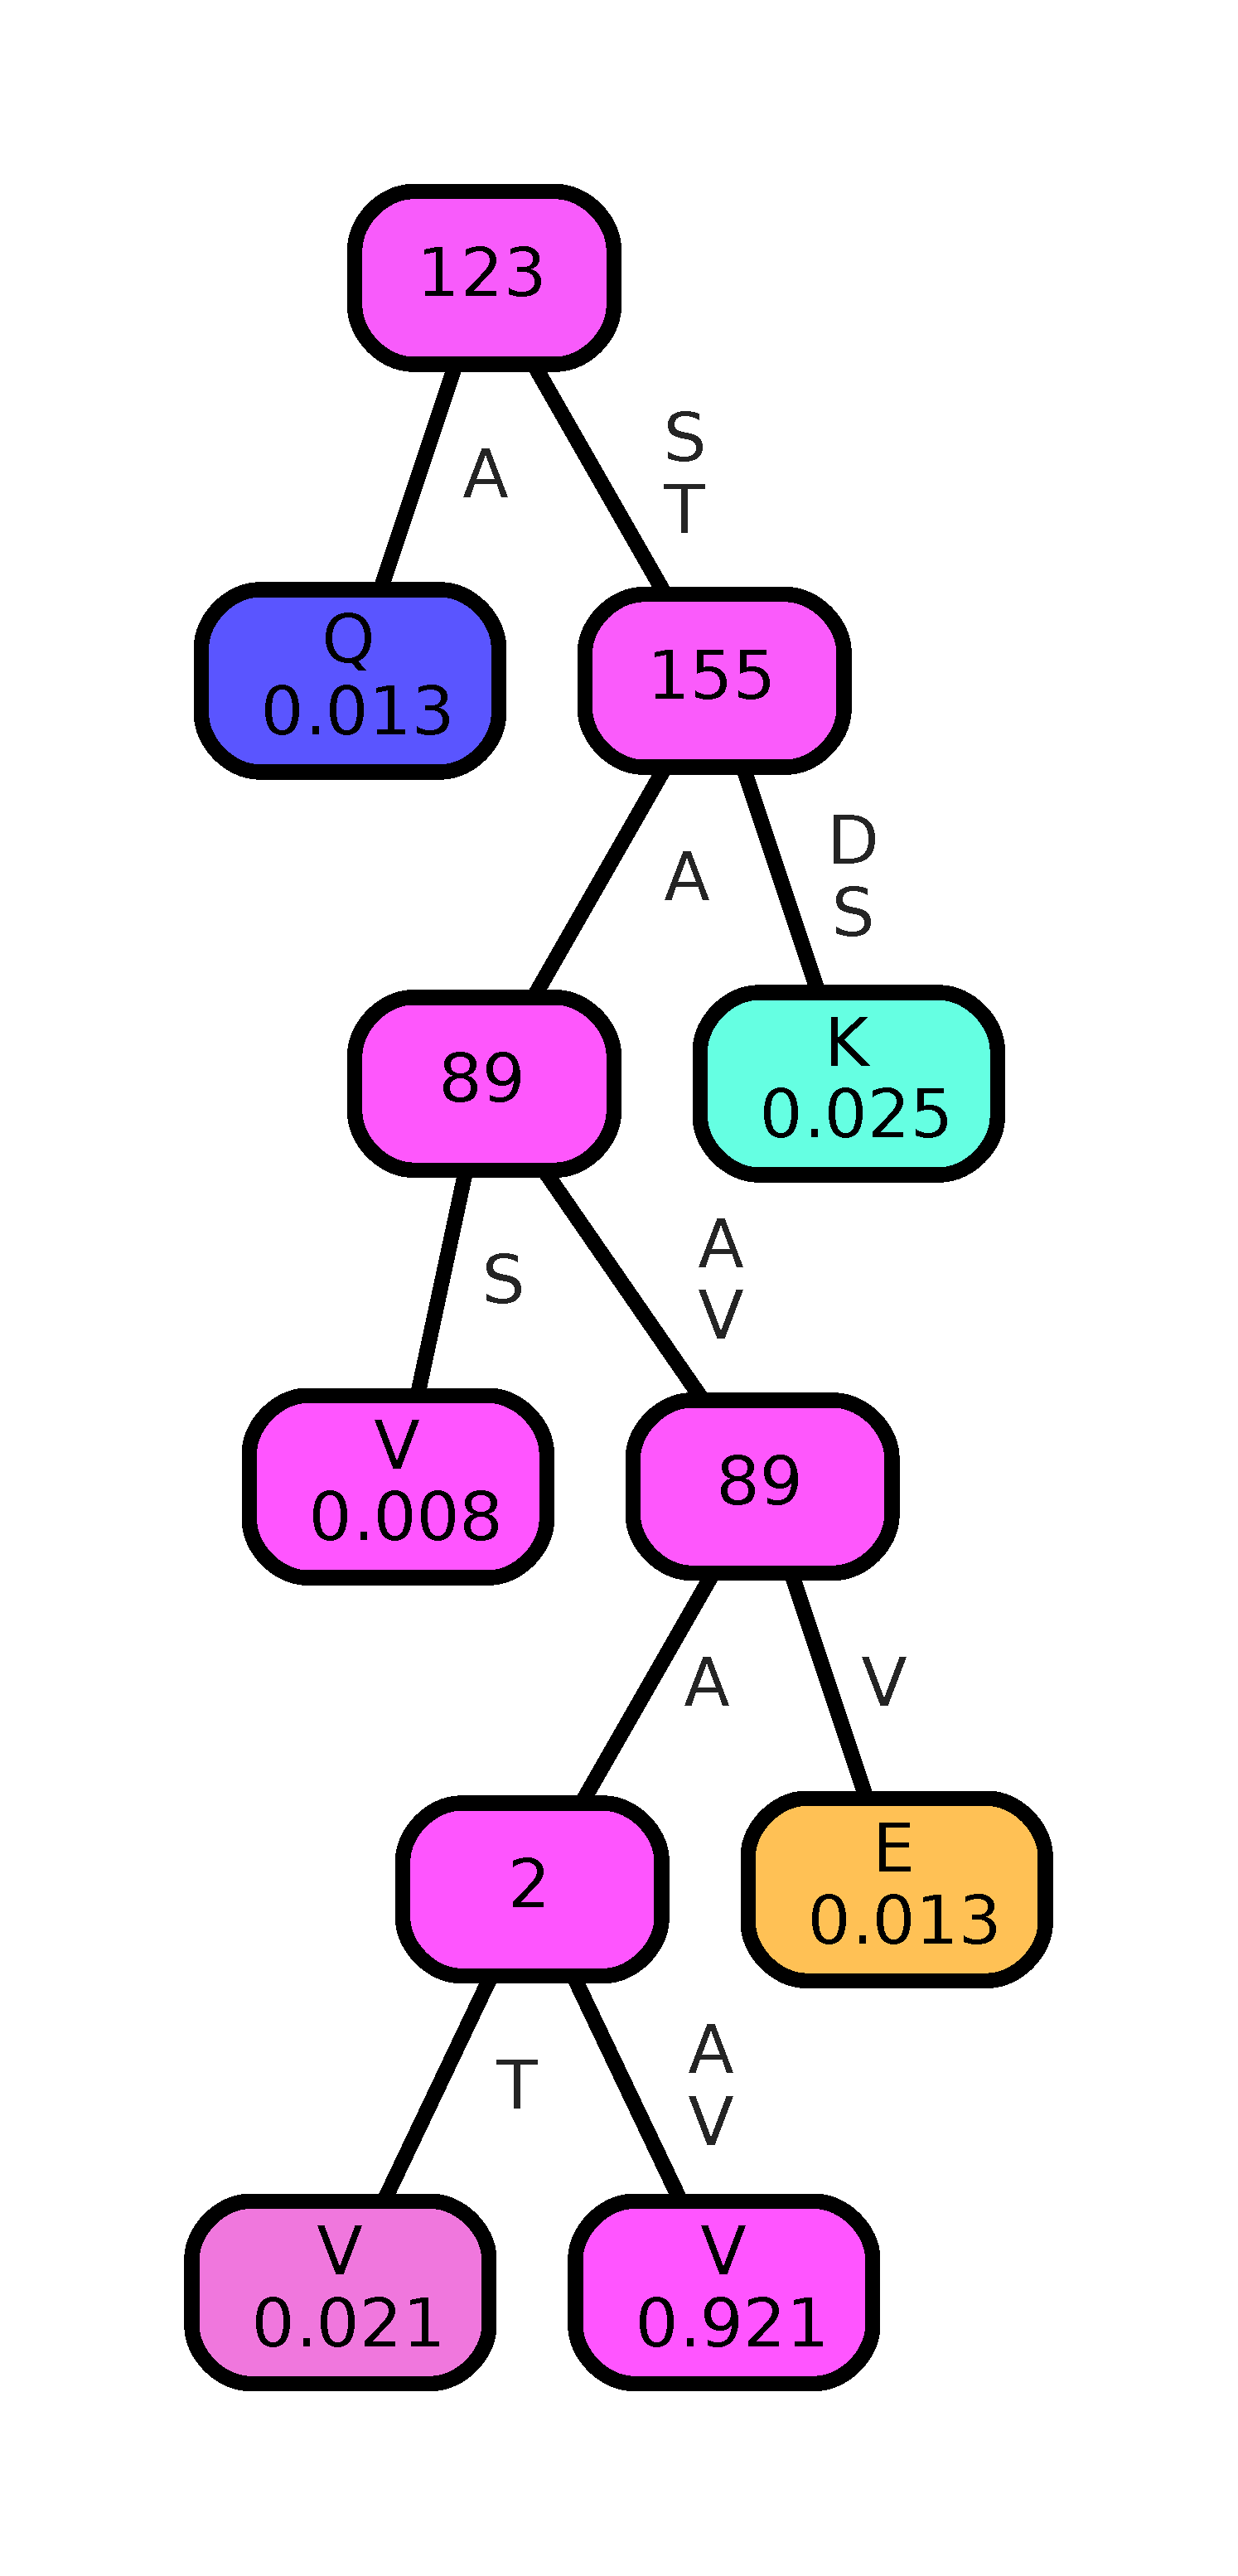
\includegraphics[width=\WDTB]{../qnet_predictions/qnet_models/trees/proc63}}; 

      
      \node[anchor=north,xcirc,inner sep=-20pt,label={[xshift=-.6in,yshift=.7in,align=center,\LCOL]-90:index\\155}] (P155) at (Z) {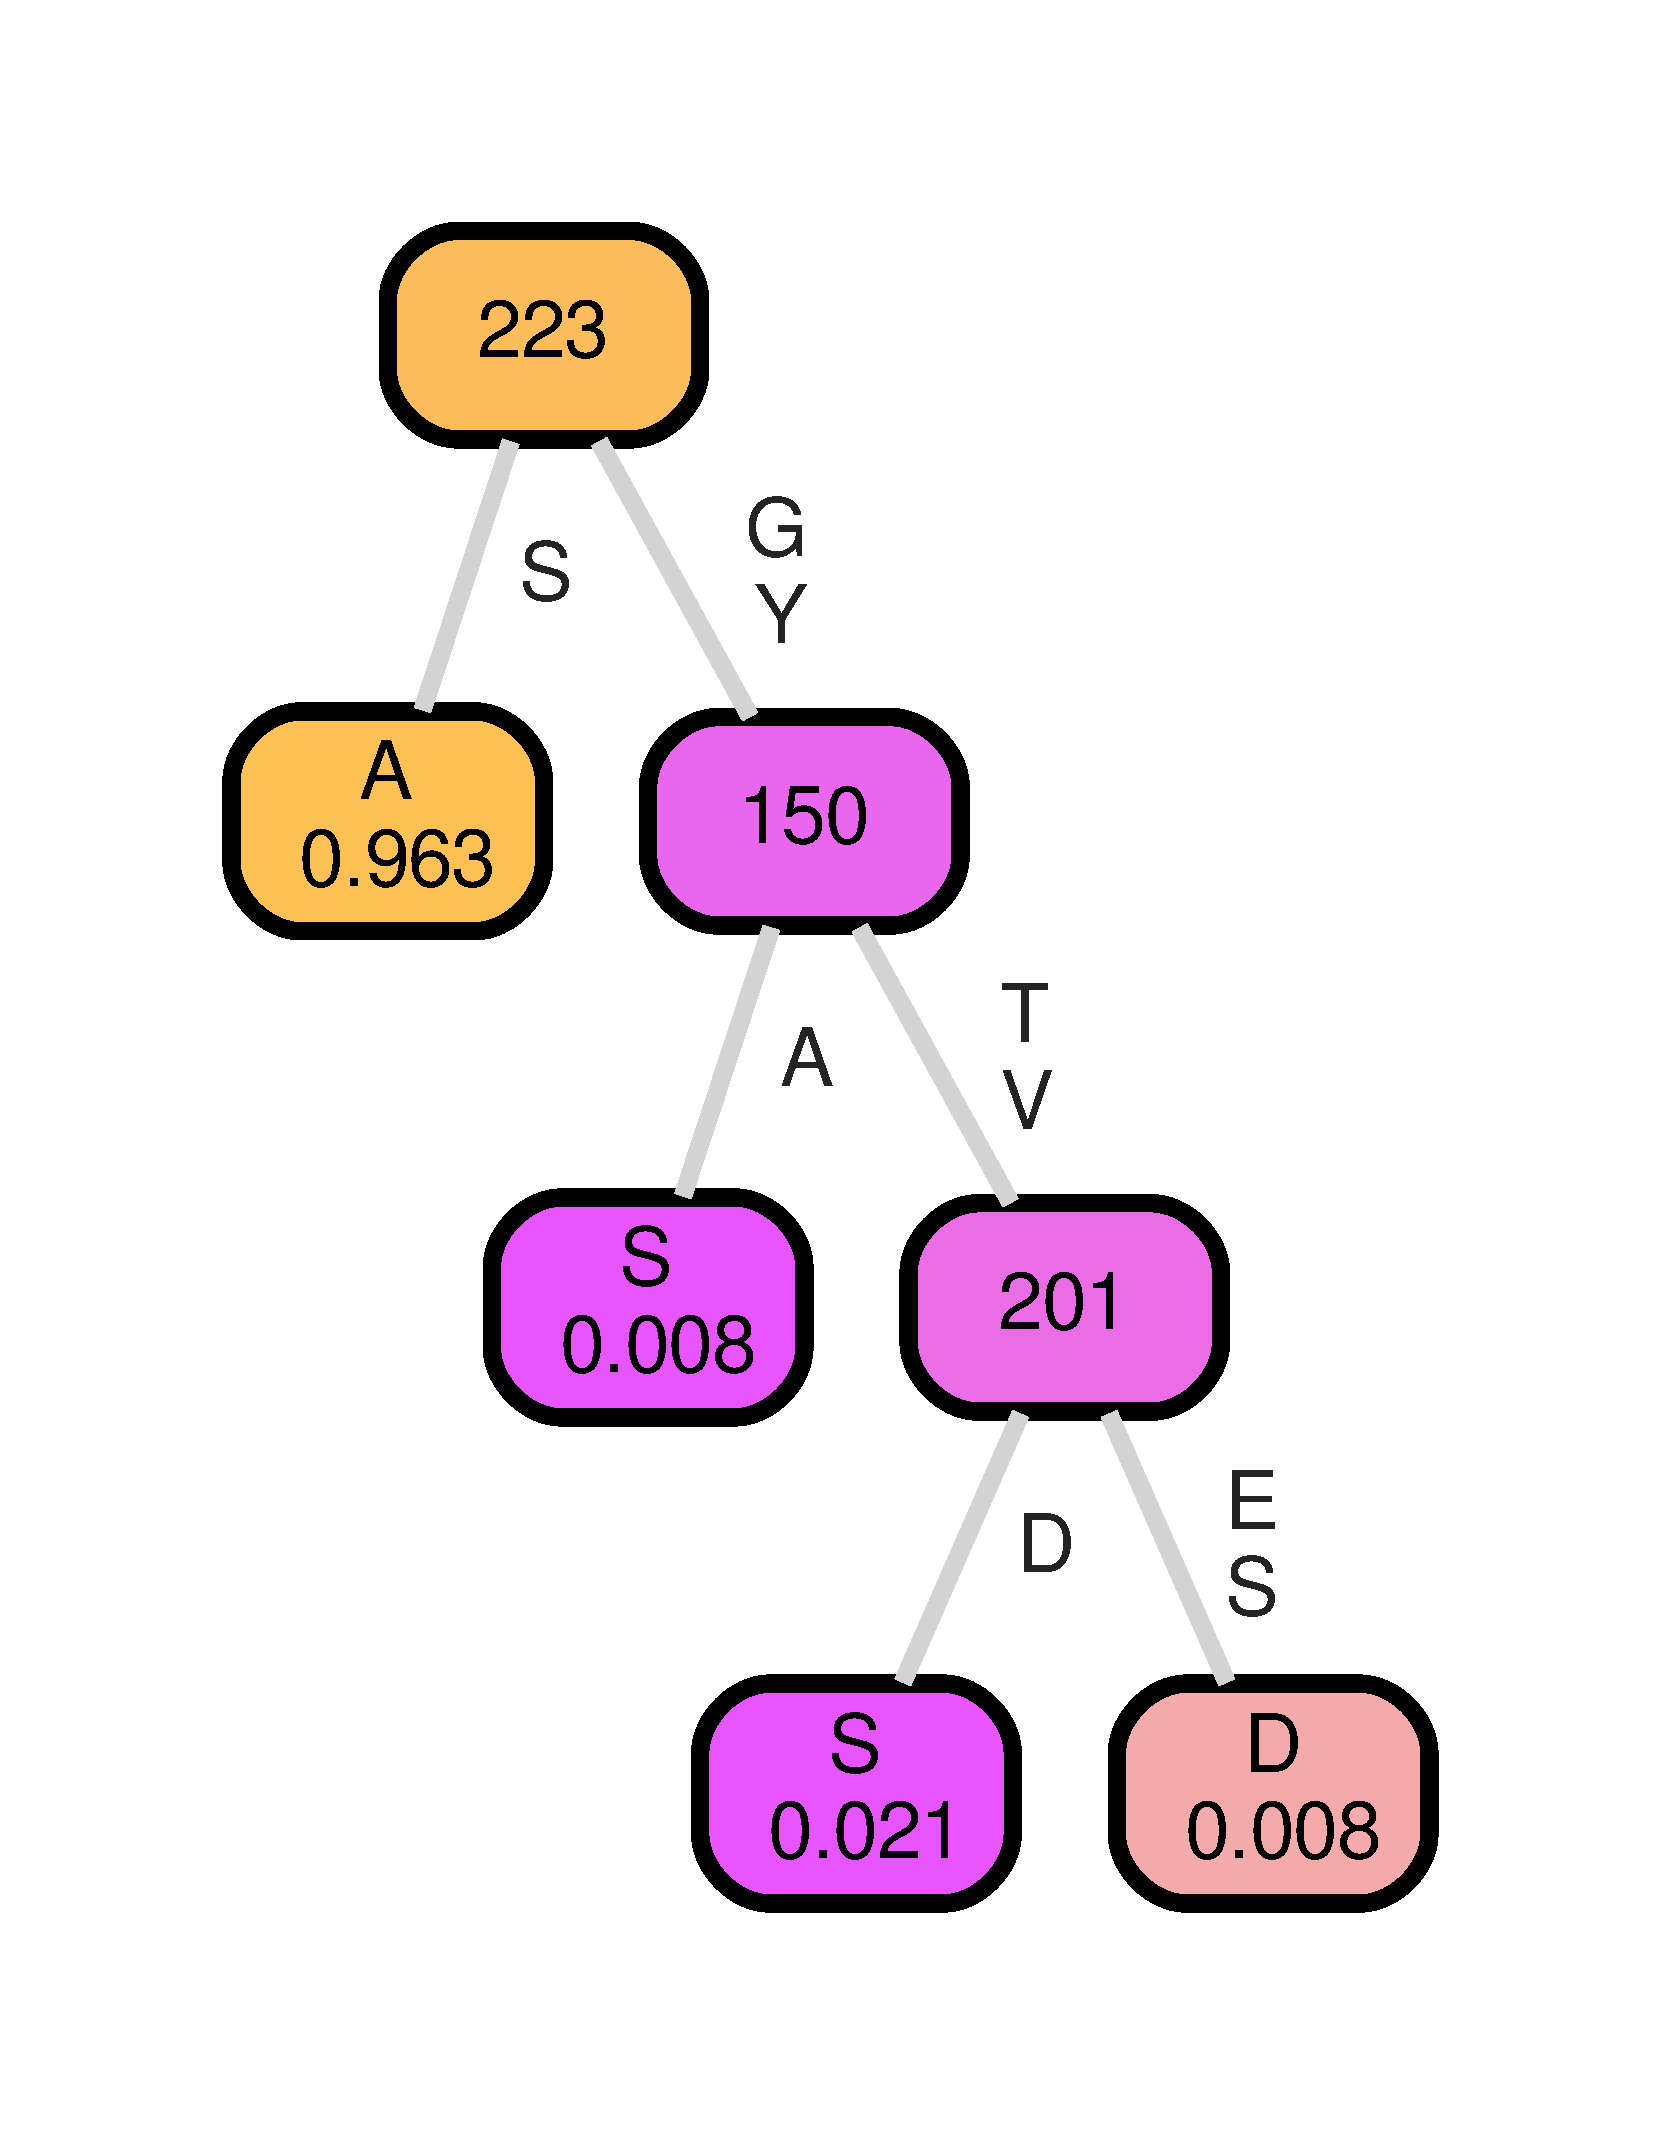
\includegraphics[width=\WDTC]{../qnet_predictions/qnet_models/trees/proc155}};

      \node[anchor=north,xcirc,inner sep=-25pt,label={[yshift=.65in,xshift=-.45in,align=center,\LCOL]-90:index\\14}] (P14) at ([xshift=-2.2in,yshift=-0.8in]P155.south) {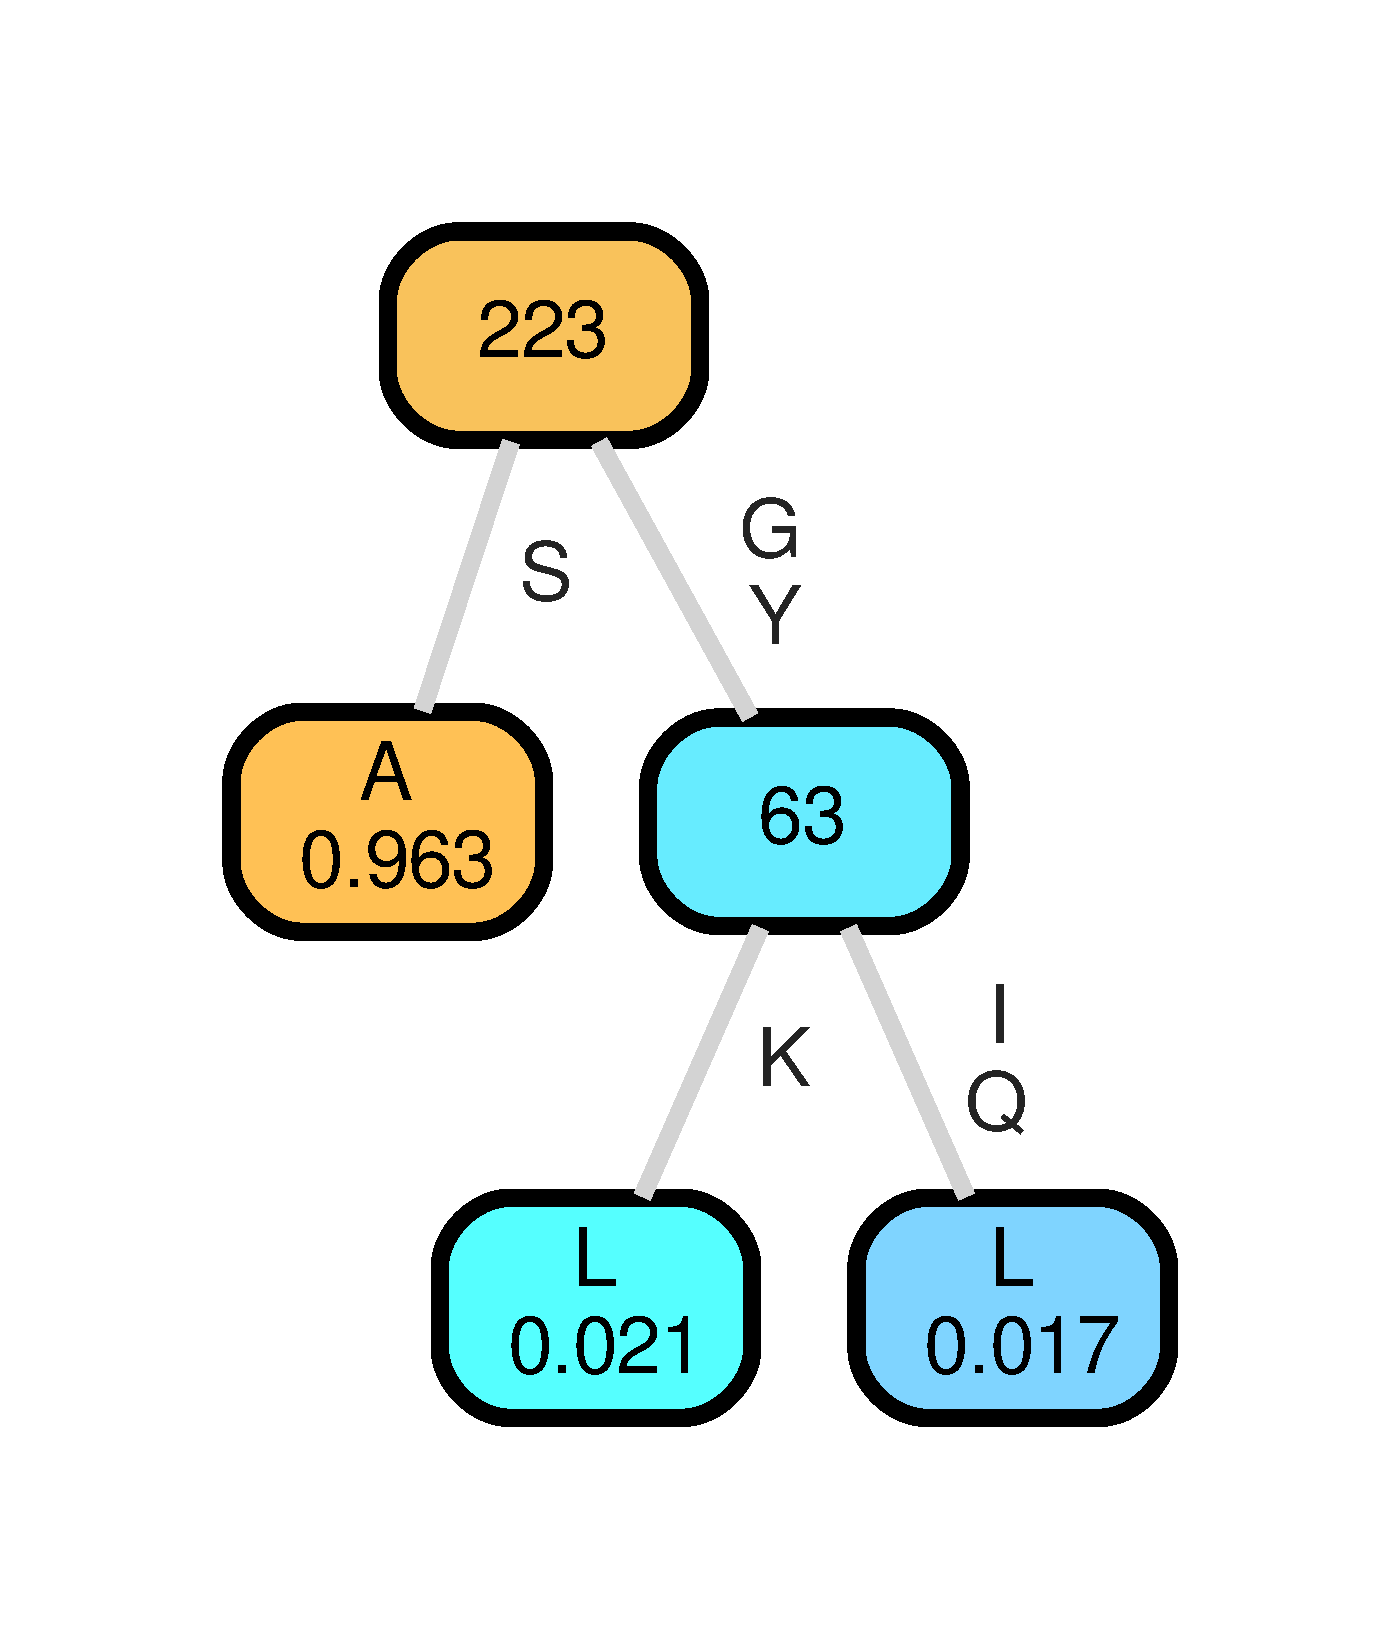
\includegraphics[width=\WDTB]{../qnet_predictions/qnet_models/trees/proc14}}; 
      
      \node[anchor=north,xcirc,inner sep=-25pt,label={[yshift=.6in,xshift=-.5in,align=center,\LCOL]-90:index\\223}] (P223) at ([xshift=-0in,yshift=-0.10in]P155.south) {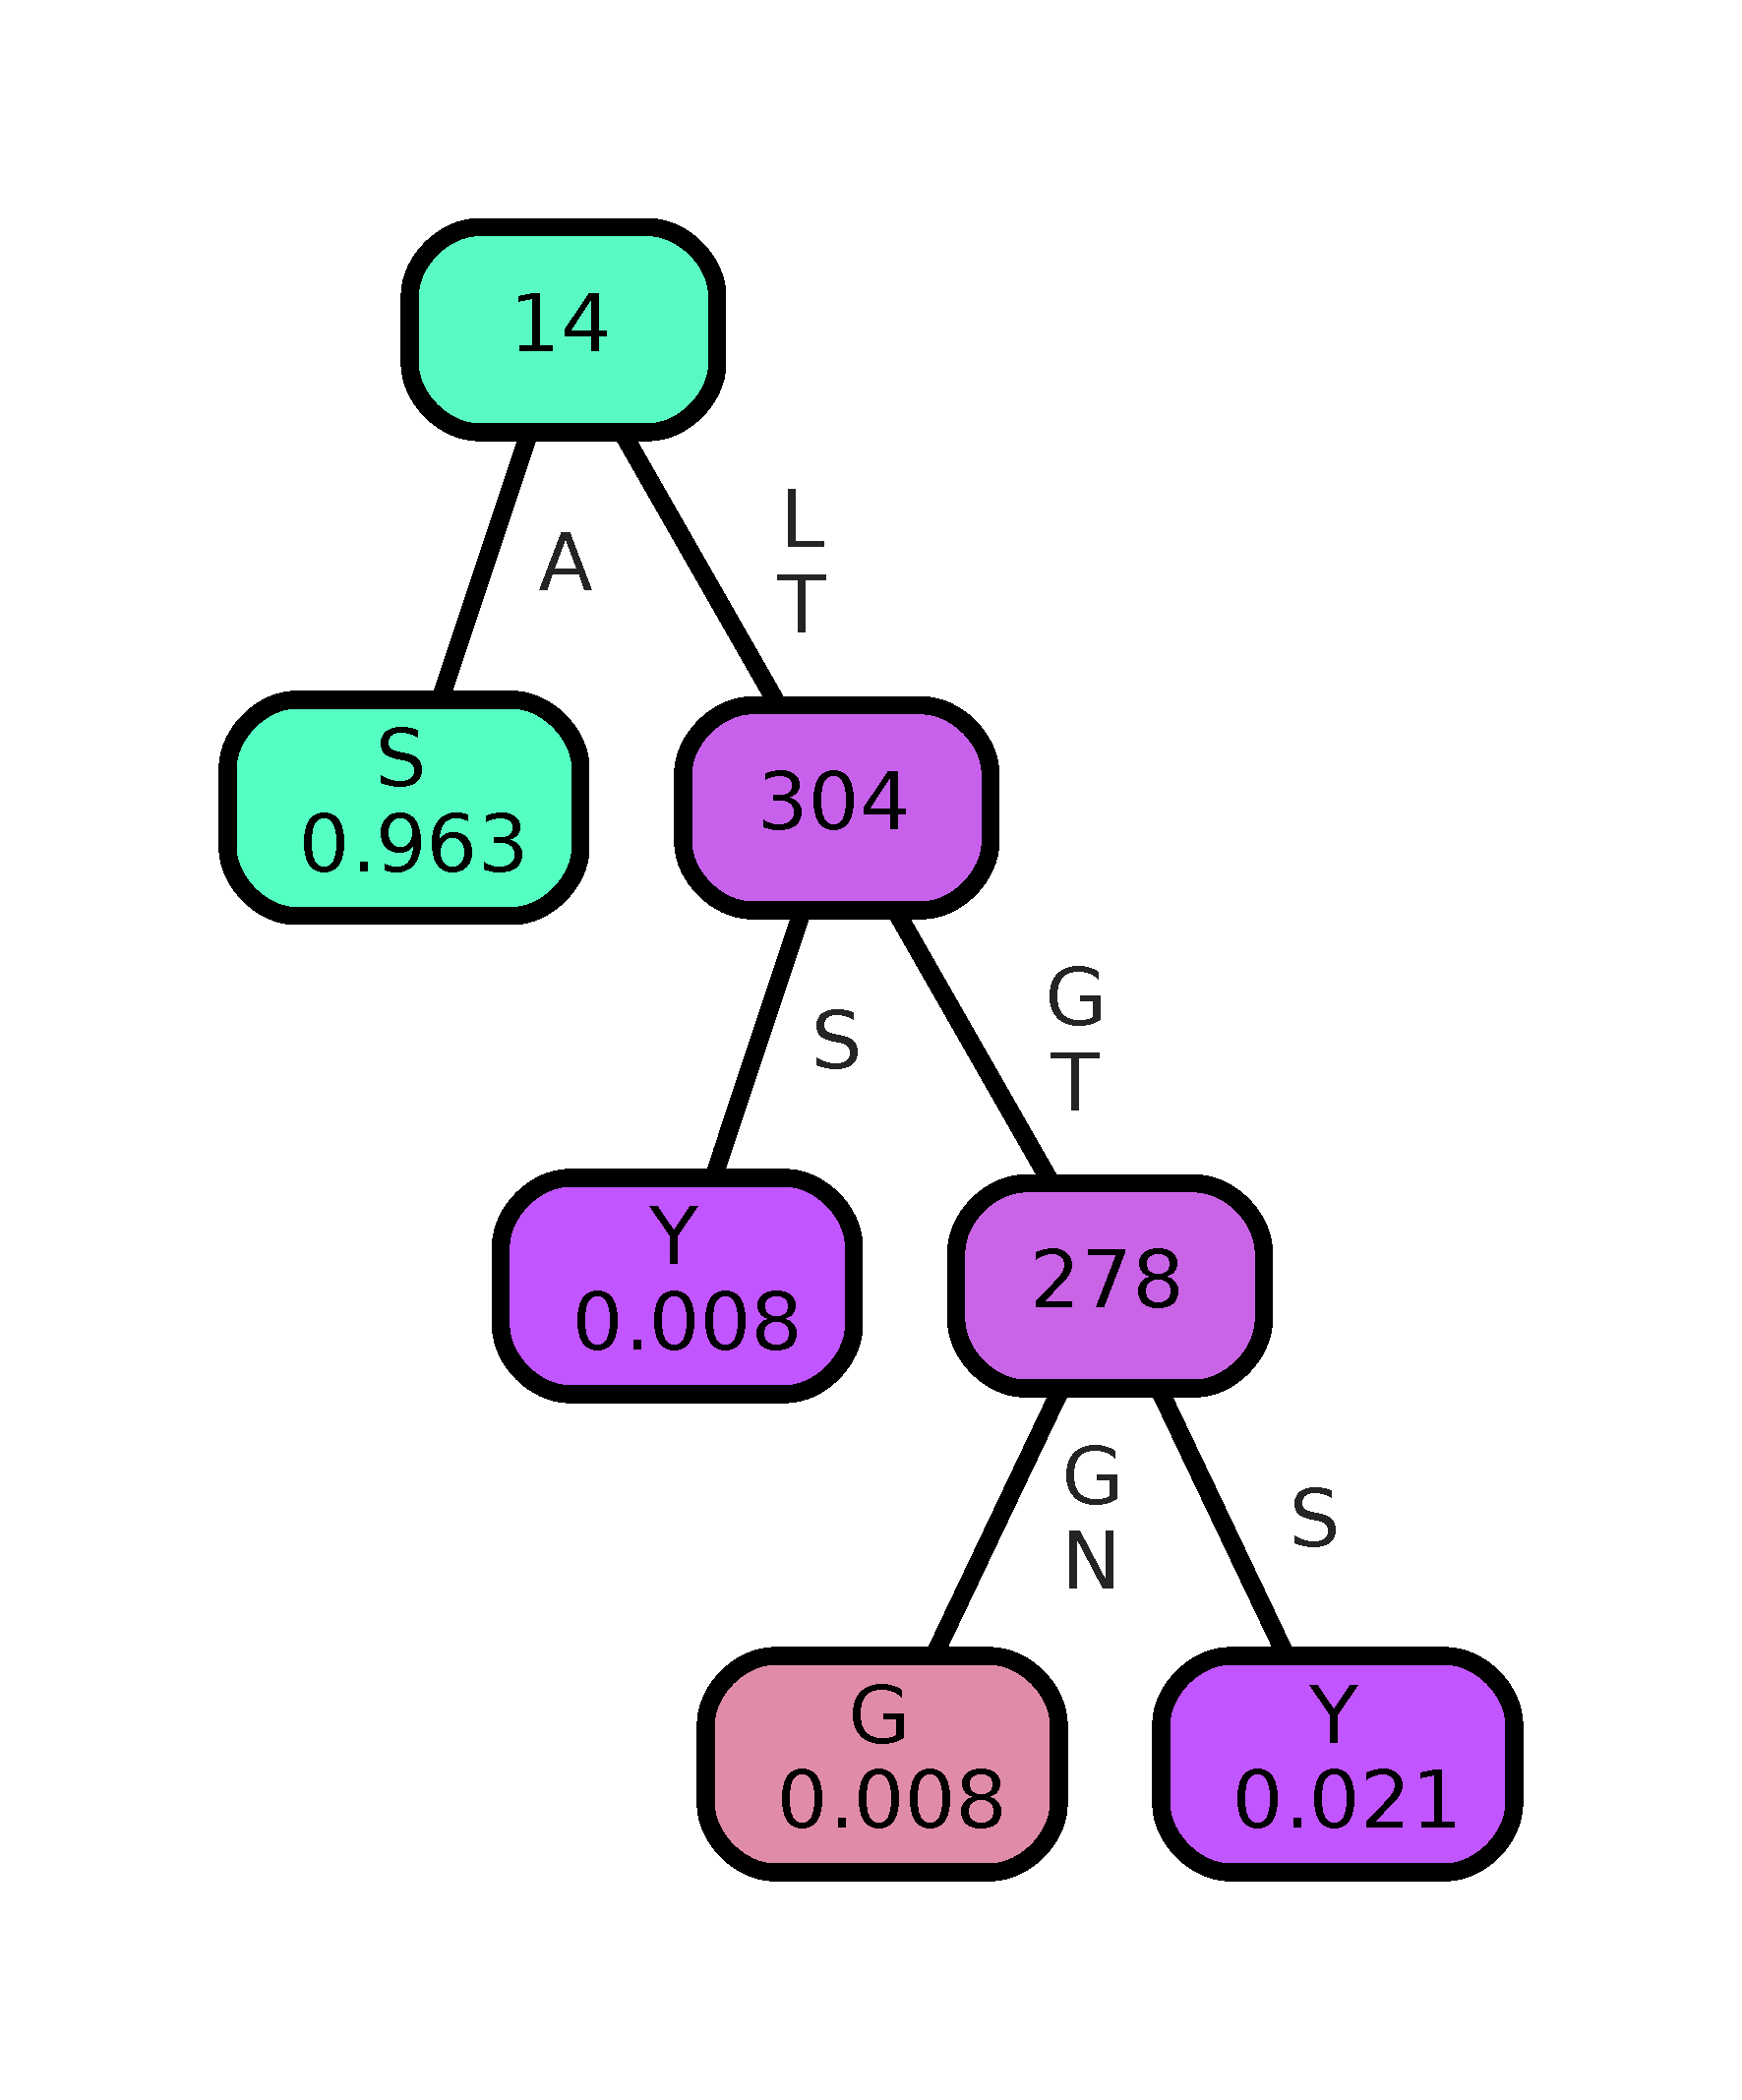
\includegraphics[width=\WDT]{../qnet_predictions/qnet_models/trees/proc223}};


      \node[text width=.13in,  rounded corners=8pt, line width=2pt,,inner sep=10pt,opacity=1,draw=\DCOLx] (X1) at ([yshift=.835in,xshift=.12in]P63) {};
      \draw [line width=\LWT,\DCOLx,-latex,] (X1)  to [out=75,in=140,looseness=1.55]  (P155);

      \node[text width=.13in,  rounded corners=8pt, line width=2pt,inner sep=10pt,opacity=1,draw=\DCOLx] (X2) at ([yshift=.845in,xshift=-.335in]P155) {};
      \draw [line width=\LWT,\DCOLx,-latex,] (X2)  to [out=0,in=60,looseness=1]  (P223);

      \node[text width=.13in,  rounded corners=8pt, line width=2pt,,inner sep=10pt,opacity=1,draw=\DCOLx] (X3) at ([yshift=.0in,xshift=.12in]P14) {};
      \draw [line width=\LWT,\DCOLx,-latex,] (X3)  to [out=150,in=-120,looseness=1.1]  (P63);

      \node[text width=.15in,  rounded corners=8pt, line width=2pt,inner sep=10pt,opacity=1,draw=\DCOLx] (X4) at ([yshift=.88in,xshift=-.34in]P223) {};
      \draw [line width=\LWT,\DCOLx,-latex,] (X4)  to [out=210,in=35,looseness=1.2]  (P14);

      \node[anchor=north,align=left,font=\bf\tt\footnotesize] (N3) at ([yshift=-6.1in,xshift=-1.85in]Z.south) {\bf\sffamily\fontsize{7}{8}\selectfont H1N1 2020-2021\\\bf\sffamily\fontsize{7}{8}\selectfont Haemagglutinin Sequences\\$\cdots$GTSRY{\color{Red1}S}KKFKPEIATRPKVRDQEGR$\cdots$\\$\cdots$GTSKY{\color{Red1}G}KKFMPEIARRPKVRNQEGR$\cdots$\\
        $\cdots$GSSKY{\color{Red1}Y}KRFTPEIVARPKVREQAGR$\cdots$\\
 $\cdots$GSSKY{\color{Red1}Y}KRFTPEIVARPKVREQAGR$\cdots$};

%A/Niger/8327/2020 
%
%A/Parana/10835/2021
%A/Gansu-Xifeng/1143/2021
%A/Sichuan/01208/2021

   \node[anchor=west,align=left,font=\bf\sffamily\fontsize{8}{10}\selectfont] (N4) at ([xshift=0.1in,yshift=.05in]N3.east) {A/Niger/8327/2020 \\
    A/Parana/10835/2021\\
      A/Gansu-Xifeng/1143/2021\\  
      A/Sichuan/01208/2021};

       \draw [ultra thick] ([yshift=.25in,xshift=.01in]N4.west) --++ (-.13in,-.190in);
       \draw [ultra thick] ([yshift=.1in,xshift=.01in]N4.west) --++ (-.13in,-.2in);
       \draw [ultra thick] ([yshift=-0.05in,xshift=.01in]N4.west) --++ (-.13in,-.2in);
       \draw [ultra thick] ([yshift=-.2in,xshift=.01in]N4.west) --++ (-.13in,-.2in);

       \node [align=center,text=IndianRed2,anchor=north] at ([xshift=-2.25in,yshift=-.1in]N4.south) {index 223};

      \node[anchor=west,rounded corners=3pt,align=center] (I1) at ([yshift=-.6in,xshift=.3in]P14.south west) {Color key (mixed colors represent distributions)};


      \definecolor{Acol}{RGB}{255,193,85}
      \definecolor{Dcol}{RGB}{255,255,85}
      \definecolor{Ecol}{RGB}{255,255,85}
      \definecolor{Gcol}{RGB}{136,255,85}
      \definecolor{Icol}{RGB}{85,255,150}
      \definecolor{Kcol}{RGB}{85,255,255}
      \definecolor{Lcol}{RGB}{85,255,255}
      \definecolor{Qcol}{RGB}{111,85,255}
      \definecolor{Scol}{RGB}{231,85,255}
      \definecolor{Tcol}{RGB}{255,85,255}
      \definecolor{Vcol}{RGB}{255,85,255}
      \definecolor{Ycol}{RGB}{255,85,97}
      
      \node[font=\bf\sffamily,anchor=north,rounded corners=3pt,text width=.1in,text height=.1in,fill=Acol,align=center,opacity=\OPC] (I1) at ([yshift=-.05in]I1.south west) {A};
      \node[font=\bf\sffamily,anchor=west,rounded corners=3pt,text width=.1in,text height=.1in,fill=Dcol,align=center,opacity=\OPC] (I1) at ([xshift=.05in]I1.east) {D};
      \node[font=\bf\sffamily,anchor=west,rounded corners=3pt,text width=.1in,text height=.1in,fill=Ecol,align=center,opacity=\OPC] (I1) at ([xshift=.05in]I1.east) {E};
      \node[font=\bf\sffamily,anchor=west,rounded corners=3pt,text width=.1in,text height=.1in,fill=Gcol,align=center,opacity=\OPC] (I1) at ([xshift=.05in]I1.east) {G};
      \node[font=\bf\sffamily,anchor=west,rounded corners=3pt,text width=.1in,text height=.1in,fill=Icol,align=center,opacity=\OPC] (I1) at ([xshift=.05in]I1.east) {I};
      \node[font=\bf\sffamily,anchor=west,rounded corners=3pt,text width=.1in,text height=.1in,fill=Kcol,align=center,opacity=\OPC] (I1) at ([xshift=.05in]I1.east) {K};
      \node[font=\bf\sffamily,anchor=west,rounded corners=3pt,text width=.1in,text height=.1in,fill=Lcol,align=center,opacity=\OPC] (I1) at ([xshift=.05in]I1.east) {L};
      \node[font=\bf\sffamily,anchor=west,rounded corners=3pt,text width=.1in,text height=.1in,fill=Qcol,align=center,opacity=\OPC] (I1) at ([xshift=.05in]I1.east) {Q};
      \node[font=\bf\sffamily,anchor=west,rounded corners=3pt,text width=.1in,text height=.1in,fill=Scol,align=center,opacity=\OPC] (I1) at ([xshift=.05in]I1.east) {S};
      \node[font=\bf\sffamily,anchor=west,rounded corners=3pt,text width=.1in,text height=.1in,fill=Tcol,align=center,opacity=\OPC] (I1) at ([xshift=.05in]I1.east) {T};
      \node[font=\bf\sffamily,anchor=west,rounded corners=3pt,text width=.1in,text height=.1in,fill=Vcol,align=center,opacity=\OPC] (I1) at ([xshift=.05in]I1.east) {V};
      \node[font=\bf\sffamily,anchor=west,rounded corners=3pt,text width=.1in,text height=.1in,fill=Ycol,align=center,opacity=\OPC] (I1) at ([xshift=.05in]I1.east) {Y};

      % \node[font=\bf\sffamily,anchor=north,rounded corners=3pt,text width=.1in,text height=.1in,fill=DarkOrange3!70,align=center,opacity=\OPC] (I1) at ([yshift=-.05in]I1.south) {A};

      % \node[font=\bf\sffamily,anchor=north,rounded corners=3pt,text width=.1in,text height=.1in,fill=SeaGreen2,align=center,opacity=\OPC] (I1) at ([yshift=-.05in]I1.south) {C};

      % \node[font=\bf\sffamily,anchor=north,rounded corners=3pt,text width=.1in,text height=.1in,fill=DodgerBlue2!80,align=center,opacity=\OPC] (I1) at ([yshift=-.050in]I1.south) {G};
    \end{tikzpicture}
  };

  \node [anchor=south west] (L1) at ([yshift=-.2650in]T.north west) {\Large a.};
  \node [anchor=south west] (L2) at ([yshift=-3.25in]T.north west) {\Large c.};
  \node [anchor=south west] (L3) at ([yshift=-5.65in]T.north west) {\Large d.};

\end{tikzpicture}

 \else
  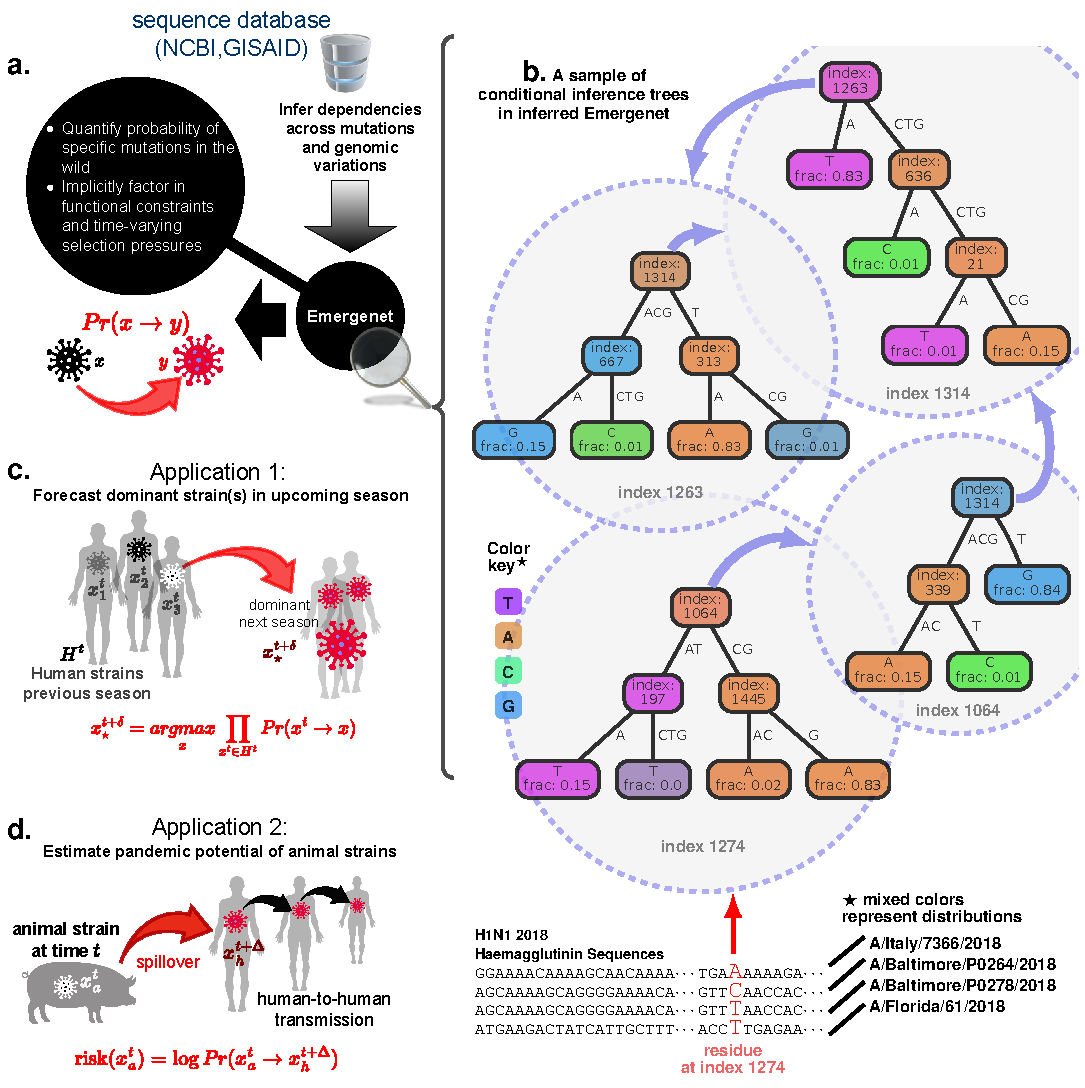
\includegraphics[width=\textwidth]{Figures/External/scheme}
  \fi
  \vspace{-20pt}
  
 \captionN{\textbf{\enet inference and applications}. \textbf{a}, Variations of
   genomes for identical subgroups of \infl are analyzed to infer a recursive forest of conditional inference trees~\cite{Hothorn06unbiasedrecursive} -- the \enet --   which maximally captures the emergent  dependencies between an a priori unspecified number of   mutations, deletions and insertions. With these inferred dependencies we can    estimate the numerical odds of specific mutations, and by extension, the numerical value of
   the probability of one strain giving rise to another in the wild, under  complex selection pressures from the background. b, Snapshot of decision trees  from the
   \enet constructed for H1N1 haemagglutinnin 2018 sequences. Note that the decision tree predicting the bases at index 1274   uses the bases at 1064, 1445, 197 as features. These features are automatically selected, as being maximally predictive  of the bases be at 1274. Then, we compute predictors for each of these  feature indices, $e.g.$   trees for  index 1064, which involves index 1314 and 339 as features. Continuing, we find that the trees for index 1314 involves indices 1263, 636 and 21, and that for 1263 involves 1314, 667 and 313. The predictor for 1263  depends on 1314, and that for 1314 depends on 1263, revealing the recursive structure of \enet. c, First application: With \enet induced ability to quantify mutation probabilities,  we forecast  dominant strain(s) for the next flu season, using only  sequences collected in the previous season (and the inferred \enet, using data from the past year). d, Second application: estimation of the risk of a global pandemic posed by individual animal strains that are still not known to circulate in humans.}\label{figscheme}.
\end{figure*}
\else
\refstepcounter{figure}\label{figscheme}
\fi  
%#############################################                                  
%#############################################                                  
%#############################################
%#############################################
\ifFIGS
\begin{figure*}[!ht]
  \centering
  \tikzexternalenable
   \tikzsetnextfilename{seasonalpred_both}

  \tikzXtrue 
  \iftikzX
  \hspace{-20pt}\resizebox{.975\linewidth}{!}{\begin{tikzpicture}
  \def\HGT{.35in}
  \def\WDT{2.75in}
  \def\YST{-.3in}

  \node[,label={[font=\bf\sffamily,yshift=-.60in]90:\underline{Southern Hemisphere (Prediction in December)}}] (AAA) at (0,0) {\pgfplotsset{
  discard if/.style 2 args={
    x filter/.append code={
      \edef\tempa{\thisrow{#1}}
      \edef\tempb{#2}
      \ifx\tempa\tempb
      \def\pgfmathresult{inf}
      \fi
    }
  },
  discard if not/.style 2 args={
    x filter/.append code={
      \edef\tempa{\thisrow{#1}}
      \edef\tempb{#2}
      \ifx\tempa\tempb
      \else
      \def\pgfmathresult{inf}
      \fi
    }
  }
}

\begin{tikzpicture}

  \def\NNX{1}
  \noexpand\def\YMAX{15}
  \def\YLABEL{}
  \newcommand{\PPX}[3][2001]{
    \begin{axis}[name=XX,\TEXTCOL,anchor=center,
      title={},legend columns=1,
      legend style={text=black,anchor=west,at={(0.5,1.8)},
        inner sep=1pt,draw=none,fill=black!5,fill opacity=.75,align=right,
        text opacity=1,/tikz/column 2/.style={
          column sep=5pt,
        },},
      ymax=0,
      ymin=-\YMAX,
      xmin=#1,
      xmax=2022,
      name=X0,
      anchor=center,
      width=\WDT,
      height=\HGT,
      scale only axis=true,
      enlargelimits=false,
      enlarge y limits=false,
      enlarge x limits=0.06,
      axis on top=false,
      axis line style={black!2, very thick},
      grid=both,minor x tick num=3,
      major grid style={opacity=1,,thick,black!10},
      minor grid style={opacity=1,,semithick,Red4!5},
      major tick length=0pt,
      minor tick length=0pt,
      ytick style={draw=none},
      scaled y ticks = false,
      y tick label style={/pgf/number format/fixed,
        /pgf/number format/1000 sep = \empty % \thinspace optional
      },
      x tick label style={/pgf/number format/fixed,
        /pgf/number format/1000 sep = \empty % Optional
      },
      xlabel={year},ylabel style={yshift=1in,align=center,xshift=1.9in},
      xlabel style={yshift=.05in},ybar,,bar width=\BWIDTH,
      ytick={#2},xtick={2000,2004,2008,2012,2016,2020},xticklabels={},xlabel={},ylabel={\YLABEL},,ylabel style={yshift=-.8in,align=center,xshift=-1.9in},
      xtick=data, xticklabel style={rotate=90}]
      
      \addplot [area legend,restrict x to domain=0:2022,negstyle]
      table [col sep=comma,x expr=\coordindex+#1,
      y expr=(\thisrow{\NMX}
      -\thisrow{ldistance_WHO})/(\NNX)] {\DATAQNETx};
    \end{axis}
    % 
    \begin{axis}[\TEXTCOL,anchor=center,yshift=\HGT,
      title={},legend columns=1,legend style={text=black,anchor=west,at={(0.5,.8)},
        inner sep=1pt,draw=none,fill=black!5,fill opacity=.75,align=right,
        text opacity=1,/tikz/column 2/.style={
          column sep=5pt,
        },},
      ymin=0,
      ymax=\YMAX,
      xmax=2022,
      xmin=#1,
      name=X0,
      anchor=center,
      width=\WDT,
      height=\HGT,
      scale only axis=true,
      enlargelimits=false,
      enlarge y limits=false,
      enlarge x limits=0.06,
      axis on top=false,
      axis line style={black!2, very thick},
      grid=both,minor x tick num=3,
      major grid style={opacity=1,,thick,black!10},
      minor grid style={opacity=1,,semithick,Red4!5},
      major tick length=0pt,
      minor tick length=0pt,
      ytick style={draw=none},
      scaled y ticks = false,
      y tick label style={/pgf/number format/fixed,
        /pgf/number format/1000 sep = \empty % \thinspace optional
      },
      x tick label style={/pgf/number format/fixed,
        /pgf/number format/1000 sep = \empty % Optional
      },
      xlabel={year},ylabel style={yshift=0.8in,align=center,xshift=1in},
      xlabel style={yshift=.05in},ybar,,bar width=\BWIDTH,ytick={#3},,xtick={2000,2004,2008,2012,2016,2020},xticklabels={},xlabel={},
      xtick=data, xticklabel style={rotate=90}]
      
      \addplot [area legend,restrict x to domain=0:2022,posstyle]
      table [col sep=comma,x expr=\coordindex+#1,y expr=(\thisrow{\NMX}-\thisrow{ldistance_WHO})/(\NNX)] {\DATAQNETx};
    \end{axis}

    \begin{axis}[\TEXTCOL,anchor=center,yshift=0,
      title={},legend columns=1,legend style={text=black,anchor=west,at={(0.5,.8)},
        inner sep=1pt,draw=none,fill=black!5,fill opacity=.75,align=right,
        text opacity=1,/tikz/column 2/.style={
          column sep=5pt,
        },},
      ymin=0,
      ymax=\YMAX,
      xmax=2022, 
      xmin=#1,
      name=X0,
      anchor=center,
      width=\WDT,
      height=\HGT,
      scale only axis=true,
      enlargelimits=false,
      enlarge y limits=false,
      enlarge x limits=0.060,
      axis on top=false,
      axis line style={black!2, very thick},
      % grid,
      grid style={opacity=1,dashed,thick,black!10},
      major tick length=0pt,
      ytick style={draw=none},
      scaled y ticks = false,
      y tick label style={/pgf/number format/fixed,
        /pgf/number format/1000 sep = \empty % \thinspace optional
      },
      x tick label style={/pgf/number format/fixed,
        /pgf/number format/1000 sep = \empty % Optional
      },
      xlabel={year},ylabel style={yshift=0.2in,align=center,xshift=1in},
      xlabel style={yshift=.05in},ybar,
      ,bar width=\BWIDTH,ytick={},yticklabels={},
      ,xtick={2000,2004,2008,2012,2016,2020},xlabel={},
      xtick=data, xticklabel style={rotate=90}]
      
      \addplot [area legend,restrict x to domain=0:2022,draw=none,fill=none]
      table [col sep=comma,x expr=\coordindex+#1,y expr=0] {\DATAQNETx};
    \end{axis}
  }

  \def\TEXTCOL{gray}
  \def\RCLR{IndianRed1}
  \def\RCLRB{IndianRed1}
  \def\QCLRC{Orchid3}
  \def\QCLD{gray!50}
  \def\QCLRB{black}
  \def\QCLR{black}
  \def\YST{-.3in}
  \noexpand\def\PCOL{black!0}
  \noexpand\def\NCOL{black!0}
  \noexpand\def\PCOLf{black!90}
  \noexpand\def\NCOLf{Red1}
  \def\SC{1.35}
  \def\XCOL{lightgray!70}
  \def\BWIDTH{8.2pt}
  \tikzset{%
    posstyle/.style =   {line width=1pt,
      draw=\PCOL,fill=\PCOLf}}
  \tikzset{%
    negstyle/.style =   {line width=1pt,
      draw=\NCOL,fill=\NCOLf}}
  \def\HGT{.3in}
  \def\WDT{2.75in}

  \def\YTICKA{0,-5,-10}
  \def\YTICKB{0,5,10}
\def\NMX{ldistance_Qnet_recommendation}
  \node[anchor=north west] (A) at (0,0) {\begin{tikzpicture}[anchor=center,font=\bf\sffamily\fontsize{8}{9}\selectfont]
      \def\DATAQNETx{Figures/plotdata/south_h1n1_ha.csv}
      \def\YLABEL{}
      \PPX[2001]{\YTICKA}{\YTICKB}
    \end{tikzpicture}};

  \node[anchor=north west] (B) at ([yshift=\YST]A.south west) {\begin{tikzpicture}[anchor=center,font=\bf\sffamily\fontsize{8}{9}\selectfont]
      \def\DATAQNETx{Figures/plotdata/south_h1n1_na.csv}
      \def\YLABEL{}
      \PPX[2001]{\YTICKA}{\YTICKB}
    \end{tikzpicture}};

  \node[anchor=north west] (C) at ([xshift=-.25in,yshift=0in]A.north east) {\begin{tikzpicture}[anchor=center,font=\bf\sffamily\fontsize{8}{9}\selectfont]
      \def\DATAQNETx{Figures/plotdata/south_h3n2_ha.csv}
      \def\YLABEL{}
      \PPX[2005]{\YTICKA}{\YTICKB}
    \end{tikzpicture}};

  \node[anchor=north west] (D) at ($(B.north west)!(C.west)!(B.north east)$) {\begin{tikzpicture}[anchor=center,font=\bf\sffamily\fontsize{8}{9}\selectfont]
      \def\DATAQNETx{Figures/plotdata/south_h3n2_na.csv}
      \def\YLABEL{}
      \PPX[2003]{\YTICKA}{\YTICKB}
    \end{tikzpicture}};

\def\NMX{ldistance_Qnet_recommendation_0}

  \node[anchor=north west] (E) at ([yshift=\YST]B.south west) {\begin{tikzpicture}[anchor=center,font=\bf\sffamily\fontsize{8}{9}\selectfont]
      \def\DATAQNETx{Figures/plotdata/south_h1n1_na_3cluster.csv}
      \def\YLABEL{}
      \PPX[2001]{\YTICKA}{\YTICKB}
    \end{tikzpicture}};



  \node[anchor=north west] (F) at ($(E.north west)!(D.west)!(E.north east)$) {\begin{tikzpicture}[anchor=center,font=\bf\sffamily\fontsize{8}{9}\selectfont]
      \def\DATAQNETx{Figures/plotdata/south_h3n2_na_3cluster.csv}
      \def\YLABEL{}
      \PPX[2003]{\YTICKA}{\YTICKB}
    \end{tikzpicture}};



  
  \node[anchor=south west] (L1) at ([yshift=0in,xshift=.55in]A.north west) {{\Large a.} Influenza A H1N1 HA};
  \node[anchor=south west] (L2) at ([xshift=0in]$(L1.north west)!(B.north)!(L1.south west)$) {{\Large b.} Influenza A H1N1 NA};
  \node[anchor=south west] (L3) at ([xshift=0.55in]$(L1.south west)!(C.west)!(L1.south east)$) {{\Large c.} Influenza A H3N2 HA};
  \node[anchor=south west] (L4) at ($(L2.south west)!(L3.west)!(L2.south east)$) {{\Large d.} Influenza A H3N2 NA};

  \node[anchor=south west] (L5) at ([xshift=0in]$(L2.north west)!(E.north)!(L2.south west)$) {{\Large e.} Influenza A H1N1 NA (multi-cluster)};
  \node[anchor=south west] (L4) at ($(L5.south west)!(L4.west)!(L5.south east)$) {{\Large f.} Influenza A H3N2 NA (multi-cluster)};



  
   \node[opacity=1,fill=\PCOLf,text width=.5in,text height=.05in,label={[text=\PCOLf,fill=white,font=\bf\sffamily\fontsize{9}{6}\selectfont]0:WHO better}] (X1) at ([yshift=1.2in]$(A.west)!.70!2:(C.west)$) {};
   \node[opacity=1,fill=\NCOLf,text width=.5in,text height=.05in,label={[text=\NCOLf,fill=white,font=\bf\sffamily\fontsize{9}{6}\selectfont]0:\enet better},anchor=north west] (X1) at ([xshift=1.2in]X1.north east) {};

\end{tikzpicture}
};
  \node[anchor=north,label={[font=\bf\sffamily]90:\underline{Northern Hemisphere (Prediction in February)}}] (BBB) at ([yshift=-.25in]AAA.south) {\pgfplotsset{
  discard if/.style 2 args={
    x filter/.append code={
      \edef\tempa{\thisrow{#1}}
      \edef\tempb{#2}
      \ifx\tempa\tempb
      \def\pgfmathresult{inf}
      \fi
    }
  },
  discard if not/.style 2 args={
    x filter/.append code={
      \edef\tempa{\thisrow{#1}}
      \edef\tempb{#2}
      \ifx\tempa\tempb
      \else
      \def\pgfmathresult{inf}
      \fi
    }
  }
}

\begin{tikzpicture}

  \def\NNX{1}
  \noexpand\def\YMAX{15}
  \def\YLABEL{}
  \newcommand{\PPX}[3][2001]{
    \begin{axis}[name=XX,\TEXTCOL,anchor=center,
      title={},legend columns=1,
      legend style={text=black,anchor=west,at={(0.5,1.8)},
        inner sep=1pt,draw=none,fill=black!5,fill opacity=.75,align=right,
        text opacity=1,/tikz/column 2/.style={
          column sep=5pt,
        },},
      ymax=0,
      ymin=-\YMAX,
      xmin=#1,
      xmax=2022,
      name=X0,
      anchor=center,
      width=\WDT,
      height=\HGT,
      scale only axis=true,
      enlargelimits=false,
      enlarge y limits=false,
      enlarge x limits=0.06,
      axis on top=false,
      axis line style={black!2, very thick},
      grid=both,minor x tick num=3,
      major grid style={opacity=1,,thick,black!10},
      minor grid style={opacity=1,,semithick,Red4!5},
      major tick length=0pt,
      minor tick length=0pt,
      ytick style={draw=none},
      scaled y ticks = false,
      y tick label style={/pgf/number format/fixed,
        /pgf/number format/1000 sep = \empty % \thinspace optional
      },
      x tick label style={/pgf/number format/fixed,
        /pgf/number format/1000 sep = \empty % Optional
      },
      xlabel={year},ylabel style={yshift=1in,align=center,xshift=1.9in},
      xlabel style={yshift=.05in},ybar,,bar width=\BWIDTH,
      ytick={#2},%xtick={2000,2004,2008,2012,2016,2020}
      ,xticklabels={},xlabel={},ylabel={\YLABEL},,ylabel style={yshift=-.8in,align=center,xshift=-1.9in},
      xtick=data, xticklabel style={rotate=90}]
      
      \addplot [area legend,restrict x to domain=0:2022,negstyle]
      table [col sep=comma,x expr=\coordindex+#1,
      y expr=(\thisrow{\NMX}
      -\thisrow{ldistance_WHO})/(\NNX)] {\DATAQNETx};
    \end{axis}
    % 
    \begin{axis}[\TEXTCOL,anchor=center,yshift=\HGT,
      title={},legend columns=1,legend style={text=black,anchor=west,at={(0.5,.8)},
        inner sep=1pt,draw=none,fill=black!5,fill opacity=.75,align=right,
        text opacity=1,/tikz/column 2/.style={
          column sep=5pt,
        },},
      ymin=0,
      ymax=\YMAX,
      xmax=2022,
      xmin=#1,
      name=X0,
      anchor=center,
      width=\WDT,
      height=\HGT,
      scale only axis=true,
      enlargelimits=false,
      enlarge y limits=false,
      enlarge x limits=0.06,
      axis on top=false,
      axis line style={black!2, very thick},
      grid=both,minor x tick num=3,
      major grid style={opacity=1,,thick,black!10},
      minor grid style={opacity=1,,semithick,Red4!5},
      major tick length=0pt,
      minor tick length=0pt,
      ytick style={draw=none},
      scaled y ticks = false,
      y tick label style={/pgf/number format/fixed,
        /pgf/number format/1000 sep = \empty % \thinspace optional
      },
      x tick label style={/pgf/number format/fixed,
        /pgf/number format/1000 sep = \empty % Optional
      },
      xlabel={year},ylabel style={yshift=0.8in,align=center,xshift=1in},
      xlabel style={yshift=.05in},ybar,,bar width=\BWIDTH,ytick={#3},,%xtick={2000,2004,2008,2012,2016,2020},
      xticklabels={},xlabel={},xtick=data, xticklabel style={rotate=90}]
      
      \addplot [area legend,restrict x to domain=0:2022,posstyle]
      table [col sep=comma,x expr=\coordindex+#1,y expr=(\thisrow{\NMX}-\thisrow{ldistance_WHO})/(\NNX)] {\DATAQNETx};
    \end{axis}

    \begin{axis}[\TEXTCOL,anchor=center,yshift=0,
      title={},legend columns=1,legend style={text=black,anchor=west,at={(0.5,.8)},
        inner sep=1pt,draw=none,fill=black!5,fill opacity=.75,align=right,
        text opacity=1,/tikz/column 2/.style={
          column sep=5pt,
        },},
      ymin=0,
      ymax=\YMAX,
      xmax=2022, 
      xmin=#1,
      name=X0,
      anchor=center,
      width=\WDT,
      height=\HGT,
      scale only axis=true,
      enlargelimits=false,
      enlarge y limits=false,
      enlarge x limits=0.060,
      axis on top=false,
      axis line style={black!2, very thick},
      % grid,
      grid style={opacity=1,dashed,thick,black!10},
      major tick length=0pt,
      ytick style={draw=none},
      scaled y ticks = false,
      y tick label style={/pgf/number format/fixed,
        /pgf/number format/1000 sep = \empty % \thinspace optional
      },
      x tick label style={/pgf/number format/fixed,
        /pgf/number format/1000 sep = \empty % Optional
      },
      xlabel={year},ylabel style={yshift=0.2in,align=center,xshift=1in},
      xlabel style={yshift=.05in},ybar,
      ,bar width=\BWIDTH,ytick={},yticklabels={},
      %,xtick={2000,2004,2008,2012,2016,2020},
      xlabel={},xtick=data, xticklabel style={rotate=90}]
      
      \addplot [area legend,restrict x to domain=0:2022,draw=none,fill=none]
      table [col sep=comma,x expr=\coordindex+#1,y expr=0] {\DATAQNETx};
    \end{axis}
  }

  \def\TEXTCOL{gray}
  \def\RCLR{IndianRed1}
  \def\RCLRB{IndianRed1}
  \def\QCLRC{Orchid3}
  \def\QCLD{gray!50}
  \def\QCLRB{black}
  \def\QCLR{black}
  \noexpand\def\PCOL{black!0}
  \noexpand\def\NCOL{black!0}
  \noexpand\def\PCOLf{black!90}
  \noexpand\def\NCOLf{Red1}
  \def\SC{1.35}
  \def\XCOL{lightgray!70}
  \def\BWIDTH{8.2pt}
  \tikzset{%
    posstyle/.style =   {line width=1pt,
      draw=\PCOL,fill=\PCOLf}}
  \tikzset{%
    negstyle/.style =   {line width=1pt,
      draw=\NCOL,fill=\NCOLf}}
  %\def\HGT{.3in}
  %\def\WDT{2.75in}
  %\def\YST{-.3in}

  \def\YTICKA{0,-5,-10}
  \def\YTICKB{0,5,10}
  \def\NMX{ldistance_Qnet_recommendation}

  
  \node[anchor=north west] (A) at (0,0) {\begin{tikzpicture}[anchor=center,font=\bf\sffamily\fontsize{8}{9}\selectfont]
      \def\DATAQNETx{Figures/plotdata/north_h1n1_ha.csv}
      \def\YLABEL{}
      \PPX[2002]{\YTICKA}{\YTICKB}
    \end{tikzpicture}};

  \node[anchor=north west] (B) at ([yshift=\YST]A.south west) {\begin{tikzpicture}[anchor=center,font=\bf\sffamily\fontsize{8}{9}\selectfont]
      \def\DATAQNETx{Figures/plotdata/north_h1n1_na.csv}
      \def\YLABEL{}
      \PPX[2002]{\YTICKA}{\YTICKB}
    \end{tikzpicture}};

  \node[anchor=north west] (C) at ([xshift=-.25in,yshift=0in]A.north east) {\begin{tikzpicture}[anchor=center,font=\bf\sffamily\fontsize{8}{9}\selectfont]
      \def\DATAQNETx{Figures/plotdata/north_h3n2_ha.csv}
      \def\YLABEL{}
      \PPX[2006]{\YTICKA}{\YTICKB}
    \end{tikzpicture}};

  \node[anchor=north west] (D) at ($(B.north west)!(C.west)!(B.north east)$) {\begin{tikzpicture}[anchor=center,font=\bf\sffamily\fontsize{8}{9}\selectfont]
      \def\DATAQNETx{Figures/plotdata/north_h3n2_na.csv}
      \def\YLABEL{}
      \PPX[2004]{\YTICKA}{\YTICKB}
    \end{tikzpicture}};

\def\NMX{ldistance_Qnet_recommendation_0}

  \node[anchor=north west] (E) at ([yshift=\YST]B.south west) {\begin{tikzpicture}[anchor=center,font=\bf\sffamily\fontsize{8}{9}\selectfont]
      \def\DATAQNETx{Figures/plotdata/north_h1n1_na_3cluster.csv}
      \def\YLABEL{}
      \PPX[2002]{\YTICKA}{\YTICKB}
    \end{tikzpicture}};



  \node[anchor=north west] (F) at ($(E.north west)!(D.west)!(E.north east)$) {\begin{tikzpicture}[anchor=center,font=\bf\sffamily\fontsize{8}{9}\selectfont]
      \def\DATAQNETx{Figures/plotdata/north_h3n2_na_3cluster.csv}
      \def\YLABEL{}
      \PPX[2004]{\YTICKA}{\YTICKB}
    \end{tikzpicture}};



  
  \node[anchor=south west] (L1) at ([yshift=0in,xshift=.55in]A.north west) {{\Large g.} Influenza A H1N1 HA};
  \node[anchor=south west] (L2) at ([xshift=0in]$(L1.north west)!(B.north)!(L1.south west)$) {{\Large h.} Influenza A H1N1 NA};
  \node[anchor=south west] (L3) at ([xshift=0.55in]$(L1.south west)!(C.west)!(L1.south east)$) {{\Large i.} Influenza A H3N2 HA};
  \node[anchor=south west] (L4) at ($(L2.south west)!(L3.west)!(L2.south east)$) {{\Large j.} Influenza A H3N2 NA};

  \node[anchor=south west] (L5) at ([xshift=0in]$(L2.north west)!(E.north)!(L2.south west)$) {{\Large k.} Influenza A H1N1 NA (multi-cluster)};
  \node[anchor=south west] (L4) at ($(L5.south west)!(L4.west)!(L5.south east)$) {{\Large l.} Influenza A H3N2 NA (multi-cluster)};

\end{tikzpicture}
};
     \node[anchor=center,rotate=90,align=center] (Lh) at ([xshift=.35in]$(AAA.south west)!.5!(BBB.north west)$) 
   {\large Improvement in edit distance from dominant strain};

\end{tikzpicture}
}
   \else  \hspace{-10pt}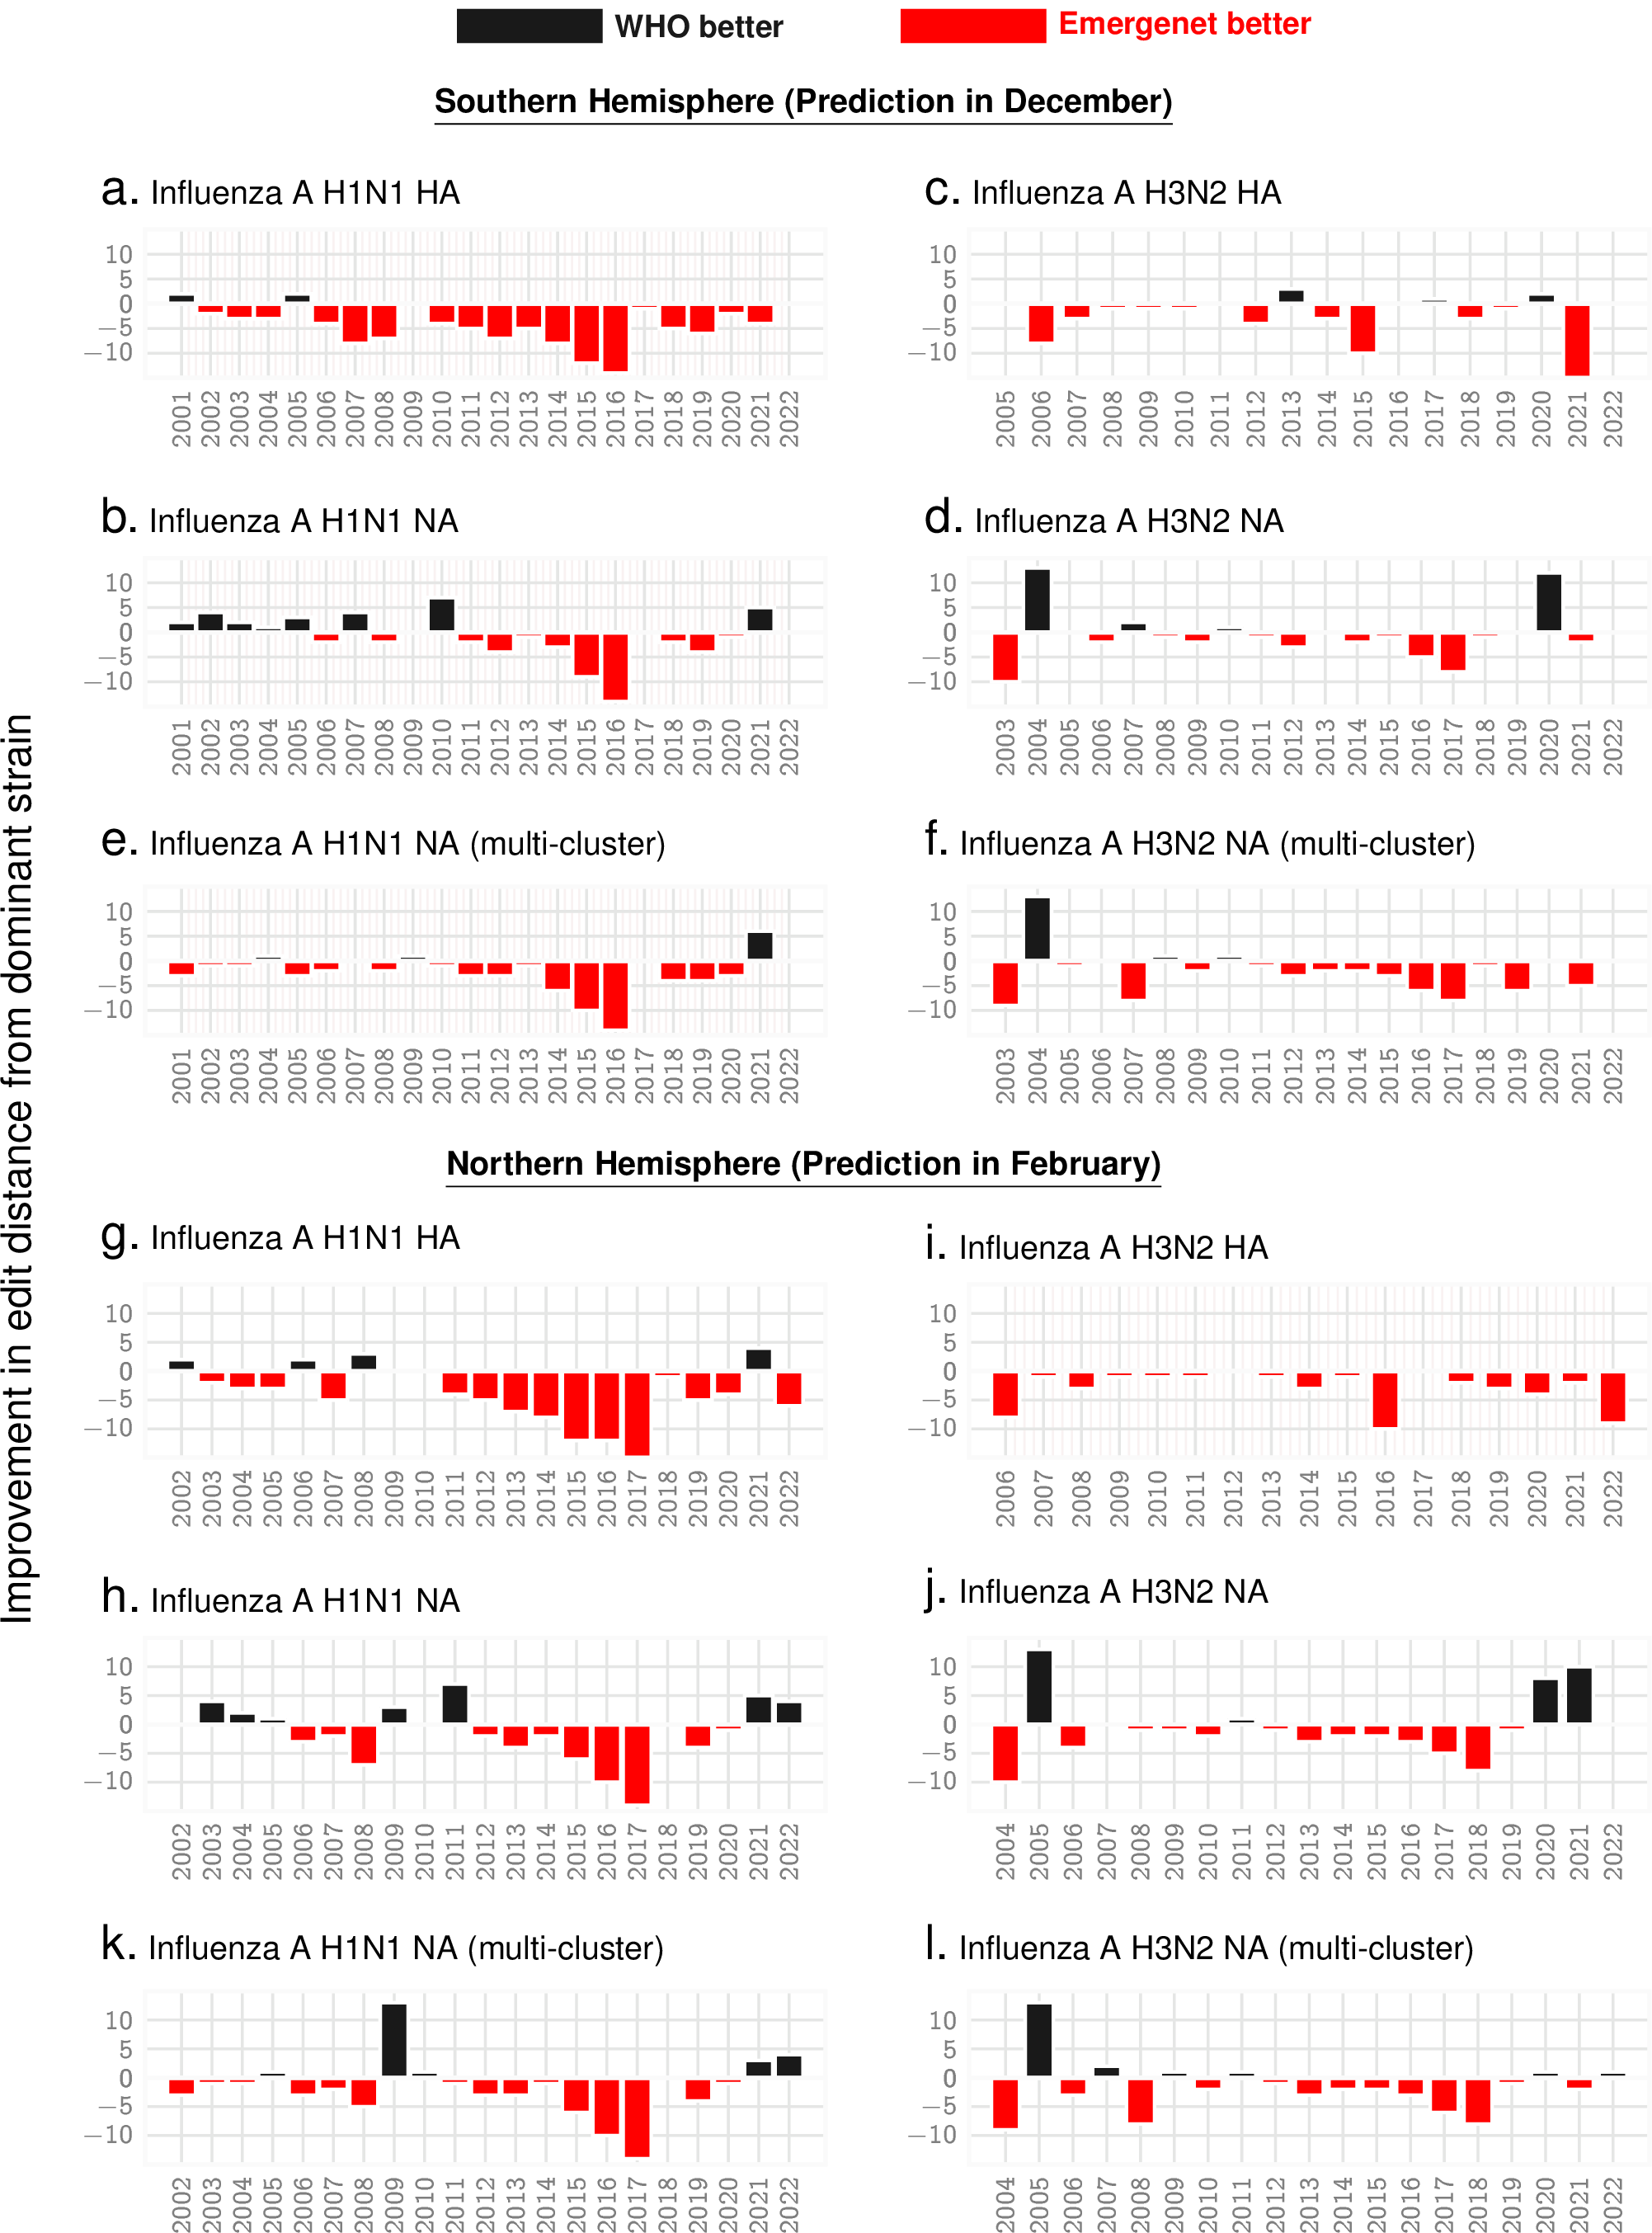
\includegraphics[width=0.975\textwidth]{Figures/seasonalpred_both.tex}
   \fi
   \captionN{\textbf{Seasonal predictions for Influenza A.} Relative out-performance of \qnet predictions against WHO recommendations for H1N1 and H3N2 sub-types for the HA and NA coding sequences over the both hemispheres. The negative bars (red) indicate the reduced edit distance between the predicted sequence and the actual dominant strain that emerged that year. Note that the recommendations for the north are given in February, while that for the south are given at the previous December, keeping in mind that the flu season in the south begins a few months early (e.g. for the 2021-2022 flu season, southern data in the table is labelled `2021' and northern is labelled `2022'). \textbf{Panels e, f, k, l} show further possible improvement in NA predictions if we return three recommendations instead of one each year.}\label{figseasonal}
\end{figure*}
\else
\refstepcounter{figure}\label{figseasonal}
\fi
%#############################################
%#############################################
%#############################################
%#############################################
\ifFIGS
\begin{figure*}[!ht]
  \tikzexternalenable
  \tikzsetnextfilename{figpred}
  \centering
 %\tikzXtrue
  \iftikzX 
   \begin{tikzpicture}[font=\sffamily\fontsize{10}{9}\selectfont]
    \def\RFILE{Figures/plotdata/fulldataframe.csv}
  \def\WDT{4.10in}
  \def\HGT{4.35in}
  \def\WDTs{1.6in}
  \def\HGTs{1.6in}
  \def\OPC{.2}
  \def\XFT{-.765in}
\def\TEXTCOLA{black!50}
\def\MCOL{DodgerBlue1!60}
\def\COLBLUE{DodgerBlue3}
\def\DCOL{black}
\def\TXTSZ{6}
\def\GGCOL{black!15}
      \def\FCOL{DarkOrange1!50}
      \def\FCOLA{DarkOrange2!50}
  \def\AXISCOL{black!15}

  \coordinate (Z) at (0,0);
    \node[] (A) at (Z) {
  \begin{tikzpicture}[anchor=center]

  \pgfplotsset{
    discard if/.style 2 args={
      x filter/.append code={
        \edef\tempa{\thisrow{#1}}
        \edef\tempb{#2}
        \ifx\tempa\tempb
        \def\pgfmathresult{inf}
        \fi
      }
    },
    discard if not/.style 2 args={
      x filter/.append code={
        \edef\tempa{\thisrow{#1}}
        \edef\tempb{#2}
        \ifx\tempa\tempb
        \else
        \def\pgfmathresult{inf}
        \fi
      }
    },
    % define the style of the `nodes near coords' that should be shown
    % above the point
    nodes near coords above style/.style={
      font=\bf\fontsize{\TXTSZ}{5}\selectfont,
      text=\TEXTCOLA,
      nodes near coords style={
        anchor=south west,yshift=.07in,
      },
    },
    % define the style of the `nodes near coords' that should be shown
    % above the point
    nodes near coords axove style/.style={
      font=\bf\fontsize{\TXTSZ}{5}\selectfont,
      text=\TEXTCOLA,
      nodes near coords style={
        anchor=south east,yshift=.02in,
      },
    },
    % define the style of the `nodes near coords' that should be shown
    % above the point
    nodes near coords belox style/.style={
      font=\bf\fontsize{\TXTSZ}{5}\selectfont,
      text=\TEXTCOLA,
      nodes near coords style={
        anchor=north west,yshift=.0in,
      },
    },
    % define the style of the `nodes near coords' that should be shown
    % above the point
    nodes near coords beloxx style/.style={
      font=\bf\fontsize{\TXTSZ}{5}\selectfont,
      text=\TEXTCOLA,
      nodes near coords style={
        anchor=north west,yshift=.02in,
      },
    },
    % define the style of the `nodes near coords' that should be shown
    % below the point
    nodes near coords below style/.style={
       font=\bf\fontsize{\TXTSZ}{5}\selectfont,
      text=\TEXTCOLA,
     nodes near coords style={
        anchor=north, yshift=-.05in, xshift=-.1in,
      },
    },
    % define the style of the `nodes near coords' that should be shown
    % below the point
    nodes near coords right style/.style={
        font=\bf\fontsize{\TXTSZ}{5}\selectfont,
      text=\TEXTCOLA,
    nodes near coords style={
        anchor=west,xshift=.02in,
      },
    },
    % define the style of the `nodes near coords' that should be shown
    % below the point
    nodes near coords left style/.style={
       font=\bf\fontsize{\TXTSZ}{5}\selectfont,
       text=\TEXTCOLA,
    nodes near coords style={
        anchor=east,
        xshift=-.02in,yshift=-.04in,
      },
    },
    % define the style of the `nodes near coords' that should be shown
    % below the point
    nodes near coords null style/.style={
         font=\bf\fontsize{\TXTSZ}{5}\selectfont,
      text=\TEXTCOLA,
   nodes near coords style={
        anchor=west,text opacity=0,
      },
    },
  }



    \begin{axis}[enlargelimits=false,scale only axis=true,
      axis line style={\AXISCOL, opacity=1,thin, rounded corners=0pt},
      grid style={thin,\GGCOL},
      grid=both,
      enlargelimits=0.01, 
      width=\WDT, 
      height=\HGT,
      scaled ticks = false,
      x tick label style={yshift=-.05in,/pgf/number format/fixed,
        /pgf/number format/1000 sep = %\thinspace % Optional if you want to replace comma as the 1000 separator 
      },yticklabel style={/pgf/number format/fixed,
        /pgf/number format/precision=2},,xticklabel style={/pgf/number format/fixed,
        /pgf/number format/precision=2},
      major tick length=0pt,
      yticklabel style={xshift=-.015in}, nodes near coords,
      point meta=explicit symbolic,
      table/meta=strain,      axis on top=false,
      ymax=7.6,      xlabel={geometric mean of HA and NA \qdist },ylabel={IRAT emergence score},xlabel style={yshift=-.1in},ylabel style={yshift=-.15in},
%axis x line=bottom,
%axis y line=left,
ymin=2.65,
ymax=7.7,
      ]



      \addplot[smooth, ultra thick,draw=white, opacity=1,mark=none,
      nodes near coords null style, ] table[col sep=comma,
      x=geometric mean of Edistances,y=pred_GM] \RFILE;

      \addplot[nodes near coords null style,forget plot,
      name path=UB,smooth, ultra thick,
      mark=none,draw=none ] table[col sep=comma,
      x=geometric mean of Edistances,y=ub_GM] \RFILE;
      
      \addplot[nodes near coords null style,
      forget plot, name path=LB,smooth,
      ultra thick, mark=none,draw=none ] table[col sep=comma,
      x=geometric mean of Edistances,y=lb_GM] \RFILE;
      
      \addplot[nodes near coords null style,
      forget plot,\FCOLA,opacity=1] fill between[of=LB and UB];
      
      
      \addplot[only marks, mark=*,
      mark options={fill=black,fill=\MCOL,draw=\DCOL,scale=1.5},
      nodes near coords below style,      
      discard if={strain}{A/Shanghai/02/2013},
      discard if={strain}{A/Indiana/08/2011},
      discard if={strain}{A/Ohio/13/2017},
      discard if={strain}{A/Hong Kong/125/2017},
      discard if={strain}{A/Sichuan/06681/2021},
      discard if={strain}{A/California/62/2018},
      discard if={strain}{A/Bangladesh/0994/2011},
      discard if={strain}{A/Anhui-Lujiang/39/2018},
      discard if={strain}{A/chicken/Tennessee/17-007431-3/2017},
      discard if={strain}{A/chicken/Tennessee/17-007147-2/2017},
      discard if={strain}{A/Yunnan/14564/2015},
      discard if={strain}{A/Astrakhan/3212/2020},
      discard if={strain}{A/canine/Illinois/12191/2015},
      discard if={strain}{A/gyrfalcon/Washington/41088/2014},
      discard if={strain}{A/turkey/Indiana/1573-2/2016},
      discard if={strain}{A/American wigeon/South Carolina/AH0195145/2021},
      discard if={strain}{A/Jiangxi-Donghu/346/2013},
      %discard if={strain}{A/swine/Shandong/1207/2016},
      discard if={strain}{A/American green-winged teal/Washington/1957050/2014},
      discard if={strain}{A/Northern pintail/Washington/40964/2014},
      discard if={strain}{A/Netherlands/219/2003} ]
      table[x=geometric mean of Edistances,
      y=IRAT Emergence Estimate,col sep=comma] \RFILE;


      \pgfplotsinvokeforeach {
        A/canine/Illinois/12191/2015,
        A/Netherlands/219/2003%
      } {
        \addplot+ [only marks,
        mark=*,
        mark options={fill=\MCOL,draw=\DCOL,scale=1.5},
        nodes near coords below style,
        forget plot,text=black,
        nodes near coords above style,
        discard if not={strain}{#1},
        ] table[x=geometric mean of Edistances,
        y=IRAT Emergence Estimate,col sep=comma]\RFILE;
      }


      \pgfplotsinvokeforeach {
        A/turkey/Indiana/1573-2/2016,
        A/American green-winged teal/Washington/1957050/2014,
        A/chicken/Tennessee/17-007147-2/2017,
        A/Northern pintail/Washington/40964/2014,
        A/American wigeon/South Carolina/AH0195145/2021,
        A/chicken/Tennessee/17-007431-3/2017,A/Astrakhan/3212/2020,
        A/Yunnan/14564/2015%
      } {
        \addplot+ [only marks,
        mark=*,mark options={fill=black,fill=\MCOL,draw=\DCOL,scale=1.5},
        forget plot,
        nodes near coords right style,
        discard if not={strain}{#1},
        ] table[x=geometric mean of Edistances,
        y=IRAT Emergence Estimate,col sep=comma]\RFILE;
      }

      \pgfplotsinvokeforeach {
       % A/swine/Shandong/1207/2016,
        A/Indiana/08/2011,
        A/Shanghai/02/2013,
        A/Hong Kong/125/2017,
        A/Sichuan/06681/2021,
        A/Bangladesh/0994/2011,
        A/Anhui-Lujiang/39/2018,
        A/California/62/2018% 
      } {
        \addplot+ [only marks,
        mark=*,mark options={fill=black,fill=\MCOL,draw=\DCOL,scale=1.50},
        forget plot,
        nodes near coords left style,
        discard if not={strain}{#1},
        ] table[x=geometric mean of Edistances,
        y=IRAT Emergence Estimate,col sep=comma]\RFILE;
      }

      \pgfplotsinvokeforeach {
        A/Ohio/13/2017,
      } {
        \addplot+ [only marks,
        mark=*,mark options={fill=black,fill=\MCOL,draw=\DCOL,scale=1.50},
        forget plot,
        nodes near coords axove style,
        discard if not={strain}{#1},
        ] table[x=geometric mean of Edistances,
        y=IRAT Emergence Estimate,col sep=comma]\RFILE;
      }

     \pgfplotsinvokeforeach {
 A/gyrfalcon/Washington/41088/2014,
      } {
        \addplot+ [only marks,
        mark=*,mark options={fill=black,fill=\MCOL,draw=\DCOL,scale=1.50},
        forget plot,
        nodes near coords belox style,
        discard if not={strain}{#1},
        ] table[x=geometric mean of Edistances,
        y=IRAT Emergence Estimate,col sep=comma]\RFILE;
      }
     \pgfplotsinvokeforeach {A/Jiangxi-Donghu/346/2013,
      } {
        \addplot+ [only marks,
        mark=*,mark options={fill=black,fill=\MCOL,draw=\DCOL,scale=1.50},
        forget plot,
        nodes near coords beloxx style,
        discard if not={strain}{#1},
        ] table[x=geometric mean of Edistances,
        y=IRAT Emergence Estimate,col sep=comma]\RFILE;
      }

      \node [anchor=center,font=\bf\sffamily\fontsize{6}{6}\selectfont] at (axis cs:-0.23,3) {H7N9};
      \node [anchor=center,font=\bf\sffamily\fontsize{6}{6}\selectfont] at (axis cs:-0.16,3.265) {H7N9};
  \node [anchor=center,font=\bf\sffamily\fontsize{6}{6}\selectfont] at (axis cs:-0.31,5.2) {H5N6};
  \node [anchor=center,font=\bf\sffamily\fontsize{6}{6}\selectfont] at (axis cs:-0.315,4.45) {H7N7};
 \node [anchor=center,font=\bf\sffamily\fontsize{6}{6}\selectfont] at (axis cs:-0.296,4.25) {H5N1};
  \node [anchor=center,font=\bf\sffamily\fontsize{6}{6}\selectfont] at (axis cs:-0.296,3.27) {H7N8};
   \node [anchor=center,font=\bf\sffamily\fontsize{6}{6}\selectfont] at (axis cs:-0.31,3.6) {H5N1};
  \node [anchor=center,font=\bf\sffamily\fontsize{6}{6}\selectfont] at (axis cs:-0.26,3.8) {H5N2};
 \node [anchor=center,font=\bf\sffamily\fontsize{6}{6}\selectfont] at (axis cs:-0.25,4.6) {H5N8};
   \node [anchor=center,font=\bf\sffamily\fontsize{6}{6}\selectfont] at (axis cs:-0.245,4.2) {H5N8};
      \node [anchor=center,font=\bf\sffamily\fontsize{6}{6}\selectfont] at (axis cs:-0.225,4.3) {H10N8};
      \node [anchor=center,font=\bf\sffamily\fontsize{6}{6}\selectfont] at (axis cs:-0.19,5.8) {H9N2};
      \node [anchor=center,font=\bf\sffamily\fontsize{6}{6}\selectfont] at (axis cs:-0.15,5.42) {H5N6};
      \node [anchor=center,font=\bf\sffamily\fontsize{6}{6}\selectfont] at (axis cs:-0.08,3.7) {H3N2};
      \node [anchor=center,font=\bf\sffamily\fontsize{6}{6}\selectfont] at (axis cs:-0.067,5.8) {H1N2};
      \node [anchor=center,font=\bf\sffamily\fontsize{6}{6}\selectfont] at (axis cs:-0.055,6.2) {H9N2};
      \node [anchor=center,font=\bf\sffamily\fontsize{6}{6}\selectfont] at (axis cs:-0.06,7.5) {H1N1};
      \node [anchor=center,font=\bf\sffamily\fontsize{6}{6}\selectfont] at (axis cs:-0.06,5.2) {H5N1};
      \node [anchor=center,font=\bf\sffamily\fontsize{6}{6}\selectfont] at (axis cs:-0.0375,6.6) {H3N2};
      \node [anchor=center,font=\bf\sffamily\fontsize{6}{6}\selectfont] at (axis cs:-0.08,6.55) {H7N9};
      \node [anchor=center,font=\bf\sffamily\fontsize{6}{6}\selectfont] at (axis cs:-0.02,6.25) {H7N9};
      \node [anchor=center,font=\bf\sffamily\fontsize{6}{6}\selectfont] at (axis cs:-0.02,5.85) {H3N2};


            \node [text=\COLBLUE,anchor=north west,fill=white,align=left,font=\bf\sffamily\fontsize{8}{9}\selectfont] (LLEQ1) at (axis cs:-.25,6.5) {$R = 0.703$\\p-value\\$0.00026$};


    \end{axis}
  \end{tikzpicture}};
\node[anchor=north west] (B) at ([xshift=\XFT]A.north east) {
      \def\RFILE{Figures/plotdata/fulldataframe_sortE.csv}

  \begin{tikzpicture}[anchor=center]
\begin{axis}[enlargelimits=false,scale only axis=true,
      axis line style={\AXISCOL, opacity=1,thin, rounded corners=0pt},
      grid style={thin,\GGCOL},
      grid=both,
      enlargelimits=0.015, 
      width=\WDTs, 
      height=\HGTs,
      scaled ticks = false,
      x tick label style={yshift=-.05in,/pgf/number format/fixed,
        /pgf/number format/1000 sep = %\thinspace % Optional if you want to replace comma as the 1000 separator 
      },yticklabel style={/pgf/number format/fixed,
        /pgf/number format/precision=2},,xticklabel style={/pgf/number format/fixed,
        /pgf/number format/precision=2},
      major tick length=0pt,
      yticklabel style={xshift=-.015in}, %nodes near coords,
      %point meta=explicit symbolic,
      %table/meta=strain,
      axis on top=false,
      ymax=7.6,
      xmin=3.25,xmax=6.8,      xlabel={predicted emergence score},
      ylabel={IRAT emergence score},,xlabel style={yshift=-.05in,xshift=0in},ylabel style={yshift=-.225in},
      ]

        \addplot[smooth, only marks, mark=*, mark options={fill=white,scale=.8},, opacity=1,mark=none, ] table[col sep=comma,
      y=IRAT Emergence Estimate,x=Emergenet emergence estimate] \RFILE;

      \addplot[smooth, ultra thick,draw=white, opacity=1,mark=none, ] table[col sep=comma,
      y=pred_E,x=Emergenet emergence estimate] \RFILE;

      \addplot[forget plot,
      name path=UB,smooth, ultra thick,
      mark=none,draw=none ] table[col sep=comma,
      y=ub_E,x=Emergenet emergence estimate] \RFILE;
      
      \addplot[forget plot, name path=LB,smooth,
      ultra thick, mark=none,draw=none ] table[col sep=comma,
      y=lb_E,x=Emergenet emergence estimate] \RFILE;
      
      \addplot[forget plot,\FCOL,opacity=1] fill between[of=LB and UB];

      \node [text=\COLBLUE,anchor=north west,fill=white] (LLEQ1) at (axis cs:3.3,7) {OLS fit: $y=x$};

        \node [text=\COLBLUE,anchor=north west,fill=white,align=left,font=\bf\sffamily\fontsize{8}{9}\selectfont] (LLEQ1) at (axis cs:5,4) {$R = 0.81$\\p-value\\$4.7\times 10^{-6}$};

\end{axis}
  \end{tikzpicture}
  };


\node[anchor=south west] (C) at ([xshift=\XFT]A.south east) {
      \def\RFILE{Figures/plotdata/fulldataframe_sortI.csv}

  \begin{tikzpicture}[anchor=center]
\begin{axis}[enlargelimits=false,scale only axis=true,
      axis line style={\AXISCOL, opacity=1,thin, rounded corners=0pt},
      grid style={thin,\GGCOL},
      grid=both,
      enlargelimits=0.015, 
      width=\WDTs, 
      height=\HGTs,
      scaled ticks = false,
      x tick label style={yshift=-.05in,/pgf/number format/fixed,
        /pgf/number format/1000 sep = %\thinspace % Optional if you want to replace comma as the 1000 separator 
      },yticklabel style={/pgf/number format/fixed,
        /pgf/number format/precision=2},,xticklabel style={/pgf/number format/fixed,
        /pgf/number format/precision=2},
      major tick length=0pt,
      yticklabel style={xshift=-.015in}, %nodes near coords,
      %point meta=explicit symbolic,
      %table/meta=strain,
      axis on top=false,
      ymax=7.6,      xmin=3.75,xmax=6.8,
      xlabel={predicted impact score},
      ylabel={IRAT impact score},,xlabel style={yshift=-.05in,xshift=0in},ylabel style={yshift=-.225in},
      ]

      
      \addplot[smooth, only marks, mark=*, mark options={fill=white,scale=.8},, opacity=1,mark=none, ] table[col sep=comma,
      y=IRAT Impact Estimate,x=Emergenet impact estimate] \RFILE;

      \addplot[smooth, ultra thick,draw=white, opacity=1,mark=none, ] table[col sep=comma,
      y=pred_I,x=Emergenet impact estimate] \RFILE;

      \addplot[forget plot,
      name path=UB,smooth, ultra thick,
      mark=none,draw=none ] table[col sep=comma,
      y=ub_I,x=Emergenet impact estimate] \RFILE;
      
      \addplot[forget plot, name path=LB,smooth,
      ultra thick, mark=none,draw=none ] table[col sep=comma,
      y=lb_I,x=Emergenet impact estimate] \RFILE;
      
      \addplot[forget plot,\FCOL,opacity=1] fill between[of=LB and UB];


      \node [text=\COLBLUE,anchor=north west,fill=white] (LLEQ1) at (axis cs:3.7,7) {OLS fit: $y=x$};
        \node [text=\COLBLUE,anchor=north west,fill=white,align=left,font=\bf\sffamily\fontsize{8}{9}\selectfont] (LLEQ1) at (axis cs:5.25,4.5) {$R = 0.77$\\p-value\\$3.3\times 10^{-5}$};
\end{axis}
  \end{tikzpicture}
  };


  \node[anchor=north west] (W) at ([yshift=-.4in]A.south west) {
    \begin{tikzpicture}[font=\bf\sffamily\fontsize{8}{8}\selectfont]
 \begin{scope}
 \clip (-3.4in,1.25in) rectangle (3.35in,-1in);
\node[anchor=center] (A11) at (0,0) {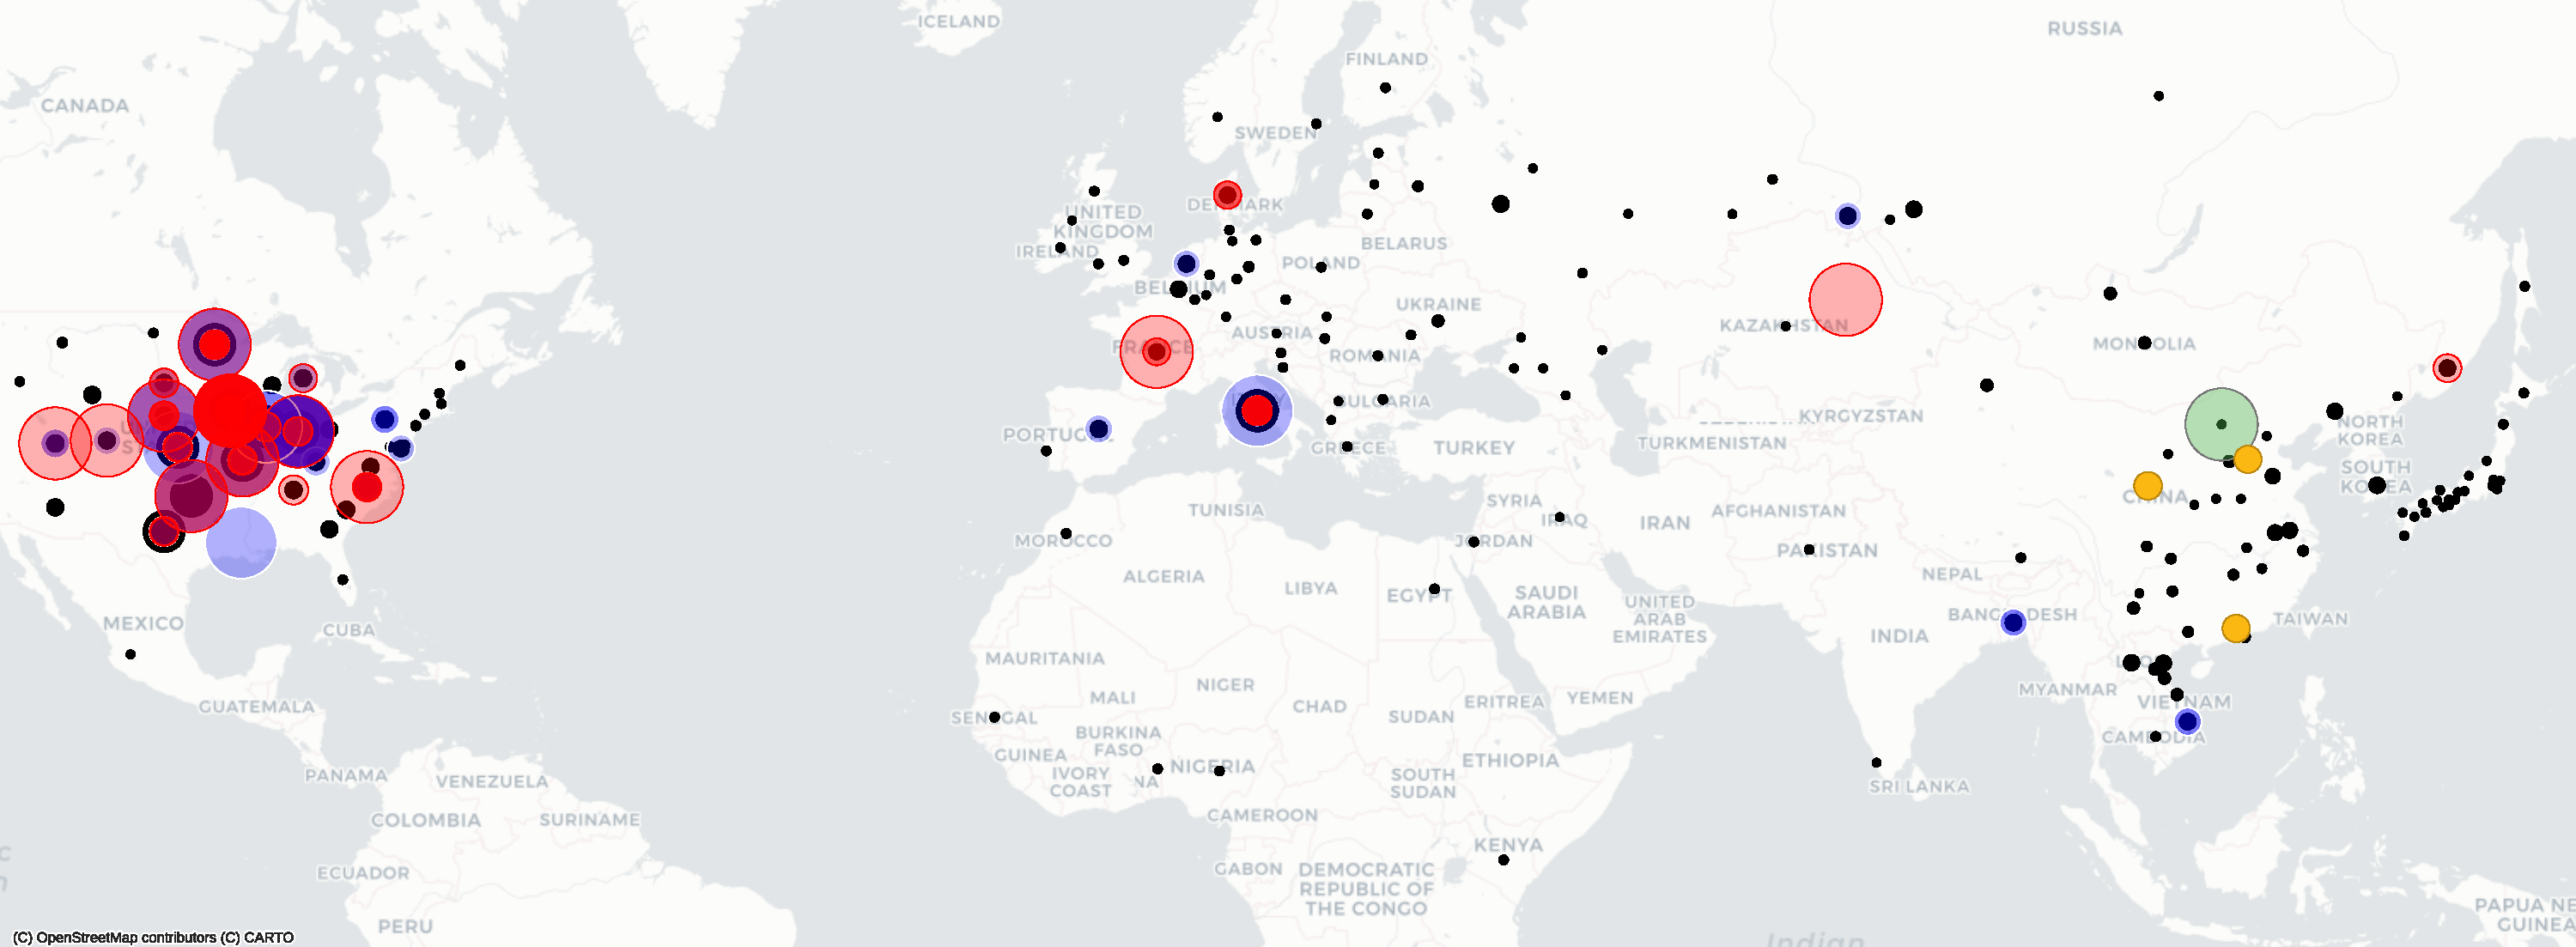
\includegraphics[width=\textwidth]{Figures/bionorad}};
\end{scope}

%7.5 7.2 6.8 <6
\def\TEXTCOLA{black!60}

\node[circle,fill=white,inner sep=1pt,text width=.195in,draw=\TEXTCOLA,label={[text=gray,align=center,font=\bf\sffamily\fontsize{7}{8}\selectfont]90:Geometric mean of\\predicted impact and emergence  scores}] (C1) at ([xshift=-1.65in,yshift=.9in]A11.center) {};
\node [anchor=west,align=left,text=\TEXTCOLA,] (LL1) at ([xshift=.1in]C1.center) {$7.5$};
\node[circle,fill=white,text width=.175in,draw=\TEXTCOLA,inner sep=1pt,,anchor=north,text=\TEXTCOLA] (C1) at ([yshift=-.1in]C1.south) {};
\node[circle,fill=white,text width=.11in,draw=\TEXTCOLA,inner sep=1pt,,anchor=north,text=\TEXTCOLA] (C1) at ([yshift=-.1in]C1.south) {};
\node[circle,fill=white,text width=.075in,inner sep=1pt,draw=\TEXTCOLA,,anchor=north,text=\TEXTCOLA] (C1) at ([yshift=-.1in]C1.south) {};
\node[circle,fill=white,inner sep=1pt,text width=.005in,draw=\TEXTCOLA,,anchor=north,text=\TEXTCOLA] (C1) at ([yshift=-.12in]C1.south) {};
\node [anchor=north,align=left,text=\TEXTCOLA] (LL1) at ([yshift=-.15in]LL1.south) {$7.2$};
\node [anchor=north,align=left,text=\TEXTCOLA] (LL1) at ([yshift=-.11in]LL1.south) {$6.8$};
\node [anchor=north,align=left,text=\TEXTCOLA] (LL1) at ([yshift=-0.06in]LL1.south) {$6.7$};
\node [anchor=north,align=left,text=\TEXTCOLA] (LL1) at ([yshift=-0.03in]LL1.south) {$6.0$};

\node[font=\sffamily\fontsize{6}{6}\selectfont,align=center,fill=Red1!60,text width=.25in,anchor=north,xshift=-.05in,yshift=-.351in,label={[font=\bf\sffamily\fontsize{7}{8}\selectfont,xshift=.1in,text=gray]90:subtypes of high-risk strains}] (X1) at (C1.south) {H1N1};
\node[font=\sffamily\fontsize{6}{6}\selectfont,align=center,text=white,fill=Blue1!60,text width=.25in,anchor=north,xshift=0in,yshift=-.051in] (X2) at (X1.south) {H3N2};
\node[font=\sffamily\fontsize{6}{6}\selectfont,align=center,text=white,fill=Yellow3!70!black,text width=.25in,anchor=west,xshift=0.02in,yshift=0in] (X1) at (X1.east) {H5N2};
\node[font=\sffamily\fontsize{6}{6}\selectfont,align=center,fill=Green4!50,text width=.25in,anchor=north,xshift=0in,yshift=-.051in] (X1) at (X1.south) {H7N9};


\node [] (LD1) at ([yshift=.5in,xshift=1in]A11.center) {};
\draw [] (LD1)node [right,above,align=center,font=\bf\sffamily\fontsize{5}{5}\selectfont] {A/chicken/Bulgaria/221\_20VIR1725-1/2020\\(emergence: 6.4, impact: 8.8)}  -- ++(-.4in,0in) -- ++(-.2in,-.19in) ;




\node [text=Red1] (LD2) at ([yshift=.47in,xshift=-.25in]A11.east) {};
\draw [] (LD2) node [xshift=-.2in,right,above,align=right,font=\bf\sffamily\fontsize{5}{5}\selectfont,xshift=-.25in] {A/Chicken/Hebei/1011/2021\\(emergence: 6.7, impact: 7.7)}  -- ++(-.4in,0in) -- ++(-.2in,-.2in) ;


\node [text=Red1] (LD3) at ([yshift=.85in,xshift=-2.05in]A11.east) {};
\draw [] (LD3) node [right,above,align=center,font=\bf\sffamily\fontsize{5}{5}\selectfont,xshift=-.25in] {A/Camel/Inner\_Mongolia/XL/2020\\(emergence: 6.8, impact: 6.7)}  -- ++(.4in,0in) -- ++(.6in,-.6in) ;



\node [text=Red1] (LD4) at ([yshift=-.25in,xshift=.75in]A11.west) {};
\draw [] (LD4) node [right,above,xshift=.65in,align=center,font=\bf\sffamily\fontsize{5}{5}\selectfont,xshift=-.25in] {A/swine/Missouri/A02524711/2020\\(emergence: 6.8, impact: 6.7)}  -- ++(-.4in,0in) -- ++(.3in,.3in) ;

\end{tikzpicture}
    };

  
\node[anchor=south west] (LA) at (A.north west) {{\Large a.} \bf Predicted emergence risk vs published IRAT scores};
\node[anchor=south west,align=left] (LB) at ([xshift=0in]B.north west) {{\Large b.} \bf Estimating emergence};
\node[anchor=south west] (LC) at ([xshift=.1in]C.north west) {{\Large c.} \bf Estimating  impact};
\node[anchor=south west] (LW) at ([xshift=.1in]W.north west) {{\Large d.} \bf Global prediction of IRAT scored for all \infl sequences collected since 2020};


\end{tikzpicture}
    
   \else 
   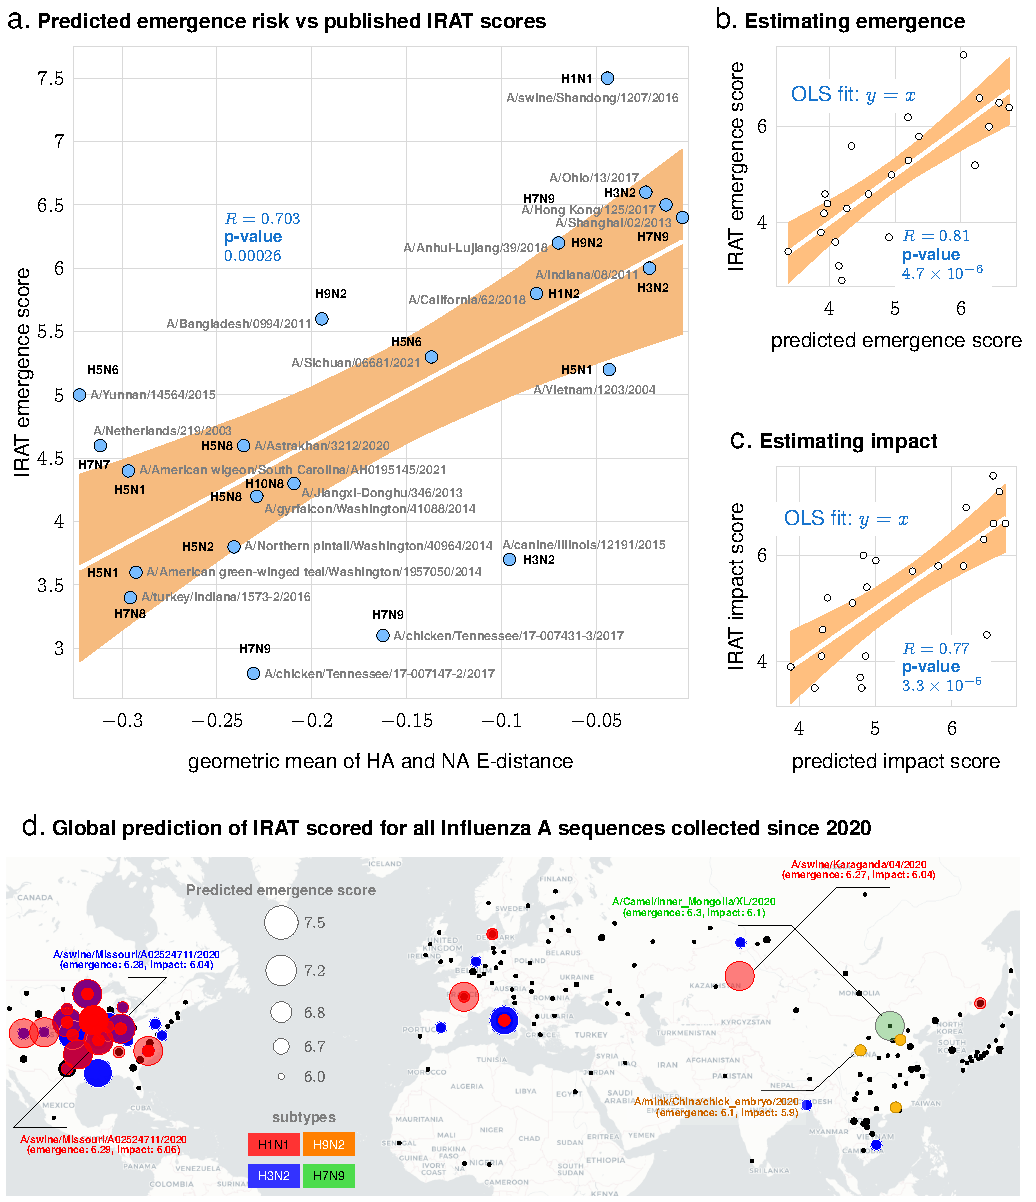
\includegraphics[width=\textwidth]{Figures/External/figpred}
   \fi
   \vspace{-20pt}
   
  \captionN{\textbf{\enet based estimation of IRAT score}. Panel a. There is an approximate linear relationship between average q-distance from human circulating strains (geometric mean of the \qdist for  HA and NA sequences) and the published IRAT emergence score calculated by CDC. Panel b. Estimation of the IRAT emergence score via fitting a  GLM model to  the \qdist{es} estimated from the \enet.  Panel c. Estimation of IRAT impact scores via fitting a separate GLM model to the the \qdist{es} estimated from the \enet. Panel d. Identifying risky \infl strains amongst those collected between 2020 and 2022 April, via  our IRAT emergence score estimation framework.
  }\label{figirat}
\end{figure*}
\else
\refstepcounter{figure}\label{figirat}
\fi
%#############################################
%#############################################
\ifFIGS

\begin{figure}[!ht]\centering
\centering
 \tikzexternalenable
  \tikzsetnextfilename{figphylo}
  \centering
%\tikzXtrue
  \iftikzX 
   \begin{tikzpicture}[font=\bf\sffamily\fontsize{9}{9}\selectfont]

  
\node[] (A) at (0,0) {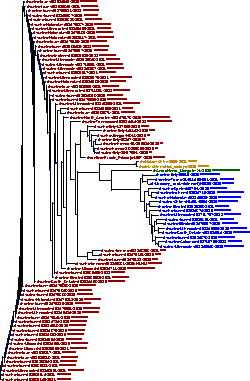
\includegraphics[width=.9\textwidth]{Figures/riskyphylo6_collapsed_19}};

\draw[line width=10pt] ([yshift=.5in,xshift=1.28in]A.south) node (DA) [left,below]{6.0} -- ++(.7in,0) node (DB) [right,below] {6.3};
\node[anchor=south] (L1)  at ([yshift=.15in]$(DA.north)!.5!(DB.north)$) {estimated IRAT emergence score};

\coordinate (C1) at ([xshift=-.125in,yshift=1in]L1.north) ;

\node[align=center,fill=Red4!80!black,text=white,,text width=.35in,anchor=north,xshift=-0.05in,yshift=-.3in,label={[font=\bf\sffamily\fontsize{9}{9}\selectfont,
  xshift=.2in,text=gray]90:subtypes of risky strains}] (X1) at (C1.south) {H1N1};
\node[align=center,text=white,fill=Blue1!80,text width=.35in,anchor=north,xshift=0in,yshift=-.051in] (X2) at (X1.south) {H3N2};
\node[align=center,text=white,fill=DarkOrange2,text width=.35in,anchor=west,xshift=0.02in,yshift=0in] (X1) at (X1.east) {H9N2};
\node[text=white,align=center,fill=Green4,text width=.35in,anchor=north,xshift=0in,yshift=-.051in] (X1) at (X1.south) {H7N9};

\def\FCOLX{Red1}


\node[shape=isosceles triangle,fill=\FCOLX,rotate=90 ] (h1n1strain) at ([xshift=-.95in,yshift=1.85in]L1.north) {};

\node[anchor=west] at ([xshift=.1in,yshift=-.1in]h1n1strain.east) {
\includegraphics[width=.5in]{Figures/animalicons/pig}};

\node[shape=isosceles triangle,fill=\FCOLX,rotate=-90 ] (h7n9strain) at ([xshift=.85in,yshift=4.65in]L1.north) {};
\node[anchor=west] at ([xshift=-.2in,yshift=0.45in]h7n9strain.east) {
\includegraphics[width=.5in]{Figures/animalicons/camel}};

\node[shape=isosceles triangle,fill=\FCOLX,rotate=-90 ] (h3n2strain) at ([xshift=1.22in,yshift=4.1in]L1.north) {};
\node[anchor=west] at ([xshift=-.25in,yshift=0.35in]h3n2strain.east) {
\includegraphics[width=.4in]{Figures/animalicons/pig}};

\node[shape=isosceles triangle,fill=\FCOLX,rotate=-90 ] (h9n2strain) at ([xshift=.3in,yshift=4.9in]L1.north) {};
\node[anchor=west] (mink) at ([xshift=-.25in,yshift=0.4in]h9n2strain.east) {
\includegraphics[width=.6in]{Figures/animalicons/mink}};

\node[anchor=west,opacity=.5] (cc) at ([xshift=-3in,yshift=-1in]h9n2strain.east) {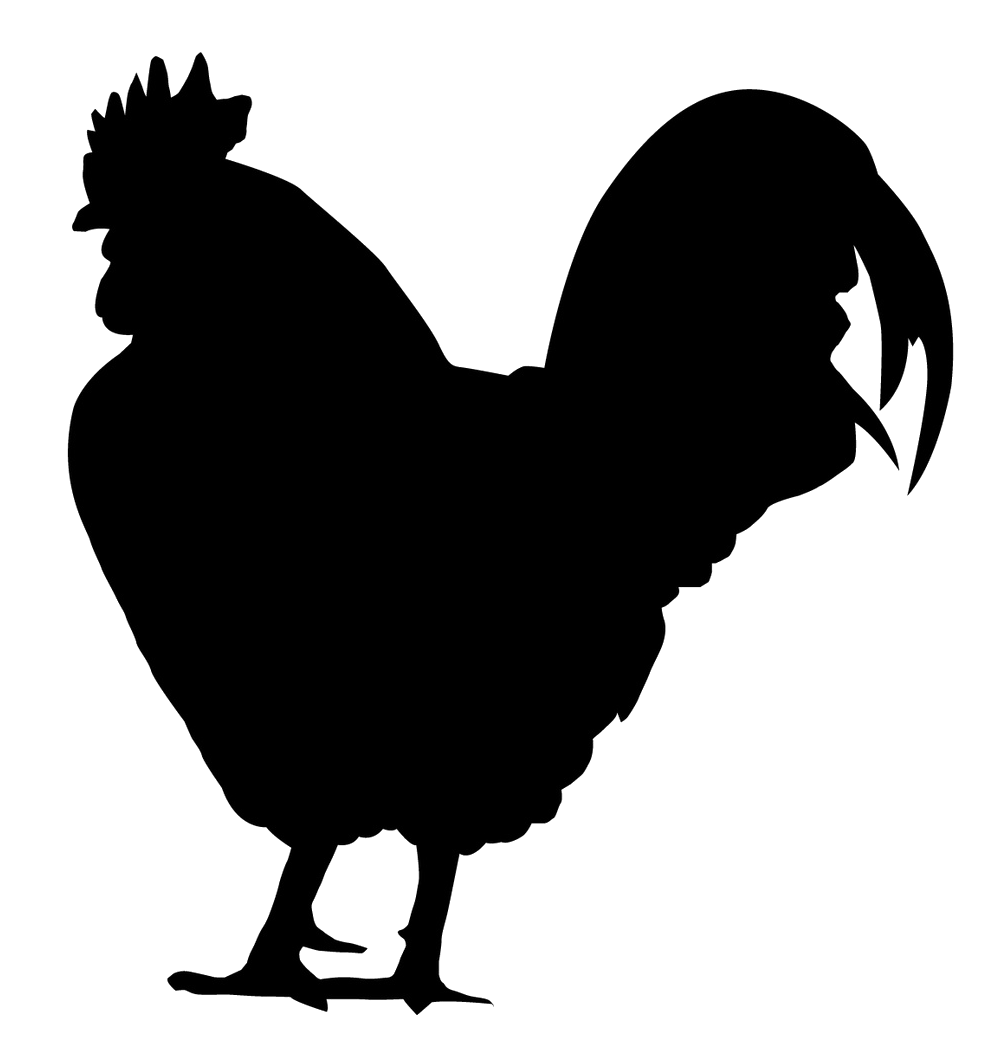
\includegraphics[width=.5in]{Figures/animalicons/chicken}};
\node[anchor=west,opacity=.5] (dd) at ([xshift=-2.5in,yshift=-1.45in]h9n2strain.east) {
\includegraphics[width=.6in]{Figures/animalicons/dog}};
\node[anchor=west,opacity=.5] (dc) at ([xshift=-2in,yshift=-1.85in]h9n2strain.east) {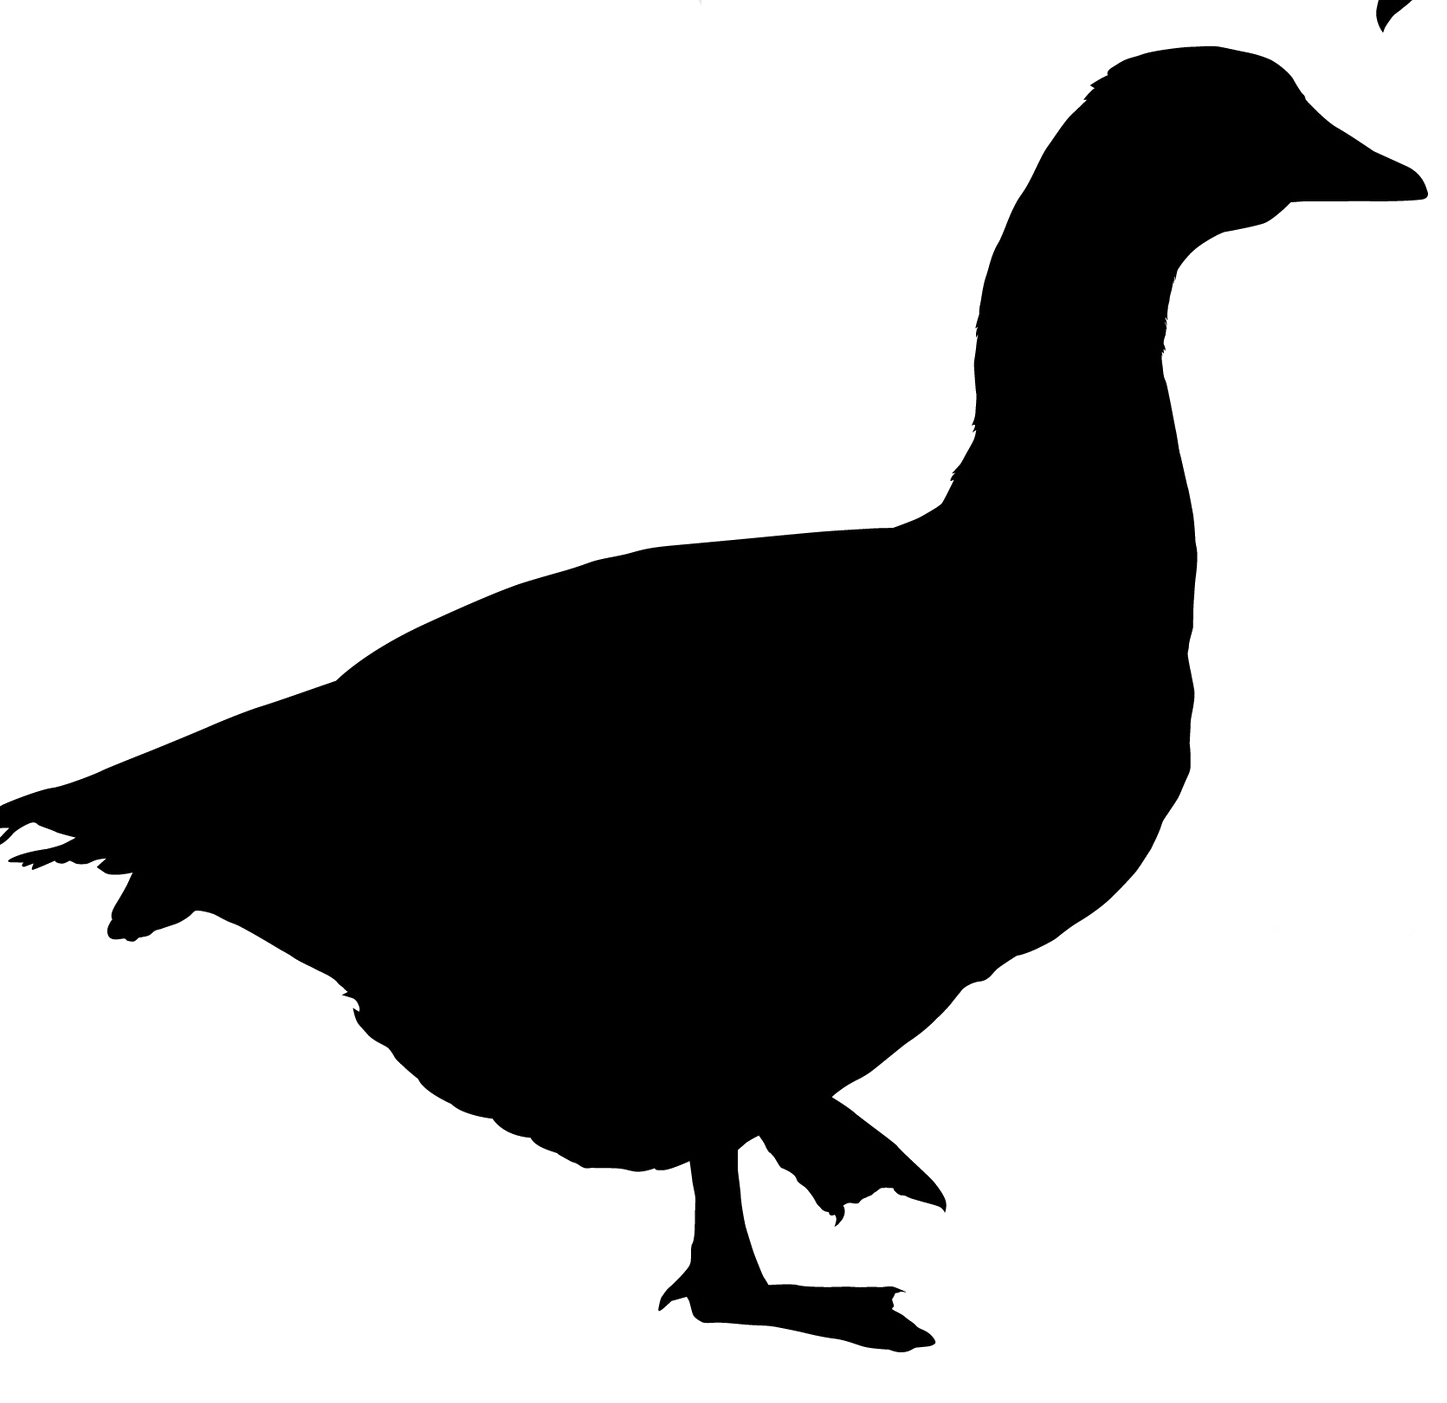
\includegraphics[width=.5in]{Figures/animalicons/duck2}};

\node[anchor=south,opacity=.4] (pig2) at ([xshift=-2.2in,yshift=-5.5in]mink.north) {
\includegraphics[width=.8in]{Figures/animalicons/pig}};

\node[anchor=south,opacity=.4] (pig3) at ([xshift=-1in,yshift=1in]mink.north) {
\includegraphics[width=.8in]{Figures/animalicons/pig}};


\draw [ultra thick,dashed,opacity=.3] (cc) -- ++(1.1in,.75in);
\draw [ultra thick,dashed,opacity=.3] (dd) -- ++(.96in,.9in);
\draw [ultra thick,dashed,opacity=.3] (dc) -- ++(.6in,1.1in);
% \draw [ultra thick,dashed,opacity=.3] (pig3) -- ++(-.8in,-1.5in);
% \draw [ultra thick,dashed,opacity=.3] (pig3) -- ++(-1.6in,0in);
% \draw [ultra thick,dashed,opacity=.3] (pig3) -- ++(-1.6in,1.5in);
% \draw [ultra thick,dashed,opacity=.3] (pig2) -- ++(-.8in,-1.5in);
% \draw [ultra thick,dashed,opacity=.3] (pig2) -- ++(-1.6in,0in);
% \draw [ultra thick,dashed,opacity=.3] (pig2) -- ++(-1.6in,1.5in);

% \coordinate (CC) at ([xshift=1.5in]h1n1strain);
% \draw[opacity=.15] (h1n1strain) -- (CC);
% \draw[opacity=.15] (h3n2strain) -- (CC);
% \draw[opacity=.15] (h7n9strain) -- (CC);
% \draw[opacity=.15] (h9n2strain) -- (CC);

\end{tikzpicture}  
   \else 
   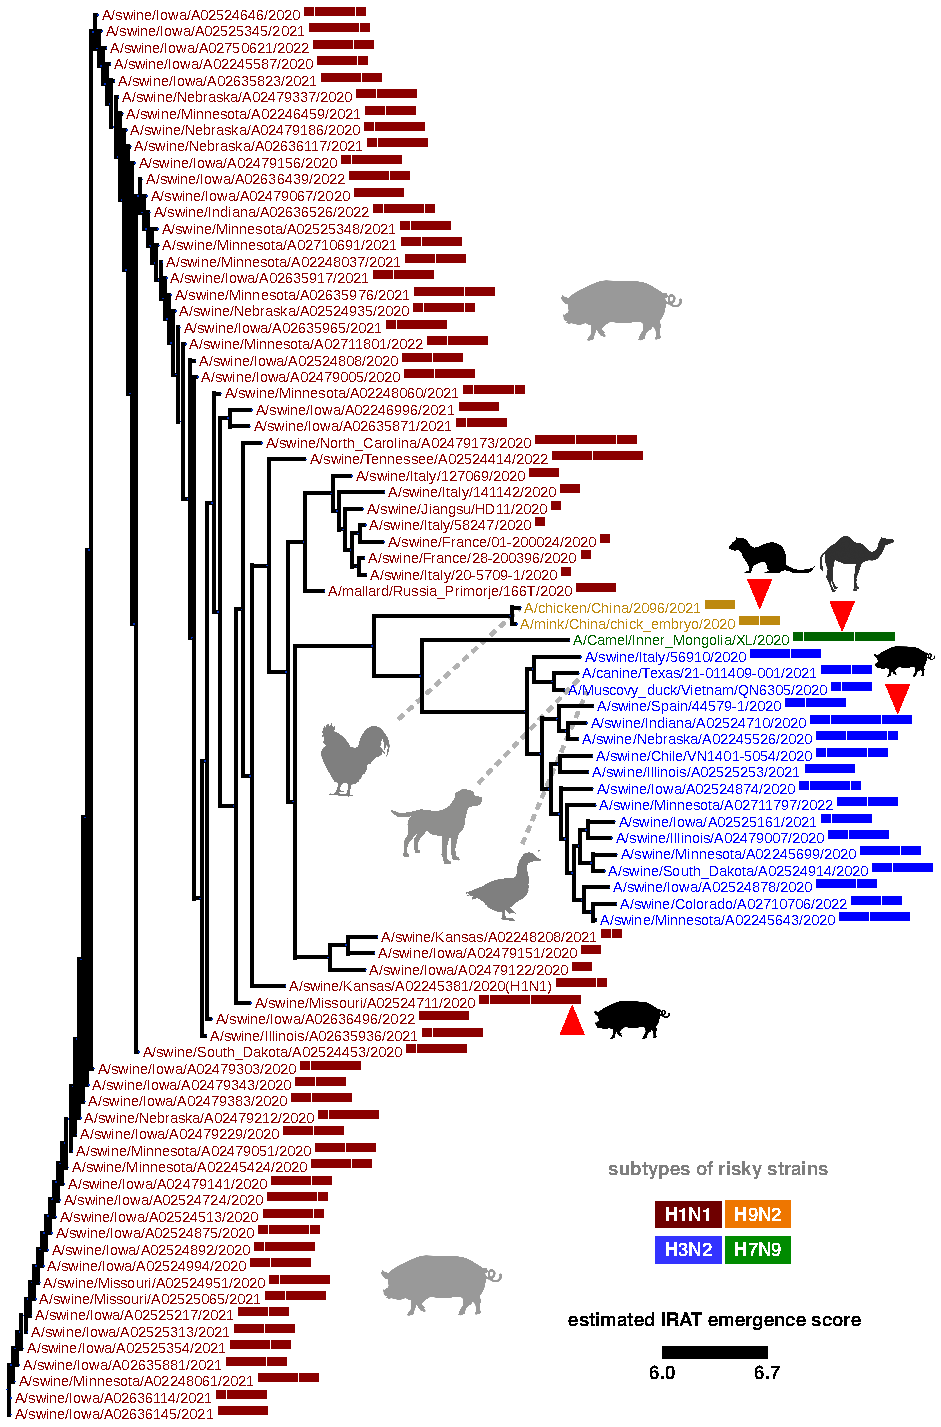
\includegraphics[width=.9\textwidth]{Figures/External/figphylo}
   \fi
   \vspace{-10pt}

\captionN{Standard phylogenetic tree constructed with edit distances,  with all  \infl strains collected between 2020 and 2022 April, with estimated IRAT emergence risk $> 6.0$, and collapsing leaves which differ by less than 15 edits in the HA, leaving the most risky strains in the leaves. The most risky strains are marted with a red arrowhead, which comes from diverse animal hosts, and geographic regions. }\label{figphylo}
\end{figure}
\else
\refstepcounter{table}\label{figphylo}
\fi
% #############################################
%#############################################
\ifFIGS

\begin{table}[!ht]\centering
\captionN{Influenza A Strains Evaluated by IRAT and Corresponding \qnet Computed Risk Scores}\label{irattab}

\sffamily\fontsize{7}{8}\selectfont

\begin{tabular}{L{1.25in}|L{.35in}|L{.3in}|L{.3in}|L{.3in}|L{.35in}|L{.35in}|L{.35in}|L{.35in}|L{.32in}|L{.3in}|L{.3in}}\hline
Influenza Virus & Subype & IRAT Date &IRAT Emergence Score &IRAT Impact Score &HA Sample &NA Sample &HA \erisk & NA \erisk &Geom. Mean&\qnet Emergence Score&\qnet Impact Score \\\hline
 A/swine/Shandong/1207/2016 &H1N1& Jul  2020 &7.5&6.9&1000&1000&-0.0941&-0.0205&0.0440&6.0&6.2\\\hline
 A/Ohio/13/2017 &H3N2& Jul  2019 &6.6&5.8&1000&1000&-0.0184&-0.0306&0.0238&6.3&6.2\\\hline
 A/Hong  Kong/125/2017 &H7N9& May  2017 &6.5&7.5&437&437&-0.0296&-0.0058&0.0131&6.6&6.5\\\hline
 A/Shanghai/02/2013 &H7N9& Apr  2016 &6.4&7.2&178&178&-0.0055&-0.0036&0.0044&6.7&6.6\\\hline
 A/Anhui-Lujiang/39/2018 &H9N2& Jul  2019 &6.2&5.9&31&30&-0.0290&-0.1681&0.0698&5.2&5.0\\\hline
 A/Indiana/08/2011 &H3N2& Dec  2012 &6.0&4.5&1000&1000&-0.0523&-0.0091&0.0218&6.4&6.5\\\hline
 A/California/62/2018 &H1N2& Jul  2019 &5.8&5.7&55&55&-0.1089&-0.0610&0.0815&5.4&5.5\\\hline
 A/Bangladesh/0994/2011$^{\star\star\star}$ &H9N2& Feb  2014 &5.6&5.4&&&-0.2078&-0.1823&0.1947&4.3&4.9\\\hline
 A/Sichuan/06681/2021 &H5N6& Oct  2021 &5.3&6.3&45&45&-0.3616&-0.0518&0.1369&5.2&6.4\\\hline
 A/Vietnam/1203/2004 &H5N1& Nov  2011 &5.2&6.6&258&246&-0.1673&-0.0111&0.0430&6.2&6.7\\\hline
 A/Yunnan/14564/2015$^{\star\star}$ &H5N6& Apr  2016 &5.0&6.6&344&331&-0.3482&-0.2987&0.3225&4.9&6.5\\\hline
 A/Astrakhan/3212/2020$^{\star\star}$ &H5N8& Mar  2021 &4.6&5.2&381&365&-0.1603&-0.3472&0.2359&3.9&4.4\\\hline
 A/Netherlands/219/2003 &H7N7& Jun  2012 &4.6&5.8&46&46&-0.2757&-0.3521&0.3115&4.6&5.8\\\hline
 A/American  wigeon/South  Carolina/AH0195145/2021 &H5N1& Mar  2022 &4.4&5.1&335&323&-0.1722&-0.5114&0.2967&4.0&4.7\\\hline
 A/Jiangxi-Donghu/346/2013$^{\star\star\star}$ &H10N8& Feb  2014 &4.3&6.0&&&-0.2088&-0.2101&0.2094&4.3&4.8\\\hline
 A/gyrfalcon/Washington/ 41088/2014$^{\star\star}$ &H5N8& Mar  2015 &4.2&4.6&341&328&-0.1532&-0.3424&0.2290&3.9&4.3\\\hline
 A/Northern  pintail/ Washington/40964/2014$^{\star\star}$ &H5N2& Mar  2015 &3.8&4.1&341&328&-0.1529&-0.3799&0.2410&3.9&4.3\\\hline
 A/canine/Illinois/12191/2015 &H3N2& Jun  2016 &3.7&3.7&1000&1000&-0.0607&-0.1509&0.0957&4.9&4.8\\\hline
 A/American  green-winged  teal /Washington/1957050/2014 &H5N1& Mar 2015 &3.6&4.1&326&314&-0.1911&-0.4482&0.2927&4.1&4.9\\\hline
 A/turkey/Indiana/1573-2/2016$^{\star\star}$ &H7N8& Jul  2017 &3.4&3.9&495&494&-0.1130&-0.7738&0.2957&3.4&3.9\\\hline
 A/chicken/Tennessee/17-007431-3/2017 &H7N9& Oct  2017 &3.1&3.5&496&495&-0.1027&-0.2569&0.1624&4.1&4.2\\\hline
 A/chicken/Tennessee/17-007147-2/2017 &H7N9& Oct  2017 &2.8&3.5&496&495&-0.2095&-0.2541&0.2307&4.2&4.8\\\hline
% A/duck/New  York/1996 $^\star$&H1N1& Nov  2011 &2.3&2.4&1000&1000&-1&-1&-1&-1&-1\\\hline
 \end{tabular}
\flushleft

 \fontsize{8}{8}\selectfont
% $^\star$ HA strain is not available for A/duck/New York/1996, so this strain is omitted.\\
 $^{\star\star}$  \enet constructed using all human strains that match the HA sub-type, $e.g.$, H5Nx for H5N6.\\
 $^{\star\star\star}$ distance estaimated averaging over those obtained by considering all \enet{s} from other subtypes.% These strains did not have enough human sequence data to generate a \qnet, even when only considering the HA sub-type. Thus, we estimated the risk score using every \qnet from the other IRAT strains, and took the average among NA and HA. Finally, we took the geometric mean of the resulting NA and HA averages.
\end{table}
\else
\refstepcounter{table}\label{irattab}
\fi
% #############################################
%#############################################
\ifFIGS

\begin{table}[!ht]\centering
\captionN{Influenza A Strains Evaluated by IRAT and Corresponding \qnet Computed Risk Scores}\label{highrisktab}

\bf\sffamily\fontsize{7}{7}\selectfont

\begin{tabular}{L{1.95in}|L{.25in}|L{.60in}|L{.6in}|C{1in}|C{1in}}\hline
strain&subtype& HA  accession & NA  accession & predicted  IRAT  impact & predicted  IRAT  emergence \\
\rowcolor{Red3!20}A/swine/Shandong/1207/2016&H1N1&EPI1751427&EPI1751500&6.9000&7.5000\\
\rowcolor{Red3!20}A/swine/Missouri/A02524711/2020&H1N1&EPI1818121&EPI1818122&6.7673&6.7822\\
\rowcolor{Blue1!30}A/swine/Indiana/A02524710/2020&H3N2&EPI1818137&EPI1818138&6.7205&6.7293\\
\rowcolor{Red3!20}A/swine/North\_Carolina/A02479173/2020&H1N1&EPI1780425&EPI1780426&6.7136&6.7215\\
\rowcolor{Green3!50}A/Camel/Inner\_Mongolia/XL/2020&H7N9&EPI2026200&EPI2026202&6.6990&6.7049\\
\rowcolor{Red3!20}A/swine/Tennessee/A02524414/2022&H1N1&EPI2149257&EPI2149258&6.6501&6.6494\\
\rowcolor{Blue1!30}A/Ohio/13/2017&H3N2&EPI1056653&EPI1056652&5.8000&6.6000\\
\rowcolor{Red3!20}A/swine/Minnesota/A02635976/2021&H1N1&EPI1912208&EPI1912209&6.5776&6.5670\\
\rowcolor{Blue1!30}A/swine/Chile/VN1401-5054/2020&H3N2&EPI1974975&EPI1974978&6.5318&6.5149\\
\rowcolor{Blue1!30}A/swine/Italy/56910/2020&H3N2&EPI2142217&EPI2142173&6.5292&6.5119\\
\rowcolor{Blue1!30}A/swine/Minnesota/A02245643/2020&H3N2&EPI1769178&EPI1769179&6.5067&6.4863\\
\rowcolor{Red3!20}A/swine/Iowa/A02479005/2020&H1N1&EPI1777621&EPI1777622&6.4872&6.4641\\
\rowcolor{Blue1!30}A/swine/Iowa/A02524878/2020&H3N2&EPI1907866&EPI1907867&6.4566&6.4291\\
\rowcolor{Red3!20}A/swine/Indiana/A02636638/2022&H1N1&EPI2153370&EPI2153371&6.4534&6.4255\\
\rowcolor{Blue1!30}A/swine/Iowa/A02524874/2020&H3N2&EPI1907838&EPI1907839&6.4392&6.4093\\
\rowcolor{Red3!20}A/swine/Minnesota/A02248037/2021&H1N1&EPI1912188&EPI1912189&6.4366&6.4063\\
\rowcolor{Red3!20}A/swine/Iowa/A02635917/2021&H1N1&EPI1911753&EPI1911754&6.4356&6.4052\\
\rowcolor{Red3!20}A/swine/Illinois/A02635936/2021&H1N1&EPI1911791&EPI1911792&6.4347&6.4042\\
\rowcolor{Red3!20}A/swine/Minnesota/A02711801/2022&H1N1&EPI2153420&EPI2153421&6.4334&6.4027\\
\rowcolor{Red3!20}A/swine/South\_Dakota/A02524453/2020&H1N1&EPI1765555&EPI1765556&6.4321&6.4012\\
\rowcolor{Blue1!30}A/swine/Illinois/A02479007/2020&H3N2&EPI1777629&EPI1777630&6.4315&6.4005\\
\rowcolor{Red3!20}A/swine/Minnesota/A02248061/2021&H1N1&EPI1912494&EPI1912495&6.4278&6.3963\\
\rowcolor{Red3!20}A/swine/Iowa/A02524875/2020&H1N1&EPI1907858&EPI1907859&6.4260&6.3943\\
\rowcolor{Blue1!30}A/swine/Spain/44579-1/2020&H3N2&EPI1930744&EPI1930748&6.4255&6.3937\\
\rowcolor{Red3!20}A/swine/Iowa/A02636439/2022&H1N1&EPI2147475&EPI2147476&6.4250&6.3931\\
\rowcolor{Red3!20}A/swine/Minnesota/A02248060/2021&H1N1&EPI1912500&EPI1912501&6.4234&6.3913\\
\rowcolor{Red3!20}A/swine/Nebraska/A02636117/2021&H1N1&EPI1932937&EPI1932938&6.4226&6.3903\\
\rowcolor{Red3!20}A/swine/Iowa/A02524513/2020&H1N1&EPI1832647&EPI1832648&6.4223&6.3901\\
\rowcolor{Red3!20}A/swine/Iowa/A02479383/2020&H1N1&EPI1771027&EPI1771028&6.4222&6.3899\\
\rowcolor{Red3!20}A/swine/Nebraska/A02479212/2020&H1N1&EPI1775884&EPI1775885&6.4222&6.3899\\
\rowcolor{Red3!20}A/swine/Minnesota/A02479051/2020&H1N1&EPI1778572&EPI1778573&6.4222&6.3899\\
\rowcolor{Red3!20}A/swine/Minnesota/A02245424/2020&H1N1&EPI1780207&EPI1780208&6.4222&6.3899\\
\rowcolor{Red3!20}A/swine/Iowa/A02525345/2021&H1N1&EPI1910807&EPI1910808&6.4222&6.3899\\
\rowcolor{Red3!20}A/swine/Iowa/A02524646/2020&H1N1&EPI1817164&EPI1817165&6.4222&6.3899\\
\rowcolor{Red3!20}A/swine/Iowa/A02524724/2020&H1N1&EPI1818387&EPI1818388&6.4222&6.3899\\
\rowcolor{Red3!20}A/swine/Iowa/A02525313/2021&H1N1&EPI1910761&EPI1910762&6.4222&6.3899\\
\rowcolor{Red3!20}A/swine/Missouri/A02525065/2021&H1N1&EPI1908581&EPI1908582&6.4222&6.3899\\
\rowcolor{Red3!20}A/swine/Missouri/A02524951/2020&H1N1&EPI1908429&EPI1908430&6.4222&6.3899\\
\rowcolor{Red3!20}A/swine/Iowa/A02524994/2020&H1N1&EPI1908427&EPI1908428&6.4222&6.3899\\
\rowcolor{Red3!20}A/swine/Nebraska/A02524935/2020&H1N1&EPI1908118&EPI1908119&6.4222&6.3899\\
\rowcolor{Red3!20}A/swine/Iowa/A02524892/2020&H1N1&EPI1907881&EPI1907882&6.4222&6.3899\\
\rowcolor{Red3!20}A/swine/Nebraska/A02479337/2020&H1N1&EPI1769116&EPI1769117&6.4222&6.3899\\
\rowcolor{Red3!20}A/swine/Nebraska/A02479186/2020&H1N1&EPI1774141&EPI1774142&6.4220&6.3897\\
\rowcolor{Blue1!30}A/swine/Minnesota/A02245699/2020&H3N2&EPI1833007&EPI1833008&6.4220&6.3897\\
\rowcolor{Red3!20}A/swine/Iowa/A02479156/2020&H1N1&EPI1780249&EPI1780250&6.4216&6.3892\\
\rowcolor{Red3!20}A/swine/Iowa/A02479229/2020&H1N1&EPI1775914&EPI1775915&6.4215&6.3891\\
\rowcolor{Red3!20}A/swine/Iowa/A02479303/2020&H1N1&EPI1768639&EPI1768640&6.4207&6.3882\\
\rowcolor{Red3!20}A/swine/Minnesota/A02710691/2021&H1N1&EPI2146090&EPI2146091&6.4200&6.3874\\
\rowcolor{Red3!20}A/swine/Iowa/A02635881/2021&H1N1&EPI1911668&EPI1911669&6.4198&6.3872\\
\rowcolor{Red3!20}A/swine/Iowa/A02525354/2021&H1N1&EPI1910789&EPI1910790&6.4198&6.3872\\
\rowcolor{Red3!20}A/swine/Iowa/A02635823/2021&H1N1&EPI1911263&EPI1911264&6.4176&6.3847\\
\rowcolor{Red3!20}A/swine/Iowa/A02524739/2020&H1N1&EPI1818383&EPI1818384&6.4173&6.3843\\
\rowcolor{Red3!20}A/swine/Iowa/A02479141/2020&H1N1&EPI1780241&EPI1780242&6.4161&6.3829\\
\rowcolor{Red3!20}A/swine/Iowa/A02635965/2021&H1N1&EPI1912220&EPI1912221&6.4136&6.3801\\
\rowcolor{Red3!20}A/swine/Iowa/A02245587/2020&H1N1&EPI1775817&EPI1775818&6.4119&6.3781\\
\rowcolor{Red3!20}A/swine/Iowa/A02750621/2022&H1N1&EPI2161576&EPI2161577&6.4116&6.3779\\
\rowcolor{Red3!20}A/swine/Iowa/A02636496/2022&H1N1&EPI2148086&EPI2148087&6.4105&6.3765\\
\rowcolor{Blue1!30}A/swine/South\_Dakota/A02524914/2020&H3N2&EPI1908070&EPI1908071&6.4101&6.3761\\
\rowcolor{Red3!20}A/swine/Iowa/A02525217/2021&H1N1&EPI1909087&EPI1909088&6.4090&6.3748\\
\rowcolor{Red3!20}A/swine/Iowa/A02636145/2021&H1N1&EPI1932055&EPI1932930&6.4090&6.3748\\
\rowcolor{Red3!20}A/swine/Iowa/A02636114/2021&H1N1&EPI1931853&EPI1931854&6.4090&6.3748\\
\rowcolor{Red3!20}A/swine/Iowa/A02635871/2021&H1N1&EPI1911656&EPI1911657&6.4089&6.3747\\
\rowcolor{Red3!20}A/swine/Iowa/A02479067/2020&H1N1&EPI1778734&EPI1778735&6.4083&6.3741\\
\rowcolor{Red3!20}A/swine/Minnesota/A02246459/2021&H1N1&EPI1912518&EPI1912519&6.4061&6.3716\\
\rowcolor{Blue1!30}A/swine/Minnesota/A02711797/2022&H3N2&EPI2153382&EPI2153383&6.4029&6.3679\\
\rowcolor{Red3!20}A/swine/Minnesota/A02525348/2021&H1N1&EPI1910795&EPI1910796&6.3996&6.3641\\
\rowcolor{Red3!20}A/swine/Iowa/A02479343/2020&H1N1&EPI1769114&EPI1769115&6.3985&6.3628\\
\rowcolor{Blue1!30}A/swine/Illinois/A02525253/2021&H3N2&EPI1910375&EPI1910376&6.3974&6.3615\\
\rowcolor{Blue1!30}A/swine/Colorado/A02710706/2022&H3N2&EPI2176699&EPI2176700&6.3629&6.3221\\
\rowcolor{Red3!20}A/swine/Kansas/A02245381/2020(H1N1)&H1N1&EPI1777723&EPI1777724&6.3447&6.3013\\
\rowcolor{Blue1!30}A/canine/Texas/21-011409-001/2021&H3N2&EPI1896555&EPI1896557&6.3440&6.3005\\
\rowcolor{Blue1!30}A/swine/Iowa/A02525161/2021&H3N2&EPI1909023&EPI1909024&6.3342&6.2893\\
\rowcolor{Red3!20}A/swine/Iowa/A02246996/2021&H1N1&EPI2146133&EPI2146134&6.3269&6.2809\\
\rowcolor{Blue1!30}A/Muscovy\_duck/Vietnam/QN6297/2020&H3N2&EPI1974815&EPI1974818&6.3239&6.2775\\
\rowcolor{DarkOrange!40}A/mink/China/chick\_embryo/2020&H9N2&EPI2161544&EPI2161548&6.3188&6.2716\\
\hline\end{tabular}

% \flushleft

% \fontsize{8}{8}\selectfont
% $^\star$ HA strain is not available for A/duck/New York/1996, so this strain is omitted.\\
% $^{\star\star}$ Could not construct a \qnet of human sequence data available for that virus sub-type (less than 30 strains), so we constructed a \qnet using all human strains that match the HA sub-type, i.e. H5NX for H5N6.\\
% $^{\star\star\star}$ These strains did not have enough human sequence data to generate a \qnet, even when only considering the HA sub-type. Thus, we estimated the risk score using every \qnet from the other IRAT strains, and took the average among NA and HA. Finally, we took the geometric mean of the resulting NA and HA averages.
\end{table}
\else
\refstepcounter{table}\label{highrisktab}
\fi
% #############################################


\ifFIGS

\begin{figure}[!ht]
  \tikzexternalenable
  \tikzsetnextfilename{riskyseq}
  \centering
 %\tikzXtrue
 
  
  \iftikzX  
  \begin{tikzpicture}[font=\bf\sffamily\fontsize{8}{8}\selectfont]
  \def\SEQA{Figures/plotdata/seqanal/risky4.fasta}
  \def\LENA{550}
  \def\LENB{63}
  \def\LENC{286}
  \def\LENE{1}
  \def\LEND{550}
  \def\COLM{jet}
  \def\rndfileA{rndfile1.png}
  \def\rndfileB{rndfile2.png}
  \def\rndfileC{rndfile3.png}
  
  \newcommand{\panelX}[2] {
    \begin{tikzpicture}[font=\bf\sffamily\fontsize{7}{7}\selectfont]
      \node[ ] (A) at (0,0) {
        \mnp{3.2in}{\begin{texshade}{#1}
            %\shadingmode[chemical]{functional}
            \shadingmode[accessible area]{functional}
            \hideallmatchpositions
            \rulersteps{1}
            \setfont{residues}{sf}{up}{bf}{tiny} 
            \setfont{numbering}{sf}{up}{bf}{tiny} 
            \setfont{names}{tt}{up}{bf}{small}
            \setfont{legend}{tt}{up}{bf}{scriptsize}
            \threshold[80]{50}
            \setends{1}{1..\LENA}
            \showruler{1}{top}
            \hideconsensus
            \shadeallresidues
            #2
          \end{texshade}}};
\node[] (B) at (A.north east) {  \mnp{3.5in}{      
          % 
          \begin{texshade}{#1}
            %\shadingmode[standard area]{functional}
            \shadingmode[hydropathy]{functional}
            \hideallmatchpositions
            \rulersteps{1}
            \setfont{residues}{sf}{up}{bf}{tiny} 
            \setfont{numbering}{sf}{up}{bf}{tiny} 
            \setfont{names}{tt}{up}{bf}{small}
            \setfont{legend}{tt}{up}{bf}{scriptsize}
            \threshold[80]{50}
            \setends{1}{1..\LENA}
            \showruler{1}{top}
            \hideconsensus
            \shadeallresidues
            #2
          \end{texshade}}};
    \end{tikzpicture}
    }

  %\clip (-2.4in,-7.35in) rectangle (4.4in,2.60in);
  \node[] (T1) at (0,0){  
    % 
    \begin{tikzpicture}
      \node [%,label={[yshift=-.2in]90:{% \large \sffamily \normalfont a.} Top risky strains (2020-2022 April)  HA sequence comparison with Dominant Human Strains (H1N1, H3N2)
      % }
      ]
      (A) at (0,0.0) {
        \mnp{\textwidth}{
          \begin{texshade}{\SEQA}
           \residuesperline*{70}
           \shadingmode[allmatchspecial]{identical}
            \shadingcolors{grays}
            \conservedresidues{White}{Red}{upper}{bf}
            \allmatchresidues{gray!50}{lightgray!10}{upper}{bf}
            \nomatchresidues{black}{lightgray!50}{upper}{bf}
            \setfont{residues}{sf}{up}{bf}{tiny} 
            \setfont{numbering}{sf}{up}{bf}{tiny} 
            \setfont{names}{tt}{up}{bf}{small}
            \setfont{legend}{tt}{up}{bf}{scriptsize}
            \setfont{features}{tt}{up}{bf}{scriptsize}
            \feature{top}{1}{\LENB..\LENC}{brace[black]}{RBD}
            % \threshold[80]{50}
            \setends{1}{\LENE..\LEND}
            \showruler{1}{top}
            \hideconsensus
            % \defconsensus{.}{lower}{upper}
             \showlegend
          \end{texshade}
          % 
        }};
    \end{tikzpicture}};

 % \node[anchor=north west,label={[yshift=-.1in]90:{\large \large \sffamily \normalfont b.} 2019-2020 (H1N1 HA Northern Hemisphere)}] (T21) at ([xshift=-0.08in]T1.south west) {\panelX{\SEQAA}{}};

 % \node[anchor=north west,label={[xshift=-.05in,yshift=-.05in]90:{\large \large \sffamily \normalfont c.} 2018-2019 (H1N1 HA Northern Hemisphere)}] (T2) at ([xshift=-0.0in]T21.south west) {\panelX{\SEQB}{}};

 % \node[anchor=north west,label={[xshift=-.05in,yshift=-.05in]90:{\large \large \sffamily \normalfont d.} 2016-2017 (H1N1 HA Northern Hemisphere)}] (T3) at ([xshift=-0.0in]T2.south west) {\panelX{\SEQC}{}};

 % \node[anchor=north west,label={[xshift=-.05in,yshift=-.05in]90:{\large \large \sffamily \normalfont e.} 2014-2015 (H1N1 HA Southern Hemisphere)}] (T4) at ([xshift=-0.0in]T3.south west) {\panelX{\SEQD}{}};

 % \node[anchor=north west,label={[xshift=-.1in,yshift=-.05in]90:{\large \large \sffamily \normalfont f.} 2015-2016 (H3N2 HA Northern Hemisphere)}] (T5) at ([xshift=-0.0in]T4.south west) {\panelX{\SEQE}{\showlegend}};


%  \node[anchor=north west] (T11) at ([xshift=-.45in,yshift=0.15in]T1.north east) {
% 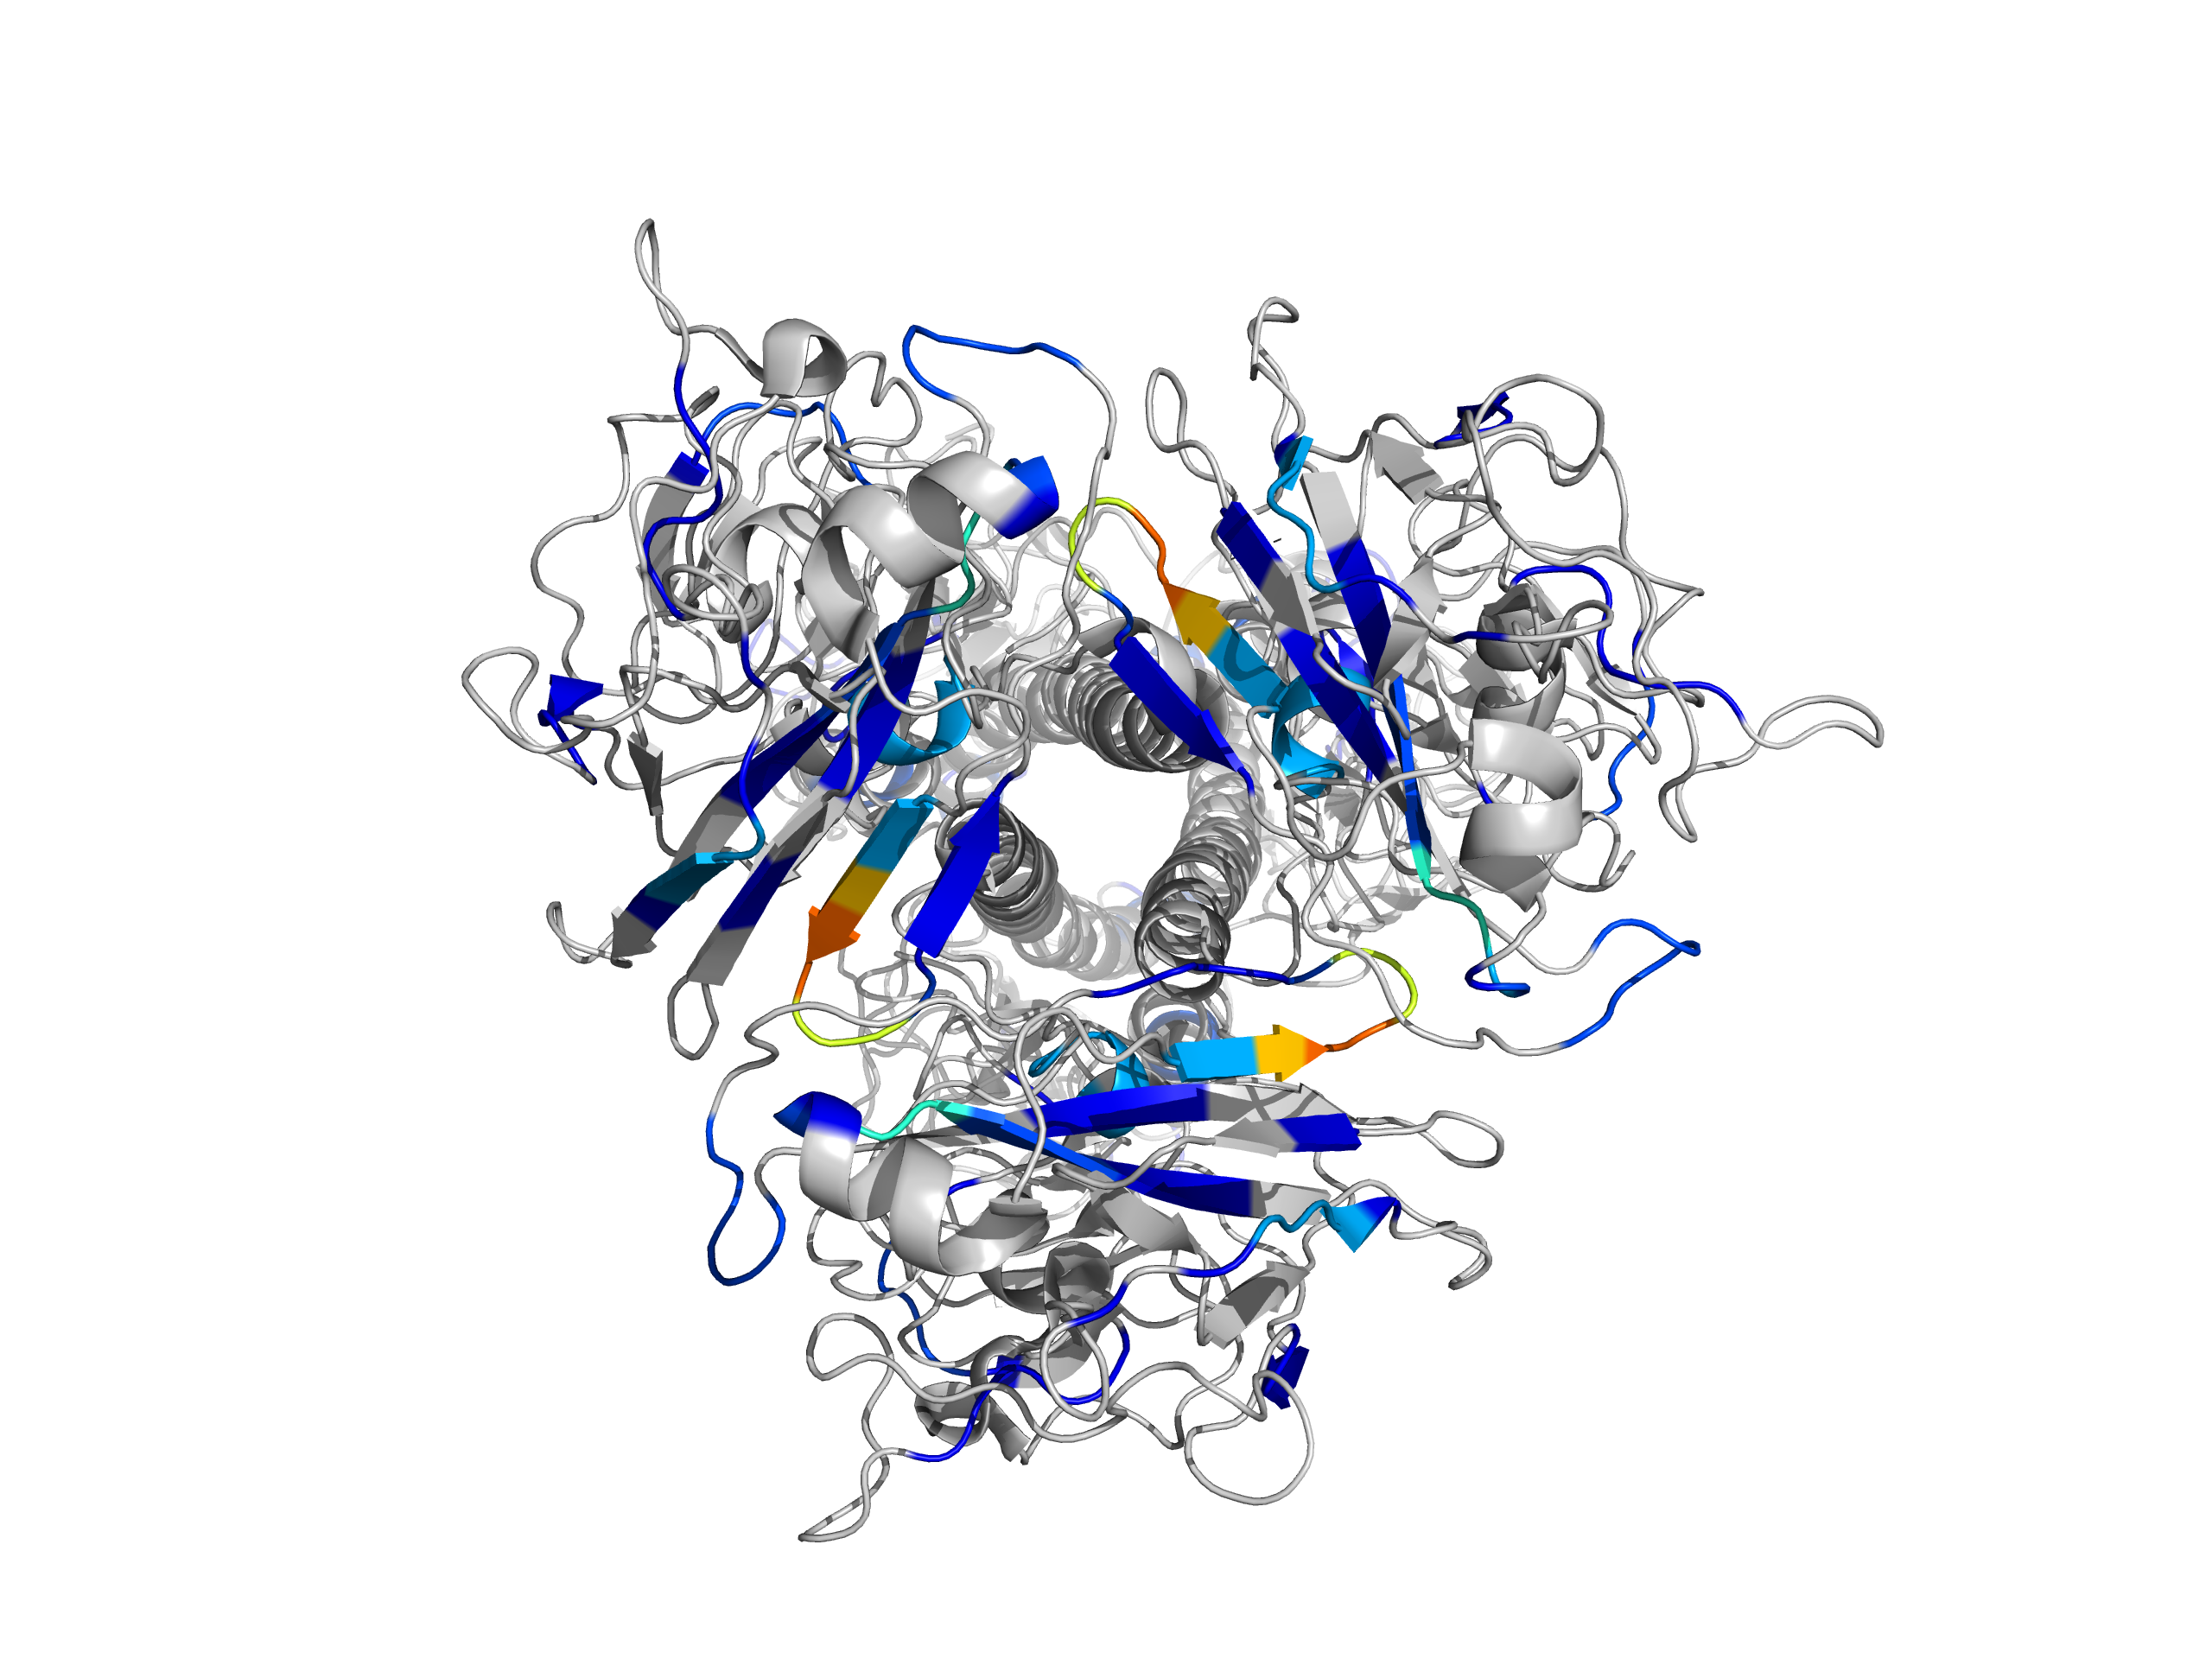
\includegraphics[width=2.75in]{/home/ishanu/ZED/Research/publications/pub_pan_one_/Figures/plotdata/seqanal/ntb/jetrndfile1.png}};
%  \node[anchor=north west] (T111) at ([yshift=-0.15in,xshift=0.05in]T11.south west) {
% 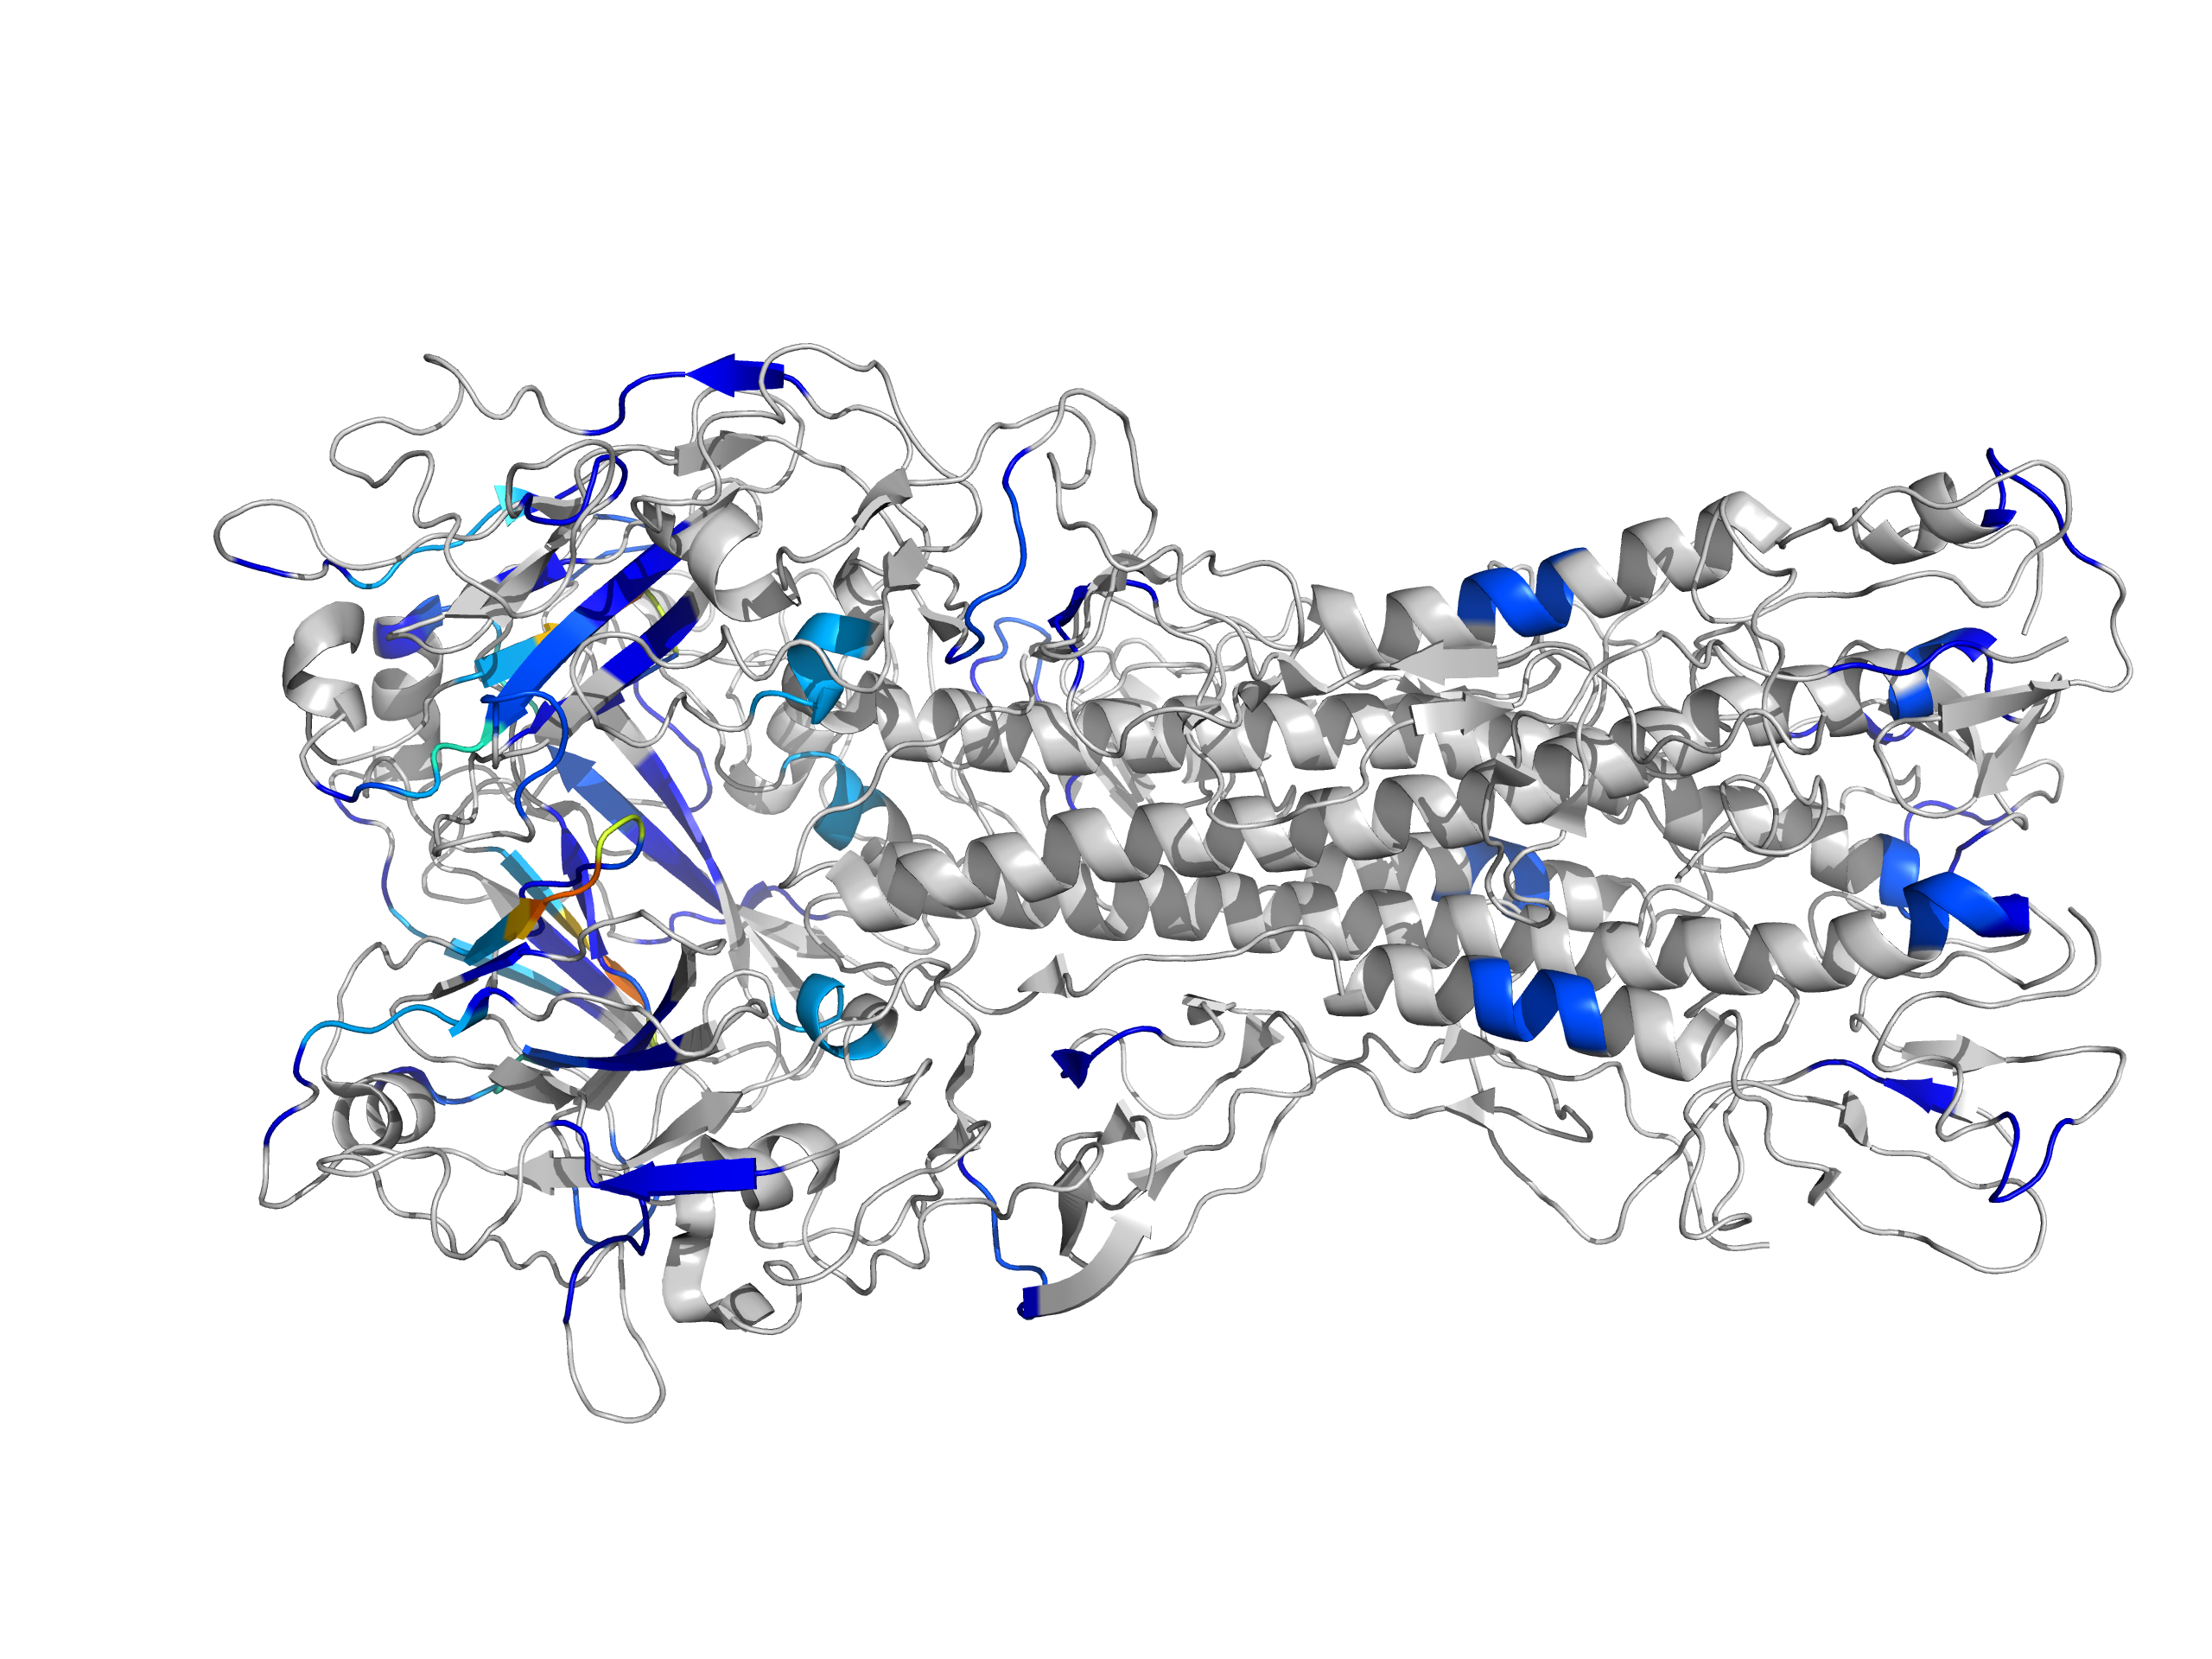
\includegraphics[width=3.5in,angle=-90]{/home/ishanu/ZED/Research/publications/pub_pan_one_/Figures/plotdata/seqanal/ntb/jetrndfile2.png}};
%  \node[anchor=north west] (T112) at ([yshift=0.2in,xshift=.86in]T11.south west) {
% 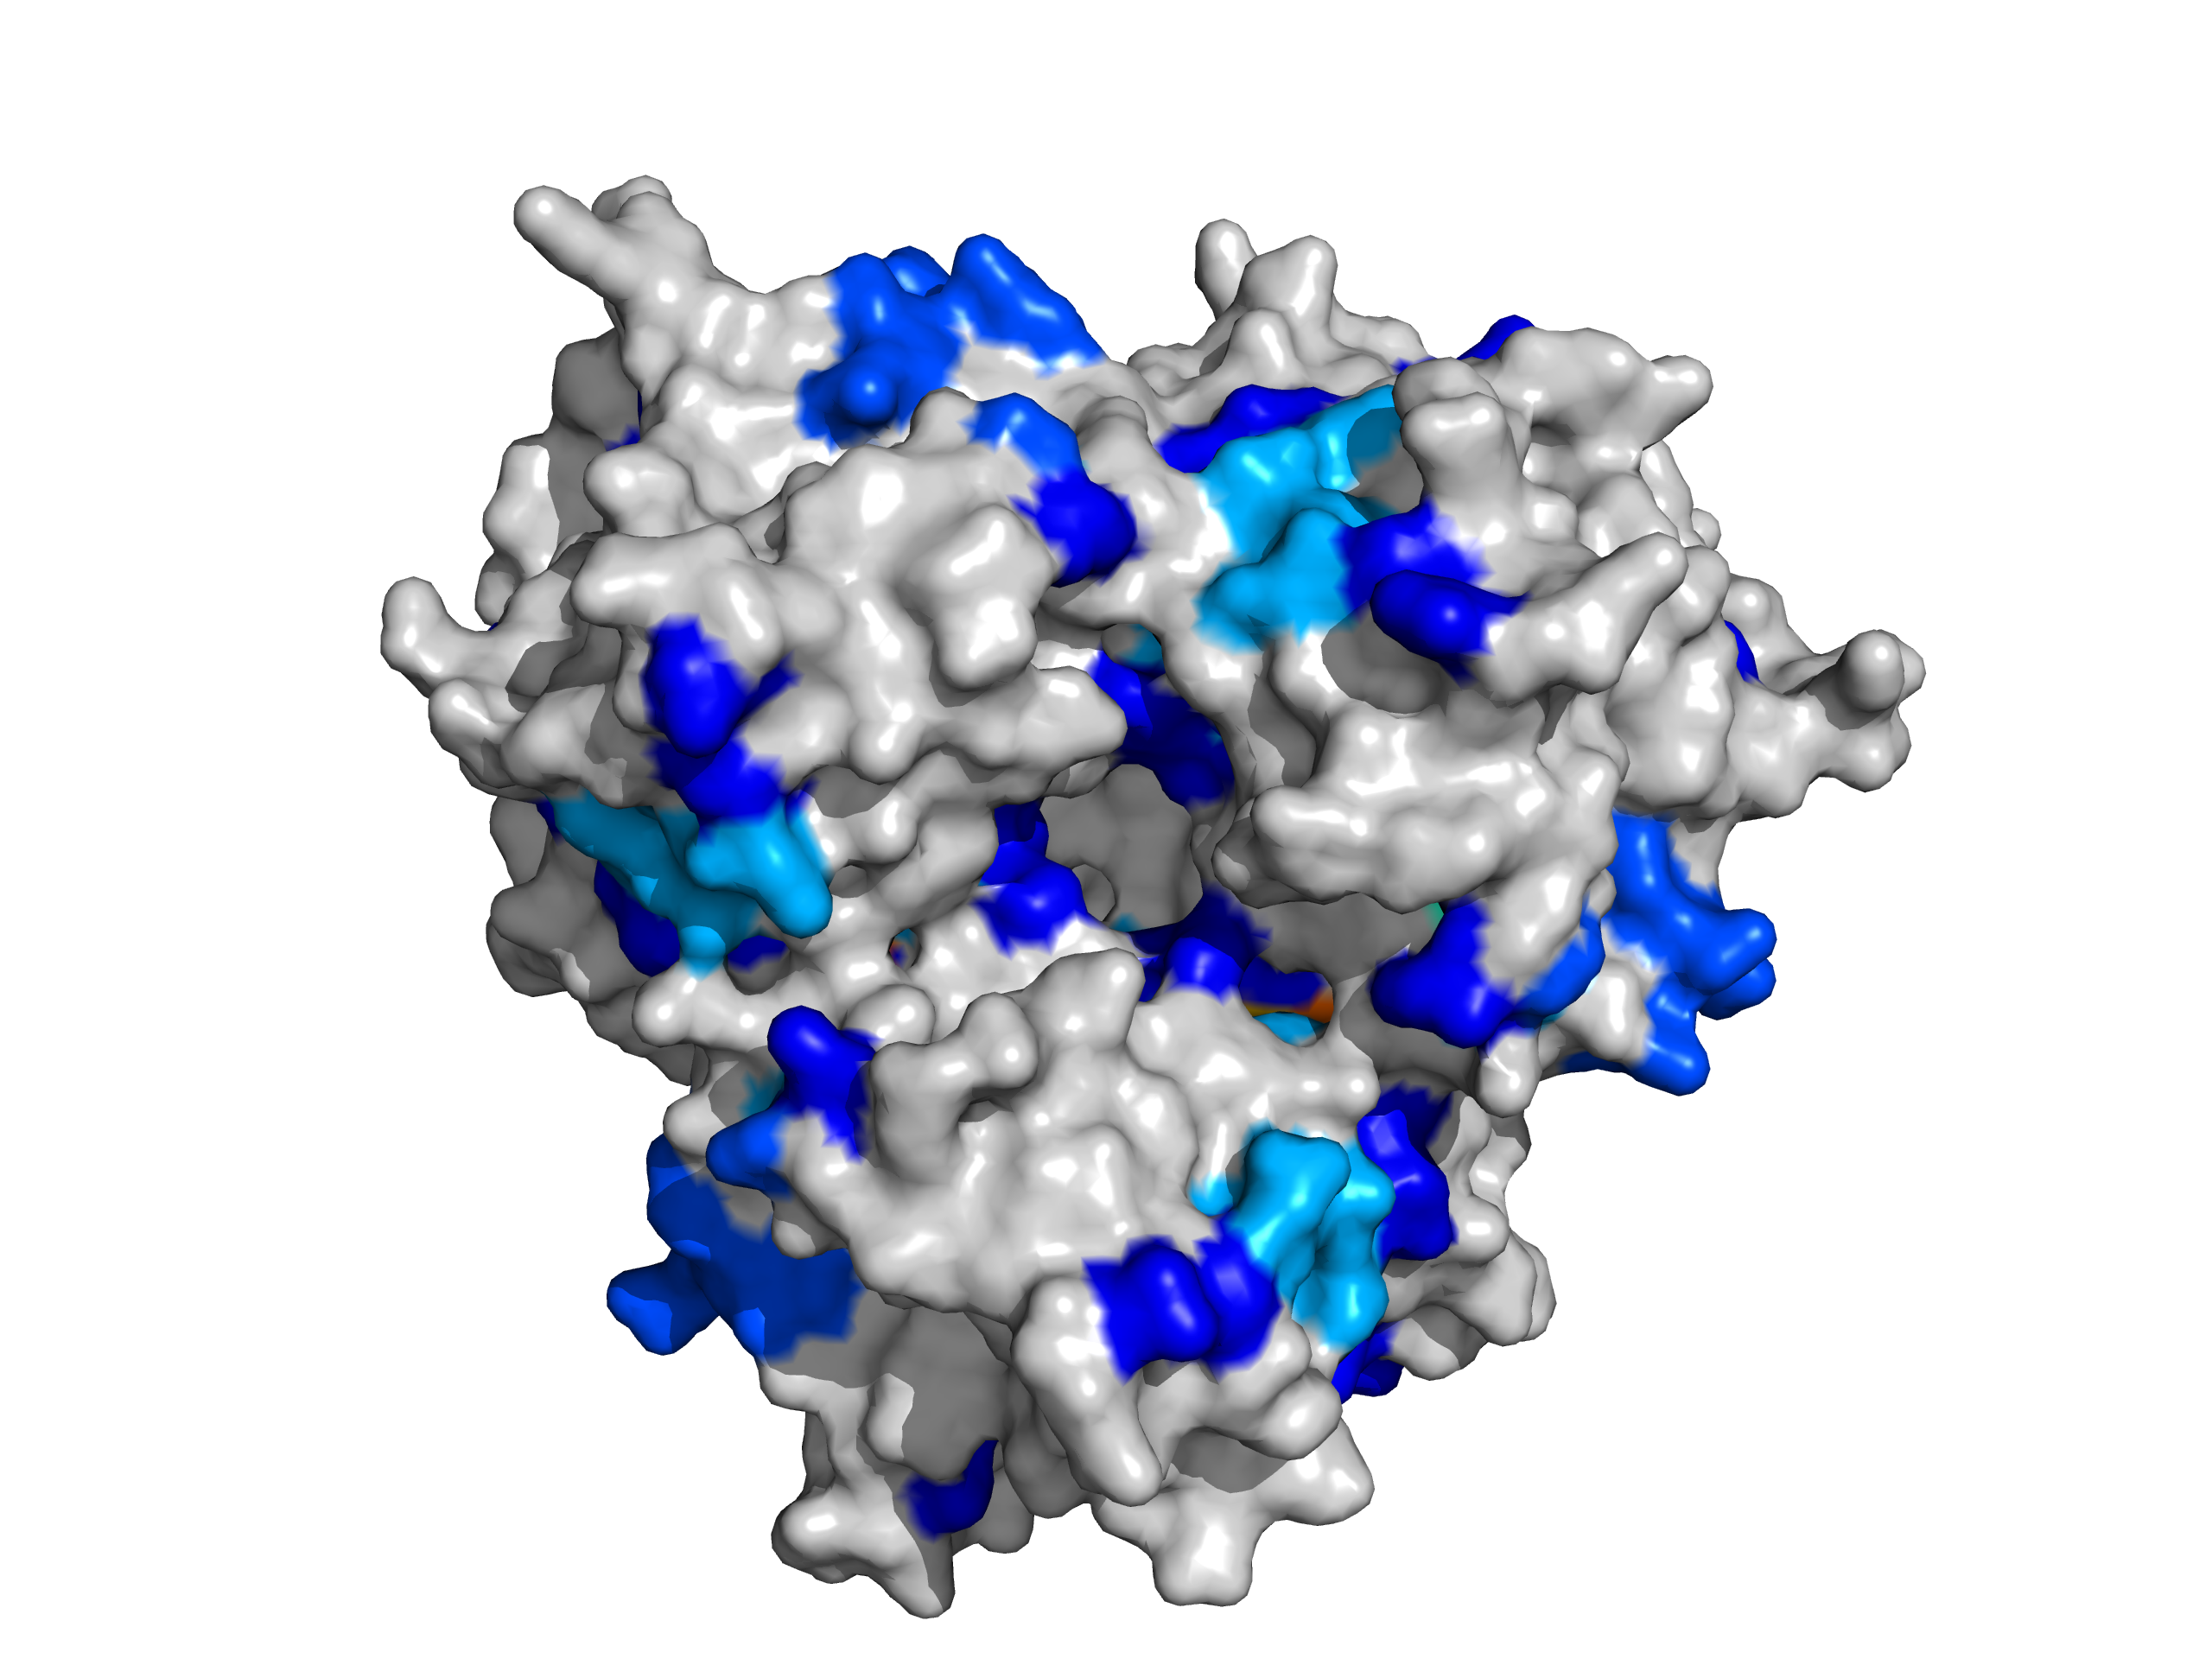
\includegraphics[width=1in]{/home/ishanu/ZED/Research/publications/pub_pan_one_/Figures/plotdata/seqanal/ntb/jetrndfile4.png}};
   

%  \node[anchor=north west] (L2) at ([xshift=.6in,yshift=-0.05in]$(T1.north west)!(T11.west)!(T1.north east)$) {{\large \normalfont g.}};
%  \node[anchor=north west] (L3) at ([xshift=.6in,yshift=-.1in]$(T11.north west)!(T112.north)!(T11.south west)$) {{\large \normalfont h.}};
%  \node[anchor=north west] (L4) at ([xshift=.6in,yshift=-.45in]$(T11.north west)!(T111.north)!(T11.south west)$) {{\large \normalfont i.}};

% \draw [thin, dashed] (T11.center) -- (T111.center);
% \draw [-{latex},thin,Red1] ([xshift=-.8in,yshift=-.5in]T11.center) -- ([xshift=-.38in,yshift=-.17in]T11.center) node [pos=0.1,xshift=-.15in,yshift=-.02in,font=\bf\sffamily\fontsize{6}{6}\selectfont,text=black] {200} ;
% \draw [-{latex},thin,Red1] ([xshift=-.8in,yshift=-.5in]T11.center) -- ([xshift=-0.12in,yshift=-2.1in]T11.center);
% \draw [-{latex},thin,Red1] ([xshift=.6in,yshift=-.65in]T11.center) -- ([xshift=.3in,yshift=-.29in]T11.center) node [pos=-0.15,font=\bf\sffamily\fontsize{6}{6}\selectfont,text=black,fill=white] {200};
% \draw [-{latex},thin,Red1] ([xshift=.1in,yshift=.7in]T11.center) -- ([xshift=.1in,yshift=.34in]T11.center) node [pos=-0.15,font=\bf\sffamily\fontsize{6}{6}\selectfont,text=black,fill=white] {200};

% \draw [-{latex},thin,Red1] ([xshift=.73in,yshift=-.45in]T11.center) -- ([xshift=.7in,yshift=-.2in]T11.center) node [pos=-0.15,font=\bf\sffamily\fontsize{6}{6}\selectfont,text=black,fill=white] {220};

% \draw [-{latex},thin,Red1] ([xshift=.73in,yshift=-.45in]T11.center) -- ([xshift=.7in,yshift=-.2in]T11.center) node [pos=-0.15,font=\bf\sffamily\fontsize{6}{6}\selectfont,text=black,fill=white] {220};

% \draw [-{latex},thin,Red1] ([xshift=.53in,yshift=-.35in]T11.center) -- ([xshift=.42in,yshift=-0.1in]T11.center) node [pos=-0.15,font=\bf\sffamily\fontsize{6}{6}\selectfont,text=black] {180};

% \draw [-{latex},thin,Red1] ([xshift=.53in,yshift=-.35in]T111.center) -- ([xshift=.42in,yshift=-0.6in]T111.center) node [pos=-0.15,xshift=.05in,font=\bf\sffamily\fontsize{6}{6}\selectfont,text=black] {49(HA2)};

% \draw [-{latex},thin,Red1] ([xshift=-.8in,yshift=-.15in]T111.center) -- ([xshift=-.35in,yshift=0.4in]T111.center) node [pos=-0.15,xshift=.05in,font=\bf\sffamily\fontsize{6}{6}\selectfont,text=black] {100};

% \draw [-{latex},thin,Red1] ([xshift=-1in,yshift=.2in]T111.center) -- ([xshift=-.6in,yshift=0.65in]T111.center) node [pos=-0.15,xshift=.05in,font=\bf\sffamily\fontsize{6}{6}\selectfont,text=black] {115};

% \draw [-{latex},thin,Red1] ([xshift=-.8in,yshift=-1.1in]T111.center) -- ([xshift=-0.1in,yshift=-1.32in]T111.center) node [pos=-0.15,xshift=.05in,yshift=.01in,font=\bf\sffamily\fontsize{6}{6}\selectfont,text=black] {124 (HA2)};


  
\end{tikzpicture}
 \else
  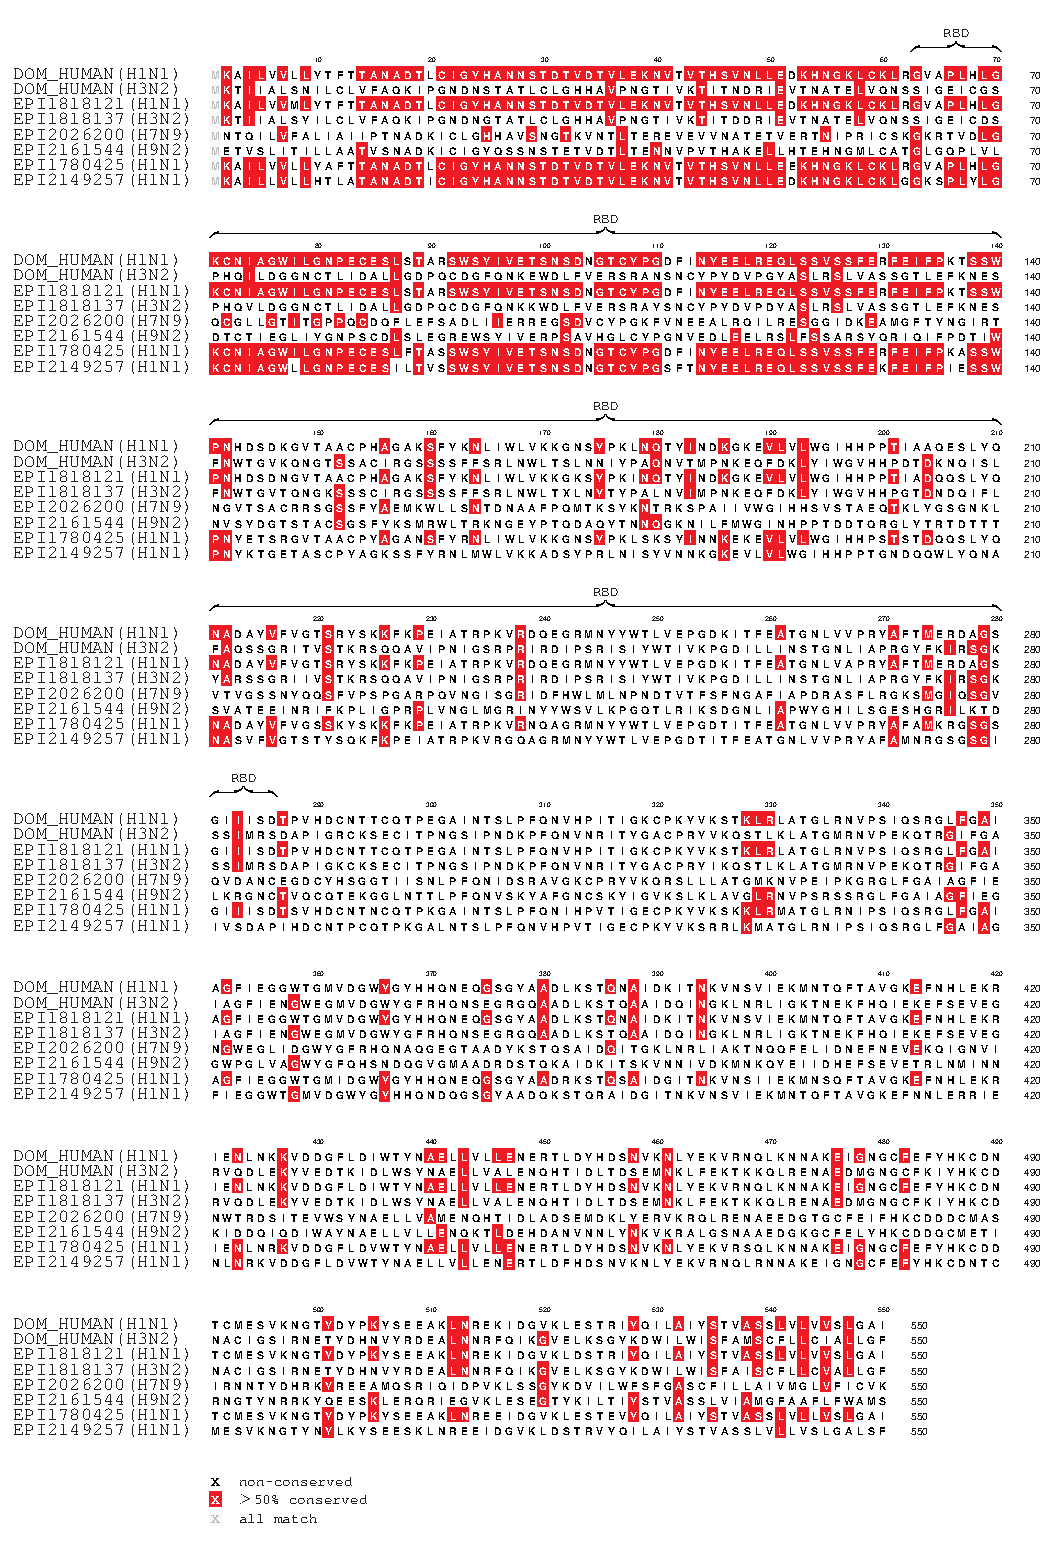
\includegraphics[width=.95\textwidth]{Figures/External/riskyseq}
  \fi 
  \vspace{-18pt}
  
\captionN{HA sequence comparison  with dominant human strains (DOM\_HUMAN H1N1, H3N2)  with \enet estimated top 5 risky strains (2020-2022 April) along with the teh most risky H9N2 strain (A/mink/China/chick embryo/2020), showing substantial differences from the circulating strains both in and out of the RBD. }\label{figriskyseq}
\end{figure}
\else
\refstepcounter{figure}\label{figriskyseq}
\fi



\ifFIGS

\begin{table}[!ht]\centering
\captionN{Count of identified strains above estimated emergence risk threshold}\label{riskytab}

\sffamily\fontsize{7}{8}\selectfont

\begin{tabular}{L{.75in}|L{.25in}|L{.60in}|L{.6in}|L{.6in}|L{.6in}}\hline
subtype | risk&6.0&6.2&6.3&6.4&6.5\\\hline
H1N1&62&57&53&5&4\\
H3N2&11&11&11&4&1\\
H7N9&1&1&1&1&1\\
H9N2&1&1&0&0&0\\
\hline\end{tabular}

\end{table}
\else
\refstepcounter{table}\label{riskytab}
\fi
% #############################################


In addition to  the seasonal flu epidemic posing a serious health concern, novel \infl strains spilling over into humans from animal reservoirs can cause global pandemics, as demonstrated four times (1918 Spanish flu/H1N1, 1957 Asian flu/H2N2, 1968 hongkong flu/H3N2, 2009 swine flu/H1N1) in the past 100 years~\cite{shao2017evolution}. With the memory of sudden emergence of   COVID-19 and the ensuing devastating pandemic fresh in our minds, a looming question  is whether we can prepare for, preempt and mitigate such events in the future.  \infl,  partly on account of its segmented genome and its wide prevalence is common animal hosts, has historically demonstrated its ability to easily incorporate genes from multiple strains and emerge as novel human pathogens~\cite{reid2003origin,vergara2014ns},  thus harboring  a high potential  of triggering the next  pandemic.

A possible approach to mitigating such risk is to identify specific strains in animal hosts that do not yet circulate in humans, but have the potential to spill-over and quickly achieve human-to-human (HH) transmission capability. Despite global surveillance efforts to  collecting wild specimens from diverse hosts and geo-locations, our  current ability to objectively, reliably and scalably  evaluate the risk posed to  humans by  individual animal  strains  is limited.

CDC's current solution to this problem is the Influenza Risk Assessment Tool (IRAT), which  uses a combination of ten weighted risk elements, aiming to factor in the   1) properties of the virus, 2) attributes of the population, and 3) ecology and epidemiological characteristics of the virus~\cite{Influenz24:online} that are largely  expert-selected. The IRAT score assigns  a grade between 1-10 for emergence risk and public health impact to Influenza A viruses not currently circulating among humans. However, evaluating the IRAT risk elements  involve multiple experimental assays for each strain, possibly taking  weeks to return the final   score for a single strain. Thus, we have a scalability problem: while  the current global biosurveillance efforts are collecting tens of thousands of sequences every year, most of these sequences will never be analyzed in time. IRAT assessment protocols are  not fast enough to leverage the full capacity of current surveillance output, and thus have low odds of successfully  preempting a pandemic.

In this study, we introduce a machine learning algorithm to automatically parse out emergent evolutionary constraints operating on \infl viruses in the wild, via analyzing observed variations (point substitutions and indels) of the  amino acid (AA)  sequences  of the two key proteins implicated  in cellular entry and exit~\cite{gamblin2010influenza}, HA and NA respectively. Uncovering and representing these constraints within a predictive framework, which we refer to as the \enet, allows us to estimate the numerical odds of a specific mutation to arise from a given strain  spontaneously in the wild. Explicit quantification of these likelihoods then yields a numerical estimate of the probability of a specific strain of interest giving rise to another. Such numerical estimates are impossible to obtain without first inferring the emergent constraints at play specific to a strain,  as well as  the variation of mutational probabilities from one positional index to the next along the AA sequence. Thus, the many well-known classical  DNA  substitution models~\cite{posada1998modeltest} or standard approaches to phylogenetic tree inference, do not address these issues. 


On account of the fact that  a  strain needs  to be present in sufficiently high numbers in circulation to be  observed and recorded, the sequence data from public databases that we train  with represents strains with high replicative fitness. However, not all variations of the viral genome are equally viable. A lack of proofreading function in influenza viral RNA-polymerase leads to the integration of faulty nucleotides during the viral replication process with a rate of $10^{-3}$ to $10^{-4}$, which results in high mutation rates~\cite{ahlquist2002rna,chen2006avian}. Only specific patterns of such variations can maintain or gain replicative fitness, implying that  the  dependencies between local variations that the \enet uncovers, arises from a  functional necessity of conserving or augmenting  fitness. However, these fitness constraints are not time-invariant. The background distribution of strains, and selection pressure from   long-term evolution of cytotoxic T lymphocyte (CTL) epitopes~\cite{woolthuis2016long,fan2012role,van2016differential,berkhoff2007assessment,van2012evasion} in humans can change quickly. With sufficient number of unique samples to train on for each flu season, the \enet (recomputed for each time-period) is expected to  track these constraints that shape the viral evolutionary trajectories, automatically reflecting the effect of  functional constraints, the impact of constantly evolving host immunity, and the current strain distribution in circulation.  

The ability of the \enet framework to determine the numerical odds of specific sequence variations suggests that we might be able to frame the problem of forecasting future dominant strain(s), and that of estimating the  pandemic potential of an observed animal strain as precise mathematical questions (albeit with some simplifying assumptions), with demonstrated approximate solutions (Fig.~\ref{figscheme}). Thus,  a dominant strain for an upcoming flu season
may be identified as one which maximizes the joint probability of simultaneosly arising from each (or most)  of the currently circulating strains (Fig.~\ref{figscheme}c).
And, a pandemic risk score of a novel strain may be estimated by the probability of it giving rise to a well-adapted human strain.  We validate  our proposed solutions for these problems in out-of-sample data.

\DQS{Add details replacing XXX}
We infer our models using the AA sequences of HA and NA proteins from all available unique \infl strains in the NCBI and GISAID databases between the years XXX to present time (2022 April), which leads to a set of 98XXX strains in total. We only consider strains for which both HA and NA sequences are available, and construct \enet{s} separately for H1N1 and H3N2 subtypes, and for each flu season, constructing in total XXX \enet{s}. %Forecasts of the upcoming  season's dominant strains are made for each flu season for each hemisphere separately.
%
\DQS{add details and example of structure, fixing fig 1 to AA from ATGC}
Structurally, an \enet comprises an interdependent forest of  local predictors: each such predictor aims to model the observed amino acid ``outcome'' at a specific positional index of the protein of interest, using as features   the bases appearing  at other  locations of the protein sequence (Fig.~\ref{figscheme}b). The algorithm automatically identifies the set of features (AA positions) that influence the outcome at a prticular position, implying that an \enet comprises atmost as many such position-specific predictors as the sequence length of the protein. Currently, the component predictors of an \enet are implemented as conditional inference trees~\cite{Hothorn06unbiasedrecursive},% . The inter-dependency between these trees implies that we realize a  recursive collection of decision trees, which in our current implementation are  conditional inference trees~\cite{Hothorn06unbiasedrecursive}
that make sure  each node split during the tree construction has a minimum level of statistical significance in differentiating the resulting child nodes.  %that are%inferred 
% At the core of our algorithmic framework is a recursive forest of  cross-predicting conditional inference trees, which we refer to as the \enet,  
\DQS{WHy dont we use phenotypic information}
Importantly, the \enet component models are inferred purely from the amino acid sequences of the proteins of interest with no additional phenotypic annotation, other than identifying the host animal (and time and place of collection). Despite limiting ourselves to only genotypic information, our approach to probing for deep emergent interdependencies   uncovers a rich structure of fitness-preserving constraints that enable good prediction of future dominant strains. Thus, our modeling approach is a substantial departure from the state of the art; we do not assume models of mutation a priori, and we make use of little information that is specific to \infl genomic sequences, or its life cycle, beyond focusing on HA and NA which are known to be the main targets of neutralizing antibodies~\cite{shao2017evolution}.


% that allows us to  predict the likelihood of specific future  mutations, and  consequently, the numerical likelihood of specific  strains emerging through natural evolutionary processes. Evolutionary trajectories in the wild are shaped by complex hard-to-model selection pressures, and the \enet maximally incorporates the impact of these effects by  learning emergent patterns from public sequence databases.

Our results consist of improved solution to  two important problems described above: 1)  forecast dominant strain(s) for the next flu season, and 2)  identify high risk strains amongst those collected in non-human hosts in the wild. Our \enet-informed forecasts outperform  WHO/CDC recommended flu vaccine compositions almost consistently over the past two decades, for both H1N1 and H3N2 subtypes, individually in the northern and the southern hemispheres. While it is recognized that even well-matched strains can fail to induce a strong immune response due to previous infection history of vaccine recipients~\cite{cobey2018poor}, strain-matching is a crucial component to realizing high vaccine effectiveness~\cite{gouma2020antigenic}. Our results outline a new approach to improve the effectiveness of the flu shot via sophisticated  pattern-recognition, outperforming current practice (WHO/CDC) as well as  recently reported prediction strategies  using more standard computational and/or experimental frameworks~\cite{huddleston2020integrating,neher2014predicting}.
Importantly, our results indicate that \enet-informed forecast algorithm is able to leverage purely sequence information of specific strains, and without using more detailed phenotypic information such deep mutational scanning data~\cite{huddleston2020integrating,neher2014predicting},  improve  predictive performance.

%\DQS{What phenotypic information is used by others}

Our primary claim, however,  is the ability to estimate the pandemic potential of novel strains, via our proposed  \erisk score.  The \erisk score closely tracks  the IRAT estimate for  \infl  viruses, specifically ones that do not yet circulate in humans, and is computable in seconds as opposed to weeks taken by the detailed experimental assays. This dramatic reduction in time and cost potentially opens the door to fully exploiting the  current biosurvellinace capacity, scalably analyzing risk from  the tens of thousands of strains collected every year, and hence moving towards   meaningful preemptive pandemic mitigation strategies.



  {\color{magenta}
    Result requirements:
    0) Check if changes happen on incorporating the additional term from eqn 9
    
    1) percent improvement data table augnment with comparison against literature data (in number of average mutational deviation)
    
    2) table for fig 2
    
    3) table/figure for risk scores of all h3n2/h1n1 strains in swine collected in 2021/2022
    
    4) How many sequences were used from which databases. Where is this info described (need this to appear in teh abstract as well)
    
    5) all qnets should be submitted to zenodo


    It seems the old results were generated using a different version of quasinet package. Maybe we should indeed regenerate the results to make sure we can answer reviewer questions.

    Target results:

    1. HA NA recommendations, northern outhern hemispheres (earlier we used 2 years of data, and chose the time over which we consider last season sequences as different for north vs the south, we did not use separate qnets over north/south)

    2. check if recommendations match or errors match at least
    3. check similar approach for latest years
    4. must complete IRAT prediction table (using geometric mean between ha and na estimates seems to do better. try)


  }


\section*{Results}

We begin by collecting  $>98,000$ Influenza A HA/NA nucleotide sequences from two public databases (NCBI:  \href{https://www.ncbi.nlm.nih.gov/genome/viruses/}{https: //www.ncbi.nlm.nih.gov/genome/viruses/}
and GISAID:  \href{https://www.gisaid.org/}{https://www.gisaid.org/}
see SI-Table~\ref{SI-tabseq}), uncovering a network of  dependencies between individual mutations revealed through subtle variations of the aligned sequences. The representation of these dependencies as a recursive forest of conditional inference trees is referred to as the \enet (see Fig.~\ref{figscheme}). 
%
\DQS{update the index refs}Using aligned genomic sequences sampled from  similar populations, $e.g.$ HA from Human Influenza A in year 2008, we  learn models for predicting the mutational variations at each sequence index using other indices  as features. For example, in Fig.~\ref{fig0}a,  the predictor for index 1274 uses variation at index 1064 as a feature, and the predictor for index 1064 uses index 1314 as a feature, and so on -- ultimately uncovering a recursive dependency structure. The \qnet predicts the nucleotide distribution over the base alphabet at any specific index, conditioned on the nucleotides making up the rest of the sequence of the gene or genome fragment under consideration. Aside from this example, amino acids sequences can also be used to train the \qnet.

Finally, we define the q-distance (see Eq.~\eqref{q-distance} in Materials and Methods) as the square-root of the Jensen-Shannon (JS) divergence~\cite{cover} of these conditional distributions from one sequence to another, averaged over the entire sequence. The q-distance, informed by the dependencies modeled by the inferred {\qnet}s, adapts to the specific organism, allele frequencies, and variations in the background population. Invoking Sanov's theorem on large deviations~\cite{cover}, we show  that the  likelihood of spontaneous change is bounded above and below by a simple exponential function of the  q-distance. 

% The mathematical intuition behind relating the new distance to change-probability  is the same as in the prediction of  a biased outcome when we sequentially toss a fair coin. With an overwhelming probability, such an experiment with a fair coin should result in roughly equal number of heads and tails. However, ``large deviations'' can happen, and the probability of such rare events is quantifiable~\cite{varadhan2010large} with existing theory. We show here that the likelihood of a spontaneous transition of a genomic sequence to a  different variant by random chance may also be similarly bounded, given we have the \qnet as  an estimated model of the evolutionary constraints.

Importantly, the q-distance  between two sequences may change even if only the background population changes (see SI-Table~\ref{SI-tabex}, where  the distance between two  fixed sequences vary when we vary their collection years). Sequences may have a large q-distance and a small edit distance, and vice versa (although on average the two distances tend to be positively correlated, see SI-Table~\ref{SI-tabcor}).  Hence for tracking drift in Influenza A, we construct a seasonal \qnet for each sub-type and protein that we consider.

Our first application aims to predict dominant strains for the seasonal flu epidemic. Periodic adjustment of the Influenza vaccine components is necessary to account for antigenic drift~\cite{boni2008vaccination,dos2016influenza}. The flu shot in each hemisphere is annually prepared at least six months in advance, and is based on a cocktail of historical strains determined by the WHO via global surveillance~\cite{agor2018models}, hoping to match the circulating strain(s) in the upcoming flu season. A variety of hard-to-model effects hinder this prediction, which, despite observed cross-reactive effects~\cite{tricco2013comparing}, have limited vaccine effectiveness in recent years~\cite{cdceff}.

%For predicting future strains, we hypothesized that since the probability of a drift exponentially decreases with an increasing q-distance, the centroid of the strain distribution in our metric will change slowly. If true, the strain selected closest to the ``q''-centroid will be a good approximation of next season's dominant strain.

We then computed the dominant strain in each season as the centroid of the strain distribution observed in a given season in the classical sense (no. of mutations), since the edit distance metric is widely used and offers a point of comparison between WHO predictions and \qnet predictions. Note that the recommendations for the northern hemisphere are given in February, while that for the southern hemisphere are given at the end of December the previous year, keeping in mind that the flu season in the south begins a few months early, as described in Fig.~\ref{figseasonal}. Finally, we computed the edit distance (no. of mutations) between the dominant strain and the WHO and \qnet predictions.

Our second application aims to compare emergence risk grades given by the CDC through its Influenza Risk Assessment Tool (IRAT) with results using our q-distance metric. While IRAT uses a combination of 10 weighted risk elements evaluated slowly over the course of several months per strain, we attempt to quantify emergence risk quickly with the q-distance metric. We looked at the same strains that were analyzed by IRAT. For each strain previously analyzed by IRAT, we construct \qnet models for HA and NA segments using all human strains of the same variety circulating in the year prior to risk assessment. For example, the "A/swine/Shandong/1207/2016" strain was assessed by IRAT in July 2020, so we will use human H1N1 strains circulating between July 1, 2019 through June 30, 2020. For sub-types with few human strains (H1N2, H5N1, H5N6, H7N7, H9N2), we only use the upper bound of the date. We then compute the average q-distance between the strain in question and the circulating human strains for both HA and HA segments. Seven of the 23 strains are not included in our comparison due to having zero or too few human strains in the sample space to construct a \qnet; see Supplementary Text, SI-Table~\ref{SI-irattab}. We hypothesize that a lower average q-distance between the strain in question and circulating human strains should correspond to a higher emergence risk. Hence, we expect to see a high negative correlation between q-distance and IRAT grade, which assigns 1 to be the lowest risk and 10 to be the highest risk.

\subsection*{Concrete Results} 

We tested the hypothesis of our first application, computing the strain closest to the ``q''-centroid for each flu season and selecting that strain as the prediction for the next season's dominant strain. We performed this analysis on past two decades of sequence data for Influenza A (H1N1 and H3N2) with promising results: the q-distance based prediction demonstrably outperforms WHO recommendations by reducing  the  distance between the predicted and  the dominant  strain (Fig.~\ref{figseasonal}). Recall that we identify the dominant strain to be the one that occurs most frequently, computed as the centroid of the strain distribution observed in a given season in the classical sense (no. of mutations).

The \qnet single-cluster predictions consistently outperform the WHO recommendations. For H1N1 HA, the \qnet induced recommendation outperforms the WHO suggestion by $>33\%$ on average over the last two decades, and $>71\%$ on average in the last decade. The gains for H1N1 NA over the same time periods are $>15\%$ and $>52\%$, respectively. For H3N2 HA, the \qnet induced recommendation outperforms the WHO suggestion by $>37\%$ on average over the last two decades, and $>40\%$ in the last decade. The gains for H3N2 NA over the same time periods are $>14\%$ and $>15\%$, respectively. Finding multi-cluster predictions has the potential to yield even more improved results, as seen in Fig.~\ref{figseasonal} and SI-Table~\ref{SI-tabrec8} through SI-Table~\ref{SI-tabrec11}.

The full table of single-cluster results with improvement broken down by hemisphere is given in Table~\ref{tabperf}. Fig.~\ref{figseasonal} illustrates the relative gains computed for both subtypes and the two hemispheres (since the flu season occupy distinct time periods and may have different dominant strains in the northern and southern hemispheres~\cite{boni2008vaccination}). Additional improvement is possible if we recommend multiple strains every season for the vaccine cocktail (Fig.~\ref{figseasonal}e,f,k,l). The details of the specific strain  recommendations made by the \qnet approach for two subtypes (H1N1, H3N2), for two genes (HA, NA) and for the northern and the southern hemispheres over the previous two decades are enumerated in the Supplementary Text in Tables SI-Table~\ref{SI-tabrec0} through SI-Table~\ref{SI-tabrec11}.

We hypothesized in our second application that there will be a high negative correlation between q-distance and IRAT emergence grade. Plotting our results in Fig.~\ref{figirat}, we find a correlation of $-0.7032$ $(p < 0.005)$, which is statistically and substantively significant. We can conclude, therefore, that a lower averae q-distance to currently circulating human strains corresponds to a higher risk of emergence with respect to the CDC's grades. Due to the small number of Influenza A strains that have been analyzed by IRAT, we should be wary of the realistic statistical significance of our results. Achieving a moderately high correlation coefficient and p-value is nevertheless a positive result, and further uncovers the potential of our model to quantify risk of emergence. 

For further analysis, we also performed q-analysis on IRAT H1- and H3- sub-types by taking average q-distance between the target strain and all human-circulating strains available, with no upper or lower collection date bound. We expected the correlation to be worse than with bounded strains, since a strain being ``close" to humans at some point in the past does not necessarily mean being close now. Indeed, our results showed almost no correlation to the IRAT emergence risk scores. Bounded results for H1- and H3- sub-types yielded a correlation of $-0.6916$, while unbounded results yielded a correlation of $0.0545$; see SI-Fig.~\ref{SI-irat}.

Given the efficiency of the q-distance computations, we can track how risk of emergence changes over time by continually updating the current human-circulating strains each year. For exact average q-distance and \qnet sample size statistics, please see SI-Table~\ref{SI-irattab} in the Supplementary Text.

\section*{Discussion}

\subsection*{\enet Advantages and Related Literature}

Numerous tools exist for ad hoc quantification of genomic similarity~\cite{posada1998modeltest,goldberger2005genomic,huelsenbeck1997phylogeny,neher2014predicting,VanderMeer2010,Smith2009}, which are not inherently biologically meaningful -- a smaller edit distance between two strains does not necessarily imply that a feasible trajectory exists from one to the other in the wild. These measures tend to be  variations of distances between symbolic sequences, and are not aware of selection pressures and evolutionary dynamics. Despite the diverse techniques and concepts explored in these domains, the key missing piece is effectively learning which changes are likely in the wild, conditioned on possibly the entire sequence of the current strain. Our algorithm is the first of its kind to learn an appropriate metric of comparison from data, without assuming any model of DNA or amino acid substitution, or a genealogical tree a priori, and is  designed to be aware of the impact of the  host environment and background epidemiology.


This is a major improvement over the existing state of art in phylogeny construction from sequences, which generally assume a model for character substitution (either for nucleotides or amino acid residues) ignoring the effect of selection and the existence of long-range complex dependencies in viable mutations along the genomic sequence. Notably, even relatively complex substitution models ($e.g.$ ones that allow site specific mutation rates) do not capture the effect of individual changes that may dramatically alter fitness in the environment. Our proposed approach, on the other hand, learns from and leverages these patterns, using sophisticated pattern discovery via novel machine learning algorithms. While the effect of the environment and selection cannot be inferred from a single sequence, an entire database of observed strains, processed through sophisticated learning, can parse out predictive models of these complex interactions. Our only intuitively well-justified assumption on the evolutionary dynamics is that more fit strains end up with more progenies (follows from definition of Malthusian fitness), and are thus more likely to be sampled in surveillance efforts (again, intuitively obvious).  Thus, in a strict mathematical sense, the distance we propose is not a distance between two strains $x,y$, but a distance between strain $x^A$ ($x$ in a background environment $A$) and a strain  $y^B$ ($y$ in a background environment $B$). Indeed we can show that the distance between the same pair of  strains of \infl HA is different based on if they are collected in 2008 vs in 2009, reflecting that the background environment and circulating diversity changed over the two years.  Thus, our  distance metric  is fundamentally different from measures that exist in the literature. In particular, our mathematical framework leads to the key result that the q-distance is a scaled representation of the log-likelihood of spontaneous jump  between strains. This interpretation is missing in existing tools, and makes way for leveraging the q-distance to model emergence of new strains. Thus, we can predict entirely new sequences -- which differ by a non-trivial number of edits from any observed strain -- that still lead to functional proteins, as demonstrated in our preliminary studies.

Very recently, two articles have explored the possibility of predicting  pathogenicity from genomic sequences (Mollentze~\cite{mollentze2021identifying}) and forecasting which amongst observed mutations will dominate the circulating population (Maher et al~\cite{maher2021predicting}). These studies provide strong pieces of evidence that challenge the idea that forecasting future variants of virus strains is impossible, while aligns with our goals. While their questions overlap with our framework, our approach is distinct and more ambitious. For example,  Mollentze  uses  classical  sequence similarity; extended to include similarity to  human housekeeping genes hoping to identify viruses  evading the human immune system more easily.  The demonstrated  performance is poor (incorrectly tagging all SARS-related coronaviruses as potentially pathogenic), implying un-actionable specificity. On the other hand,  Maher outright assumes mutations to be independent. Features are found manually,  are specific to \hcov, and the authors take  a meta-analysis-esque route, compiling together a ``kitchen-sink'' of features via standard machine learning. Importantly, these approaches  only aim to predict point mutations, with  the gargantuan complexity of tracking a more complete strain through a high-dimensional sequence space well beyond their conceptual limits. Thus, even the question if whether a yet-to-be-seen strain is indeed a valid biological encoding of a virus (which is simpler to determining risk posed by such future variants) cannot answered by our peers, limiting such approaches to analyzing mutations already seen, or strains  already collected.  Additionally, generalizability and actionability is  suspect, given that Maher's features are \hcov specific, and Mollentze's similarity to house-keeping genes might not be universal. Finally, both these  approaches apply to a mutation or a combination of mutations that already exist, and cannot predict new mutations, or new strains.




{\color{Red1}
\section*{Discussion}
In the aftermath of the COVID-19 pandemic that caused one of the most devastating disasters of the past century, a looming question is whether we can prepare for, preempt and mitigate such events in the future. Evolving viruses, whether currently circulating in the human population, or in animal reservoirs that might spillover and attain human-to-human transmission capability, pose an ever-present epidemic risk.  Current surveillance paradigms, while crucial for mapping disease ecosystems, are limited in their ability to address this challenge. Habitat encroachment, climate change, and other ecological factors~\cite{rulli2017nexus,chua2002anthropogenic,childs2004zoonotic} unquestionably drive up the odds of zoonotic spill-overs. Nevertheless, current efforts at tracking these effects have not improved our ability to quantify future risk of emergence~\cite{fair2019viral}. Tracking viral diversity in animal hosts, while important, often does not transparently map to emergence risk.  This is particularly true for \infl, which partly on account of its segmented genome, can easily incorporate genes from multiple strains and emerge as novel human pathogens, and thus harbor a high pandemic potential. While large antigenic shifts in \infl are relatively rare, even the smaller seasonal sequence alterations in cause sufficient variation in the surface proteins to evade existing immunity, and require yearly reformulation of the flu vaccine.

However, for the  vaccine to be effective, we need to  predict the dominant circulating strain of the upcoming season with sufficient accuracy.
Currently, the composition of the flu shot is decided at least six months in advance of the seasonal infection peak, and targets three to four  historical strains as recommended by the CDC/WHO, who identify these specific strains by  sampling the current circulation~\cite{agor2018models}, hoping to match the  dominant strain(s) in the upcoming season. A variety of hard-to-model effects hinder this prediction, which, despite observed cross-reactive effects~\cite{tricco2013comparing}, have had  limited vaccine effectiveness in recent years~\cite{cdceff}. Rank-ordering strains which do not yet circulate in humans according to either their spillover risk or their pandemic potential, has proven to be even more difficult [REF]. CDC's current, somewhat subjective, solution to this problem is the Influenza Risk Assessment Tool (IRAT), which  uses a combination of ten weighted risk elements, including  1) properties of the virus, 2) attributes of the population, and 3) ecology and epidemiological characteristics of the virus~\cite{Influenz24:online} that are expert-selected. Evaluating these factors involve several experimental assay for each strain, taking possibly weeks to return the final IRAT  score for a single strain. Thus, we have a scalability problem: with  the current global biosurveillance efforts  collecting tens of thousands of sequences every year, IRAT assessment is simply not fast enough to  preempt a pandemic. }

 

\section*{Discussion \& Sequence Comparisons}

For further discussion, we looked at our \qnet predictions more closely. Comparing the \qnet inferred strain (QNT) against the one recommended by the WHO, we find: 1) the residues that only the QNT matches correctly with DOM (while the WHO fails) are largely localized within the receptor binding domain (RBD), with $>57\%$ occurring within  the RBD on average (see Fig.~\ref{figseq}a for a specific example), and 2) when the WHO strain deviates from  the QNT/DOM  matched residue, the ``correct'' residue is often replaced in the WHO recommendation with one that has very different side chain, hydropathy  and/or chemical properties (see Fig.~\ref{figseq}b-f), suggesting deviations in recognition characteristics. Combined with the fact that we find circulating strains are almost always within a few edits of the DOM (see SI-Fig.~\ref{SI-figdom}), these observations suggest that hosts vaccinated with the QNT recommendation is more likely to have season-specific antibodies that are more likely to recognize a larger cross-section of the circulating strains.

High season-to-season genomic variation in the key  Influenza capsidic proteins is driven by two opposing influences: 1) the need to conserve function  limiting random mutations, and 2) hyper-variability to escape recognition by neutralizing antibodies. Even a  single residue change in the surface proteins might dramatically alter recognition characteristics, brought about by unpredictable~\cite{carugo2001normalized,righetto2014comparative} changes in local or regional properties such as charge, hydropathy, side chain solvent accessibility~\cite{lee1971interpretation,shrake1973environment,momen2008impact,adamczak2005combining}.

Focusing on the average localization of the QNT to WHO deviations in the HA molecular  structure, the changes are observed to primarily occur in the HA1 sub-unit (see Fig.~\ref{figseq}g-i, HA0 numbering used, other numbering conversions are given in SI-Table~\ref{SI-tabnum}), with the most frequent deviations  occurring around the $\approx 200$ loop, the $\approx 220$ loop, the $\approx 180$ helix, and the $\approx 100$ helix, in addition to some residues in the HA2 sub-unit ($\approx 49$ \& $\approx 124$). Unsurprisingly, the residues we find to be most impacted in the HA1 sub-unit (the globular top of the fusion protein) have been repeatedly implicated in receptor binding interactions~\cite{tzarum2015structure,lazniewski2018structural,garcia2015dynamic}. Thus, we are able to fine tune the future recommendation over the state of the art, largely by modifying residue recommendations around the RBD and  structures affecting recognition dynamics.





\section*{Limitations \& Conclusion}

Calculation of q-distance  is currently limited to similar and aligned sequences, $e.g.$  Influenza strains from different sub-types, hosts or seasons. Furthermore, we need a sufficient diversity of observed strains to successfully construct the \qnet. A multi-variate regression analysis indicates  that the most important factor for our approach to succeed is  the diversity of the sequence dataset (see Supplementary Text, SI Table~\ref{SI-tabreg}). Arguably, simply reducing the edit distance from the dominant strain is not guaranteed to translate to a better immunological protection. Nevertheless, consistent improvement in this metric achieved purely via computational means suggests the possibility of improvement over current practice. 

In conclusion, we introduce a data-driven distance metric to track subtle deviations in sequences. We show that we can use the q-distance metric to make recommendations for the flu-shot composition, outperforming the WHO's recommendations in relation to the dominant strain. We also show that we can roughly replicate the CDC's IRAT grades for emergence risk of strains not currently circulating among humans in an efficient manner that can be scaled to rank many more strains than is currently done. The ability to predict future flu strains via subtle variations in a limited set of immunologically important residues suggest that the tools developed here could lead to more effective escape-resistant vaccines, which could be essential in preempting and mitigating the next pandemic.



\section*{Online Methods}


\allowdisplaybreaks{
We briefly describe the proposed computational framework. 


\subsection*{\enet Framework}
We do not assume that the mutational  variations at the individual indices of a genomic sequence are independent (See Fig~\ref{figscheme}a). Irrespective of whether mutations are truly random~\cite{hernandez2018algorithmically}, since only certain combinations of individual mutations are viable, individual mutations across a genomic sequence replicating in the wild  appear  constrained, which is what is explicitly  modeled in our approach.

% 

Consider a set of random variables $X=\{X_i\}$, with $i \in \{1, \cdots, N\}$, each taking value from the respective sets $\Sigma_i$. Here each $X_i$ is the random variable modeling the ``outcome'' $i.e.$ the AA residue at the $i^{th}$ index of the protein sequence. A sample $x \in \prod_1^N \Sigma_i$ is an ordered $N$-tuple, which is a specific strain in this context,  consisting of a realization of each of the variables $X_i$ with the $i^{th}$ entry $x_i$ being the realization of random variable $X_i$.

We use the notation $x_{-i}$ and $x^{i,\sigma}$ to denote:
\begin{subequations}\cgather{
x_{-i} \triangleq x_1, \cdots, x_{i-1},x_{i+1},\cdots,x_N\\
x^{i,\sigma} \triangleq x_1, \cdots, x_{i-1},\sigma,x_{i+1},\cdots,x_N, \sigma \in \Sigma_i
}\end{subequations} Also, $\Dx(S)$ denotes the set of probability measures on  a set $S$, $e.g.$,  $\D$ is the set of  distributions on  $\Sigma_i$.

We note that $X$ defines a random field~\cite{vanmarcke2010random} over the index set $\{1, \cdots, N\}$. 

\begin{defn}[\enet]
For a random field $X=\{X_i\}$ indexed by $i \in \{1, \cdots, N\}$, the \enet is defined to be the set of predictors $\Phi=\{\qn\}$, $i.e.$, we have:
\cgather{
\qn : \prod_{j \neq i} \Sigma_j \rightarrow \D,
}  where for a sequence $x$, $\Phi_i(x_{-i}) $ estimates the distribution of $X_i$ on the set $\Sigma_i$.
\end{defn}
We use conditional inference trees as models for predictors~\cite{Hothorn06unbiasedrecursive}, although more general models are possible.





\subsection*{Biology-Aware Distance Between Sequences}
The mathematical form of our metric is not arbitrary; JS divergence is a symmetricised version of the more common KL divergence~\cite{cover} between distributions, and among  different possibilities, the \qdist  is the simplest metric such that the likelihood of a spontaneous jump (See Eq.~\eqref{fundeq} in Methods) is provably bounded above and below  by simple exponential functions of the \qdist.

\begin{defn}[\qdist: adaptive biologically meaningful dissimilarity between sequences]\label{defqdistance}
Given two sequences $x,y \in \prod_1^N\Sigma_i$, such that $x,y$ are drawn from the  populations $P,Q$  inducing the \enet $\Phi^P,\Phi^Q$, respectively,  we define a pseudo-metric $\theta(x,y) $, as follows:
\cgather{\label{q-distance}
\theta(x,y) \triangleq \mathbf{E}_i \left (  \J^{\frac{1}{2}} \left (\qn^P(x_{-i}) , \qn^Q(y_{-i})\right ) \right )
} 
where $ \J(\cdot,\cdot)$ is the Jensen-Shannon divergence~\cite{manning1999foundations} and $\mathbf{E}_i$ indicates expectation over the indices.
\end{defn}
The square-root in the definition arises naturally from the bounds we are able to prove, and is dictated by the form of Pinsker's inequality~\cite{cover}, ensuring that   the sum of the length of successive path fragments equates the length of the path.%, making it possible to use standard  algorithms  for q-phylogeny construction.


%\subsection*{Significance Test for Population Membership}
\subsection*{Membership Degree}

For our modeling to be reliable, we need a quantitative test of how well the \enet represents the data. Here, we formulate an explicit membership test to ascertain if individual samples may indeed be generated by the \enet with sufficiently high probability.
%
\begin{defn}[Membership probability of a sequence]\label{defmem}
Given a population $P$ inducing the \enet $\Phi^P$ and a sequence $x$, we can compute the membership probability of $x$:
\cgather{
\mem{x}^P \triangleq Pr(x \in P) = \prod_{j=1}^N \left ( \Phi^P_j(x_{-j}) \vert_{x_j} \right )
}
\end{defn}
$x_j$ is the $j^{th}$ entry in $x$, and is thus an element in the set $\Sigma_j$. Since we are mostly concerned with the case where $\Sigma_j$ is a finite set, $\Phi^P_j(x_{-j}) \vert_{x_j}$ is the entry in the probability mass function corresponding to the element of $\Sigma_j$ which appears at the  $j^{th}$ index in sequence $x$. 
 
We can carry out this calculation for a sequence $x$  known to be in the population $P$ as well, which allows us to define the membership degree $\M^P_x$.
\begin{defn}[Membership degree]
Let $X$ be a random field representing a population $P$, $ie.$. $X=x$ is a randomly drawn sequence from $P$. Then  the membership degree $\M^P$ is  a function of the random variable $X$: 
\cgather{
\M^P(X)  \triangleq  \prod_{j=1}^N \left ( \Phi^P_j(X_{-j}) \vert_{X_j} \right )
}Note that $\M^P$ takes values in the unit interval $[0,1]$, and the probability  $x$ is a member of the population $P$ is $\M^P(X=x)$, denoted briefly as $\mem{x}^P$ or $\mem{x}$ if $P$ is clear from context.
\end{defn}
Since $\M^P(X)$ is a random variable, we can now compute sets of sequences that better represent the population $P$, and ones that are on the fringe. We can also evaluate using a pre-specified significance-level if a particular sequence is not from the population $P$.



\subsection*{Theoretical Probability Bounds}

The \enet framework  allows us to rigorously compute bounds on the probability of a spontaneous change of one strain to another, brought about by chance mutations. While any sequence of mutations is equally likely, the ``fitness'' of the resultant strain, or the probability that it will even result in a viable strain, or not. Thus the necessity of preserving  function  dictates that not all random changes  are viable, and the probability of observing some trajectories through the sequence space  are far greater  than others. The \enet framework allows us to explore this constrained dynamics, as revealed by a sufficiently large set of genomic sequences.



The mathematical intuition  relating  \qdist  to the log-likelihood of spontaneous change  is similar to quantifying the  odds of  a rare biased outcome when we  toss a fair coin.
While for an unbiased coin, the odds of roughly 50\% heads is overwhelmingly likely, large deviations do happen rarely, and it turns out that the probability of such rare deviations can be explicitly quantified with existing statistical theory~\cite{varadhan2010large}.
 Generalizing to non-uniform conditional distributions inferred by the \enet, the likelihood of a spontaneous transition  by random chance may also be similarly bounded.


We show in Theorem~\ref{thmbnd} in the supplementary text that at a significance level $\alpha$, with a sequence length $N$, the probability of spontaneous jump of sequence $x$ from population $P$ to sequence $y$ in population $Q$, $Pr(x \rightarrow y)$, is bounded by:
\cgather{\label{fundeq}
\mem{y}^Q e^{ \frac{\sqrt{8}N^2}{1-\alpha}\theta(x,y)} \geqq Pr(x \rightarrow y) \geqq \mem{y}^Q e^{-\frac{\sqrt{8}N^2}{1-\alpha}\theta(x,y)}}
where $\mem{y}^Q$ is the membership probability of strain $y$ in the target population, $N$ is the sequence length, and $\alpha$ is the statistical signifacnce level.


\subsection*{Predicting Dominant Seasonal Strains} 

Analyzing the distribution of sequences observed to circulate in the human population at the present time allows us to forecast dominant strain(s) in the next flu season as follows:

Let $\dst$ be a dominant strain in the upcoming flu season at time $t+\delta$,
where $H^t$ is the set of observed strains presently in circulation in the human population (at time $t$). We will assume that the \enet is constructed using the sequences in teh set $H^t$, and remains unchanged upto $t+\delta$. Since this set is a function of time, the inferred \enet also changes with time, and the induced \qdist is denoted as $\theta^{[t]}(\cdot,\cdot)$.

From the RHS bound established in Theorem~\ref{thmbnd} (See Eq.~\eqref{fundeq} above) in the supplementary text, we have:
%
\calign{
  &\ln  \frac{Pr(x \rightarrow \dsta)}{\mem{\dsta}} \geqq  -\frac{\sqrt{8}N^2}{1-\alpha}\theta^{[t]}(x,\dsta)\\
\Rightarrow &\sum_{x \in H^t} \ln  \frac{Pr(x \rightarrow \dsta)}{\mem{\dsta}}  
\geqq  \sum_{x \in H^t}-\frac{\sqrt{8}N^2}{1-\alpha}\theta^{[t]}(x,\dsta)\\
\Rightarrow  &\sum_{x\in H^t}  \theta^{[t]}(x,\dsta) - \abs{H^t}A \ln \mem{\dsta} \geqq  A \ln \frac{1}{\prod_{x \in H^t} Pr(x \rightarrow \dsta)} \intertext{where $A =\frac{1-\alpha}{\sqrt{8}N^2} $, where $N$ is the sequence length considered, and $\alpha$ is a fixed significance level. Since minimizing the LHS maximizes the lower bound on the probability of the observed strains simultaneously giving rise to $\dsta$, a dominant strain  $\dst$ may be estimated as a solution to the optimization problem:}
&\dst = \argmin_{y \in \cup_{\tau \leqq t} H^\tau} \sum_{x\in H^t}  \theta^{[t]}(x,y) - \abs{H^t}A \ln \mem{y}
}%
%
\subsection*{Measure of Pandemic Potential}
\def\ast{x_a^t}
\def\hst{x_h^{t+\delta}}

We measure the potential of an animal strain $\ast$ to spillover and become HH capable as a human strain $\hst$, via the proposed \erisk defined as follows:
\cgather{\label{erisk}
\rho(\ast) \triangleq -\frac{1}{\abs{H^t}} \sum_{x \in H^t} \theta^{[t]}(\ast,x)
}%
where as before $H^t$ is the set of human strains observed recently (we take this as strains collected within the past year), and $\theta^{[t]}$ is the \qdist induced by the \enet computed from the sequences in $H^t$.

The intuition here is that a lower bound of $\rho(\ast)$ scales as average log-likelihood of the $\ast$ giving rise to a human strains in circulation at time $t$. Since the strains in $H^t$ are already HH capable, a high average likelihood of producing a similar strain has a high potential of being a HH cabale novel variant, which is a necessary condition of a pandemic strain. To establish the lower bound, we note that from  Theorem~\ref{thmbnd} (See Eq.~\eqref{fundeq} above) in the supplementary text, we have:
%
\cgather{
  \sum_{y \in H^t}\ln \abs{\frac{Pr(\ast \rightarrow y)}{\mem{y}}} \leqq -\frac{\sqrt{8}N^2}{1-\alpha} \abs{H^t}  \rho(\ast) \intertext{Denoting, $A =\frac{1-\alpha}{\sqrt{8}N^2} $,  $A\ln(\prod_{y \in H^t}\mem{y}) = C$, and $\langle \cdot \rangle$ as the geometric mean function, we have:}
\Rightarrow  \rho(\ast) \geqq A \ln \left (\prod_{y \in H^t}Pr(\ast \rightarrow y)\right )^{1/\abs{H^t}} + C \\
\Rightarrow \rho(\ast) \geqq A \ln \left \langle Pr(\ast \rightarrow \hst) \right \rangle + C
}%
Noting that $A,C$ are not functions of $\ast$, we conclude that a lower bound of the proposed risk measure $\rho(\cdot)$ scales with the average loglikelihood  of producing strains close to a circulating human strain at the current time. 

\subsection*{Proof of Probability Bounds}\label{sec:proof}

\begin{thm}[Probability bound]\label{thmbnd}
Given a sequence  $x$ of length $N$ that transitions  to a strain $y\in Q$, we have the following bounds at significance level $\alpha$.
\cgather{
\mem{y}^Q e^{ \frac{\sqrt{8}N^2}{1-\alpha}\theta(x,y)} \geqq Pr(x \rightarrow y) \geqq \mem{y}^Q e^{-\frac{\sqrt{8}N^2}{1-\alpha}\theta(x,y)}
  }%
  where $\mem{y}^Q$ is the membership probability of strain $y$ in the target population $Q$ (See Def.~\ref{defmem}), and $\theta(x,y)$ is the q-distance between $x,y$ (See Def.~\ref{defqdistance}).
\end{thm}
\begin{proof}
Using Sanov's theorem~\cite{cover} on large deviations, we conclude that the probability of spontaneous jump from strain $x\in P$ to strain $y\in Q$, with the possibility $P \neq Q$, is given by:
\cgather{\label{eq29}
  Pr(x\rightarrow y) =\prod_{i=1}^N \left ( \Phi^P_i(x_{-i}) \vert_{y_i} \right )
}
Writing the factors on the right hand side as:
\cgather{
 \Phi^P_i(x_{-i}) \vert_{y_i} =  \Phi^Q_i(y_{-i}) \vert_{y_i} \left (  \frac{\Phi^P_i(x_{-i}) \vert_{y_i}}{\Phi^Q_i(y_{-i}) \vert_{y_i}}  \right )
}%
we note that $\Phi^P_i(x_{-i})$, $\Phi^Q_i(y_{-i})$ are distributions on the same index $i$, and hence:
  \cgather{
\vert  \Phi^P_i(x_{-i})_{y_i} - \Phi^Q_i(y_{-i})_{y_i}\vert \leqq \sum_{y_i \in \Sigma_i} \vert  \Phi^P_i(x_{-i})_{y_i} - \Phi^Q_i(y_{-i})_{y_i}\vert 
}%
Using a standard refinement of Pinsker's inequality~\cite{fedotov2003refinements}, and the relationship of Jensen-Shannon divergence with  total variation, we get:
\cgather{
  \theta_i \geqq \frac{1}{8} \vert  \Phi^P_i(x_{-i})_{y_i} - \Phi^Q_i(y_{-i})_{y_i}\vert^2
\Rightarrow \left   \lvert  1  - \frac{\Phi^Q_i(y_{-i})_{y_i}}{\Phi^P_i(x_{-i})_{y_i}} \right \rvert \leqq \frac{1}{a_0}\sqrt{8 \theta_i}
}%
where $a_0$ is the smallest non-zero probability value of generating the entry at any index. We will see that this parameter is related to statistical significance of our bounds. First, we can formulate a lower bound as follows:
\cgather{\label{eqLB}
 \log \left  ( \prod_{i=1}^N   \frac{\Phi^P_i(x_{-i}) \vert_{y_i}}{\Phi^Q_i(y_{-i}) \vert_{y_i}}  \right )
  = \sum_i \log  \left  (  \frac{\Phi^P_i(x_{-i}) \vert_{y_i}}{\Phi^Q_i(y_{-i}) \vert_{y_i}}  \right )
\geqq \sum_i \left  ( 1- \frac{\Phi^Q_i(y_{-i})_{y_i}}{\Phi^P_i(x_{-i})_{y_i}} \right ) \geqq  \frac{\sqrt{8}}{a_0}\sum_i\theta_i^{1/2} = -\frac{\sqrt{8}N}{a_0}\theta
}%
Similarly,  the upper bound may be derived as:
\cgather{\label{eqUB}
\log \left  ( \prod_{i=1}^N   \frac{\Phi^P_i(x_{-i}) \vert_{y_i}}{\Phi^Q_i(y_{-i}) \vert_{y_i}}  \right )
  = \sum_i \log  \left  (  \frac{\Phi^P_i(x_{-i}) \vert_{y_i}}{\Phi^Q_i(y_{-i}) \vert_{y_i}}  \right ) \leqq \sum_i \left  ( \frac{\Phi^Q_i(y_{-i})_{y_i}}{\Phi^P_i(x_{-i})_{y_i}} - 1 \right ) \leqq \frac{\sqrt{8}N}{a_0}\theta
}%
Combining Eqs.~\ref{eqLB} and \ref{eqUB}, we conclude:
\cgather{
\mem{y}^Q e^{ \frac{\sqrt{8}N}{a_0}\theta} \geqq Pr(x \rightarrow y) \geqq \mem{y}^Q e^{-\frac{\sqrt{8}N}{a_0}\theta}
}%
Now, interpreting $a_0$ as the probability of generating an unlikely event below our desired threshold ($i.e.$ a ``failure''), we note that the probability of generating at least one such event is given by $1-(1-a_0)^N$. Hence if $\alpha$ is the pre-specified significance level, we have for $N >> 1 $:
\cgather{
 a_0 \approx (1 -\alpha)/N
}%
Hence, we conclude, that at significance level $\geqq \alpha$, we have the bounds:
\cgather{
\mem{y}^Q e^{ \frac{\sqrt{8}N^2}{1-\alpha}\theta} \geqq Pr(x \rightarrow y) \geqq \mem{y}^Q e^{-\frac{\sqrt{8}N^2}{1-\alpha}\theta}
  }%
\end{proof}
\begin{rem}
This bound can be rewritten in terms of the log-likelihood of the spontaneous jump and  constants independent of the  initial sequence $x$ as:
\cgather{
\left \lvert \log Pr(x \rightarrow y) -C_0 \right \vert \leqq C_1 \theta
}%
where the constants are given by:
\calign{
C_0 &= \log \mem{y}^Q \\
C_1 &= \frac{\sqrt{8} N^2}{1-\alpha}
}%
\end{rem}


\subsection*{In-silico Corroboration of \enet{'s} Capability To Capture Biologically Meaningful Structure}
We compare the results of simulated mutational perturbations to sequences from our databases (for which we have already constructed \enet{s}), and then use NCBI BLAST (\href{https://blast.ncbi.nlm.nih.gov/Blast.cgi}{https://blast.ncbi.nlm.nih.gov/Blast.cgi}) to identify  if  our perturbed sequences match with existing sequences in the databases (\SUPPLEMENTARY Fig.~S-\ref{figsoa}). We find that in contrast to random variations, which rapidly diverge the trajectories, the \enet constraints tend to produce smaller variance in the trajectories, maintain a high degree of match as we extend our trajectories, and produces matches closer in time to the collection time of the  initial sequence, suggesting that the \enet  does indeed capture realistic constraints.


\subsection*{Multivariate Regression to Understand Data Characteristics Necessary For \enet Modeling}

We investigate the key factors that contribute to modeling a set of strains well within the \enet framework. We carry out a multivariate regression with data diversity, the complexity of inferred \enet and the edit distance of the WHO recommendation from the dominant strain as independent variables (See \SUPPLEMENTARY Table~S-\ref{tabreg} for definitions). Here we define data diversity as the number of clusters we have in the input set of sequences, such that any two sequences five or less mutations apart are in the same cluster. \enet complexity is measured by the number of decision nodes in the component decision trees of the recursive forest.

We select several plausible structures of the regression equation, and in each case conclude that  data diversity has the most important and statistically significant contribution (\SUPPLEMENTARY Table~S-\ref{tabreg}).

\subsection*{Multivariate Regression to Identify Map from \qdist to Estimated IRAT scores}
We train separate General Linear Models (GLM) to estimate IRAT scores (emergence and impact) with average \qdist of a sequence of interest from a set of human strains, considering HA and NA sequences separately, using the CDC computed IRAT scores as the dependent variables. We also  include the geometric mean of the HA and NA based \qdist{s} as a potential explanatory variables. We use a standard Gaussian model family with identity link function to keep our model that maps \qdist{s}  to the IRAT scores as simple as possible (see \SUPPLEMENTARY Table~S-\ref{tabregGLMemergence}).


 



}





\section*{Data Sharing} 

Working software is publicly available at \href{https://pypi.org/project/quasinet/}{https://pypi.org/project/emergenet/}.
Accession numbers of all sequences used, and acknowledgement documentation for GISAID sequences is available as supplementary information.





\subsection*{Data Source}
  
In this study, we use sequences for the Hemaglutinnin (HA)  and Neuraminidase (NA) for Influenza A (for subtypes H1N1 and H3N2), which are key enablers of cellular entry and exit mechanisms respectively~\cite{mcauley2019influenza}. We use two sequences databases: 1) National Center for Biotechnology Information (NCBI) virus~\cite{hatcher2017virus} and 2) GISAID~\cite{bogner2006global} databases. The former is a community portal for viral sequence data, aiming to increase the usability of data archived in various NCBI repositories. GISAID has a somewhat more restricted user agreement, and use of GISAID data in an analysis requires acknowledgment of the contributions of both the submitting and the originating laboratories (Corresponding acknowledgment tables are included as supplementary information). We collected a total of 98,299 sequences in our analysis, although not all were used due to some being duplicates (see SI-Table~\ref{SI-tabseq}).


  
  




%#############################################
%#############################################

% Bibliography
%\bibliography{qnet,BibLib1,bioshock_refs,bioshock,keck}
% \bibliographystyle{vancouver}
\bibliographystyle{naturemag}
\bibliography{allbib}

\clearpage

{\color{Green1}


It is well known that the influenza viral RNA-polymerase represents the lack of proofreading function. Thus, the integration of faulty nucleotides often occurs during the viral replication process with a rate of $10^{-3}$ to $10^{-4}$, which results in high mutation rates [39,40].



  
Due to its crucial role in receptor recognition and attachment, IAV HA is considered to be a principal determinant of the host-range. The specificity of the HA of avian influenza viruses is for $\alpha-2,3$ SA receptors found in the intestinal tract of the bird, whereas $\alpha-2,6$ SA receptors are predominantly found in the upper respiratory tract of humans. Recently, it has been shown that mutations in the HA protein alter its receptor-binding preference that allows the highly pathogenic avian H5N1 IAV to transmit between mammals [41]. Therefore, it is not surprising that multiple changes in gene segments of the avian influenza virus could result in its adaptation to humans [1]. On the other hand, owing to having both $\alpha-2,3$ and $\alpha-2,6$  linkages, pigs and several avian species (pheasants, turkeys, quails) may act as mixing vessels and can generate re-assortment viruses [42,43].


Influenza proteins must evade immune recognition while maintaining their ability to function and interact with host cellular factors [44]. The three mechanisms by which influenza viruses undergo evolutionary change include mutation (antigenic drift), re-assortment (antigenic shift), and, in rare instances, recombination. The different virus lineages are predominantly host specific, but there are periodic exchanges of influenza virus gene segments between species, giving rise to pandemics of disease in humans, lower animals, and birds [45]. Influenza virus evolution proceeds via re-assortment and mutation, and such evolution can influence the host specificity and pathogenicity of these viruses [46]. Genetic variations of influenza A virus lead to possible changes in upcoming epidemiological behavior and may result in human pandemics.


Significant mutations in antigenic sites resulting from constant point mutations in the influenza virus contribute to the gradual evolution of the virus, leading to antigen migration to produce new influenza virus subtypes to escape the immune pressure of the population [47]. All subtypes of influenza A virus antigenic drift can occur, but such antigenic drift often occurs in the general human influenza. Immune escape can be achieved by mutation in IAV proteins such as HA and/or NA. The minimal structural changes can occur in these surface proteins and so the immune protection of the host (acquired through previous infections or immunization) will no longer be effective against the invading virus. As a consequence, the immune system is unable to identify the newly changed virus variants and the recognition pattern of the antigen-antibody-interaction is not fully functional anymore. In addition, amino acid substitutions in HA protein can change the receptor preference of influenza virus. Some studies have shown that the G186V mutation in HA protein was noted as a potential adaptation of avian H7 to human-type receptors [48,49]. In A/Vietnam/1203/2004 (H5N1) virus, K58I substitution in HA protein is associated with increased viral replication of upper respiratory tracts in mice and ferrets [50]. Remarkably, the K58I substitution combined with a G219S mutation in HA protein increased the overall affinities of binding to  $\alpha-2,3$ and  $\alpha-2,6$ SA of the A/Anhui/1/13 (H7N9) virus [51]. Furthermore, there is a R292K mutation in NA protein in H7N9 virus strains which had been isolated from a patient after drug treatment. This substitution was found to promote drug resistance; in particular, it gave a high resistance to oseltamivir which is the most commonly used anti-influenza drug [52]. Antigenic drifts are the main reason for new variants and cause annual influenza outbreaks. Although these changes may not lead to pandemics, antigenic drift over a period of time can make a strain considerably different from the original pandemic virus.

It has been confirmed that the long-term evolution of cytotoxic T lymphocyte (CTL) epitopes is associated with CTL-mediated clearance of infection and it is thought that the selection pressures imposed by CTL immunity shape the long-term evolution of IAV [53,54]. Viruses mutate amino acid residues within CTL epitopes to evade CTL recognition [55]. Under certain circumstances, amino acid substitutions occur at the anchoring residues, while in other cases they occur at the T cell receptor contact residues [56]. For instance, mutations at the anchored residues of the CTL epitope have been described in the human leukocyte antigen (HLA)-B* 2705 restricted NP383–391 epitope, which has the R-to-G substitution at position 384 (R384G) [57,58]. This replacement significantly reduced the in vitro virus-specific CTL response in HLA-B* 2705-positive individuals.

4.2. Re-Assortment
It has been well recognized that the segmented genome of the influenza virus allows the exchange of RNA segments between genotypically different influenza viruses, resulting in the production of new strains and/or subtypes [67], which is referred to as re-assortment. A pandemic IAV can be produced by transmission from animals to humans or by reconfiguration between avian influenza viruses and human influenza viruses [68]. As the influenza virus has a segmented genome, re-assortment is an important mechanism for generation of the "novel" virus [69]. Thus, re-assortment of the virus achieves a new antigenic pattern known as "antigenic shift". Pandemic influenza emerges as a result of such major genetic changes of IAV. These modifications occur due to mechanistic errors during the replication of viral RNA polymerase, evolutionary pressure, the novel environment of the host, immune pressure, or antiviral drug pressure [70]. Two of the three major human influenza pandemics in the twentieth century (1957 and 1968) and this century (2009) were due to the re-assortment between the human IAV and other host species.


There is evidence indicating that the HA, NA, and PB1 genes of the H2N2 1957 pandemic strain in addition to the HA and PB1 fragments of the H3N2 1968 pandemic strain are both avian, and the remaining fragments may come directly from 1918 [67]. The first influenza pandemic in this century, the influenza A H1N1 virus, is a re-assortant caused by a multiple mixed recombination between the European H1N1 swine influenza virus, North American H1N2 swine influenza virus, North American avian influenza virus, and H3N2 influenza virus [71].

In addition to mutation and re-assortment, IAVs still have another relatively rare means of evolution called recombination. Genetic recombination is one of the primary processes that produce the genetic diversity upon which natural selection acts. Recombination in IAVs can occur through two main mechanisms: one is the non-homologous recombination that occurs between two different RNA fragments [81,82]; the other is the controversial homologous recombination, often considered to be absent or very rare, which is thought to participate in template switching while the polymerase is copying the RNA.



Wild waterfowl and shorebirds belong to the main natural host species of IAV [88]. IAV has been able to establish the successful infection of a variety of animals, including avian and mammalian species, and its evolution has led to the emergence of IAV in human beings for a long time [89]. Since the pandemic outbreak of influenza virus in 1918, the re-assortment of influenza virus has occurred among bird and human viruses. As described above, the re-assortment of influenza viruses has resulted in the pandemic of H2N2 in 1957 and of H3N2 in 1968 [90]. During the year 2009, there was an outbreak of H1N1 in humans that caused the first pandemic of influenza through human transmission in the 21st century [91].

Usually, an avian influenza subtype does not infect humans and a human influenza subtype is unable to infect the birds. However, swine acts as a virus mixer vessel, leading to the generation of new influenza viruses, which can infect both humans and poultry. The mutation and re-assortment of the IAV genome are susceptible to forming new subtypes of influenza virus that may result in widely propagated and destructive pandemics due to the lack of immunity to the emerging pathogen [67]. For example, the outbreak of H5N1 avian influenza in 1997 and the outbreak of H1N1 swine influenza in 2009 caused great panic and brought serious economic losses to the breeding industry.



}


    \section*{Brief Methods}
    \DQS{review more craefully phenotypic info used in teh literature and why it is claimed to be necessary in those papers. Why dont we need it}
A key barrier to making progress  on both the problems cited above, namely predicting the dominant strain(s) in seasonal flu, as well as estimating the numerical odds of an animal strain  to spillover and attain HH capability,  is our limited understanding of the emergent dependencies across individual mutations that  constrain evolutionary trajectories. Thus, to the best of our knowledge, the state of the art has no tools to estimate the numerical likelihood of specific mutations in the future, and in general  the likelihood of a wild strain spontaneously giving rise to another by random chance. Currently, this likelihood is often qualitatively equated to sequence similarity, which is measured by the number of mutations it takes to change one strain to another. However, the odds of one sequence mutating to another is not just a function of how many mutations separate them, but also of how specific mutations incrementally affect fitness. Ignoring the constraints arising from the need to conserve function makes any assessment of the mutation likelihood open to subjective bias. Here, we show that a precise calculation is possible when sequence similarity is evaluated via a new biologically-aware metric, which we call the \textit{q-distance}.

Some recent efforts have recognized this gap, and have attempted to predict future dominant strain by incorporating other phenotypic details. 

As an applications of the q-distance, we show that we can improve seasonal forecasts for the future dominant circulating strain by learning from the mutational patterns of key surface proteins: Hemaglutinnin (HA) and Neuraminidase (NA) for Influenza A. We outperform the WHO's recommendations for the flu-shot composition consistently over past two decades, measured as the number of mutations that separate the predicted from the dominant circulating strain in each season. Our recommendations repeatedly end up closer to the dominant circulating strain, illustrating the potential of our approach to correctly predict evolutionary trajectories. 

We also show that this new metric allows us to  assess the risk posed by novel strains  effectively and quickly. We compare q-distance results to the CDC's Influenza Risk Assessment Tool (IRAT)~\cite{Influenz24:online}, which gives a grade between 1-10 for emergence risk and public health impact to Influenza A viruses not currently circulating among humans. Our results show strong negative correlations between IRAT emergence risk grades and q-distances to the nearest human strains to the strains in question. However, while IRAT may take weeks to analyze a single strain -- hence the small number of analyzed strains -- q-analysis can be done within milliseconds for each new strain. Moreover, q-analysis only requires sequence data, while IRAT requires information for 10 risk elements, grouped into three categories: 1) properties of the virus, 2) attributes of the population, and 3) ecology and epidemiology of the virus~\cite{Influenz24:online}. Thus, our method could potentially be a low-cost, efficient substitute to IRAT, which could used at scale to rank the risk of emergence of non-circulating strains.

{\color{Red1} Discussion? 
Thus, the tool proposed in this study  can  profoundly impact  bio-surveillance strategies. The ability to rank newly collected strains by risk at scale, allows actionable estimates of  pandemic risks via  quantifying the odds of a particular strain spilling into to the human population. Additionally,  for strains already circulating in humans, our tools can estimate the odds  of specific  new mutan varaints emerging, and their ability to  escape current vaccines. %This study potentially represents an important step forward in modeling emerging pathogens, with uncharted impact on science and health, particularly as we prepare for the aftermath of \cov.
}




\end{document}